% Load the kaobook class
\documentclass[
    a4paper, % Page size
    fontsize=10pt, % Base font size
    twoside=true, % Use different layouts for even and odd pages (in particular, if twoside=true, the margin column will be always on the outside)
    %open=any, % If twoside=true, uncomment this to force new chapters to start on any page, not only on right (odd) pages
    %chapterentrydots=true, % Uncomment to output dots from the chapter name to the page number in the table of contents
    numbers=noenddot, % Comment to output dots after chapter numbers; the most common values for this option are: enddot, noenddot and auto (see the KOMAScript documentation for an in-depth explanation)
    fontmethod=tex, % Can also use "modern" with XeLaTeX or LuaTex; "tex" is the default for PdfLaTex, and "modern" is the default for those two.
]{kaobook}

% Choose the language
\ifxetexorluatex
    \usepackage{polyglossia}
    \setmainlanguage{english}
\else
    \usepackage[english]{babel} % Load characters and hyphenation
\fi
\usepackage[english=american]{csquotes}  % English quotes

% Load packages for testing
\usepackage{blindtext}
\usepackage{orcidlink}
\usepackage{siunitx}
\usepackage{astro}
% \usepackage{showframe} % Uncomment to show boxes around the text area, margin, header and footer
%\usepackage{showlabels} % Uncomment to output the content of \label commands to the document where they are used

% Load the bibliography package
\usepackage[backend=biber, style=numeric-comp,backref, sorting=none, firstinits=true]{biblatex} 
\DeclareSourcemap{
 \maps[datatype=bibtex,overwrite=true]{
  \map{
    \step[fieldsource=Collaboration, final=true]
    \step[fieldset=usera, origfieldval, final=true]
  }
 }
}

\renewbibmacro*{author}{%
  \iffieldundef{usera}{%
    \printnames{author}%
  }{%
    \printfield{usera}, \printnames{author}%
  }%
}%

\usepackage{kaobiblio}
% \bibliographystyle{apsrev4-2}
\addbibresource{thesis.bib} % Bibliography file

% Load mathematical packages for theorems and related environments
\usepackage[framed=true]{kaotheorems}

% Load the package for hyperreferences
\usepackage{kaorefs}

\graphicspath{{figures/}{images/}} % Paths where images are looked for

\makeindex[columns=3, title=Alphabetical Index, intoc] % Make LaTeX produce the files required to compile the index


\begin{document}

%----------------------------------------------------------------------------------------
%   BOOK INFORMATION
%----------------------------------------------------------------------------------------
\subject{Doctoral Thesis}
% \titlehead{Optical Follow-Up of High-Energy Neutrinos}
\title[Optical Follow-Up of High-Energy Neutrinos]{Optical Follow-Up of High-Energy Neutrinos}
\author[SR]{Simeon Reusch}% \orcidlink{0000-0002-7788-628X}}
\date{\today}
\publishers{Humboldt-Universität zu Berlin}

%----------------------------------------------------------------------------------------

\frontmatter % Denotes the start of the pre-document content, uses roman numerals

%----------------------------------------------------------------------------------------
%   COPYRIGHT PAGE
%----------------------------------------------------------------------------------------

\makeatletter
\uppertitleback{\@titlehead} % Header

\lowertitleback{
    % \textbf{Disclaimer} \\
    % You can edit this page to suit your needs. For instance, here we have a no copyright statement, a colophon and some other information. This page is based on the corresponding page of Ken Arroyo Ohori's thesis, with minimal changes.
    
    % \medskip
    
    \textbf{Copyright} \\
    \cczero\ This book is released into the public domain using the CC0 code. To the extent possible under law, I waive all copyright and related or neighbouring rights to this work. To view a copy of the CC0 code, visit: \\\url{http://creativecommons.org/publicdomain/zero/1.0}
    
    \medskip
 
    This thesis was typeset with the help of \href{https://sourceforge.net/projects/koma-script}{\KOMAScript} and \href{https://www.latex-project.org}{\LaTeX} using the \href{https://github.com/fmarotta/kaobook}{kaobook} class.
    
    \medskip

    The code used to typeset this thesis and create the figures within can be accessed at \href{https://github.com/simeonreusch/koma-thesis}{github.com/simeonreusch/thesis}

    \medskip
    
    \textbf{Publisher} \\
    First published in August 2023 by \@publishers
}
\makeatother


\maketitle

%----------------------------------------------------------------------------------------
%   PREFACE
%----------------------------------------------------------------------------------------

% \chapter*{Preface}

% \blindtext

%----------------------------------------------------------------------------------------
%   TABLE OF CONTENTS & LIST OF FIGURES/TABLES
%----------------------------------------------------------------------------------------

\begingroup % Local scope for the following commands

% Define the style for the TOC, LOF, and LOT
%\setstretch{1} % Uncomment to modify line spacing in the ToC
%\hypersetup{linkcolor=blue} % Uncomment to set the colour of links in the ToC
\setlength{\textheight}{230\vscale} % Manually adjust the height of the ToC pages

% Turn on compatibility mode for the etoc package
%\etocstandarddisplaystyle % "toc display" as if etoc was not loaded
%\etocstandardlines % "toc lines as if etoc was not loaded

\tableofcontents % Output the table of contents

\listoffigures % Output the list of figures

% Comment both of the following lines to have the LOF and the LOT on different pages
\let\cleardoublepage\bigskip
\let\clearpage\bigskip

\listoftables % Output the list of tables

\endgroup

\mainmatter
\setchapterstyle{kao}

%\chapter{Theoretical background}
%\addpart{Title of the Part}
\pagelayout{margin} % Restore margins



\setchapterimage[7cm]{ic/ic_icecube_crop.jpg}
\chapter{The IceCube Detector}\label{ic}
\labch{IceCube}
One\marginnote{The IceCube Detector. Image credit: IceCube/NSF.} of the two most relevant instruments for this thesis is the IceCube Detector, a neutrino detector located at the geographic South Pole. It is the successor to the Antarctic Muon And Neutrino Detector Array (AMANDA) at the same location~\sidecite{Andres1999, Andres2000}.
\begin{marginfigure}
    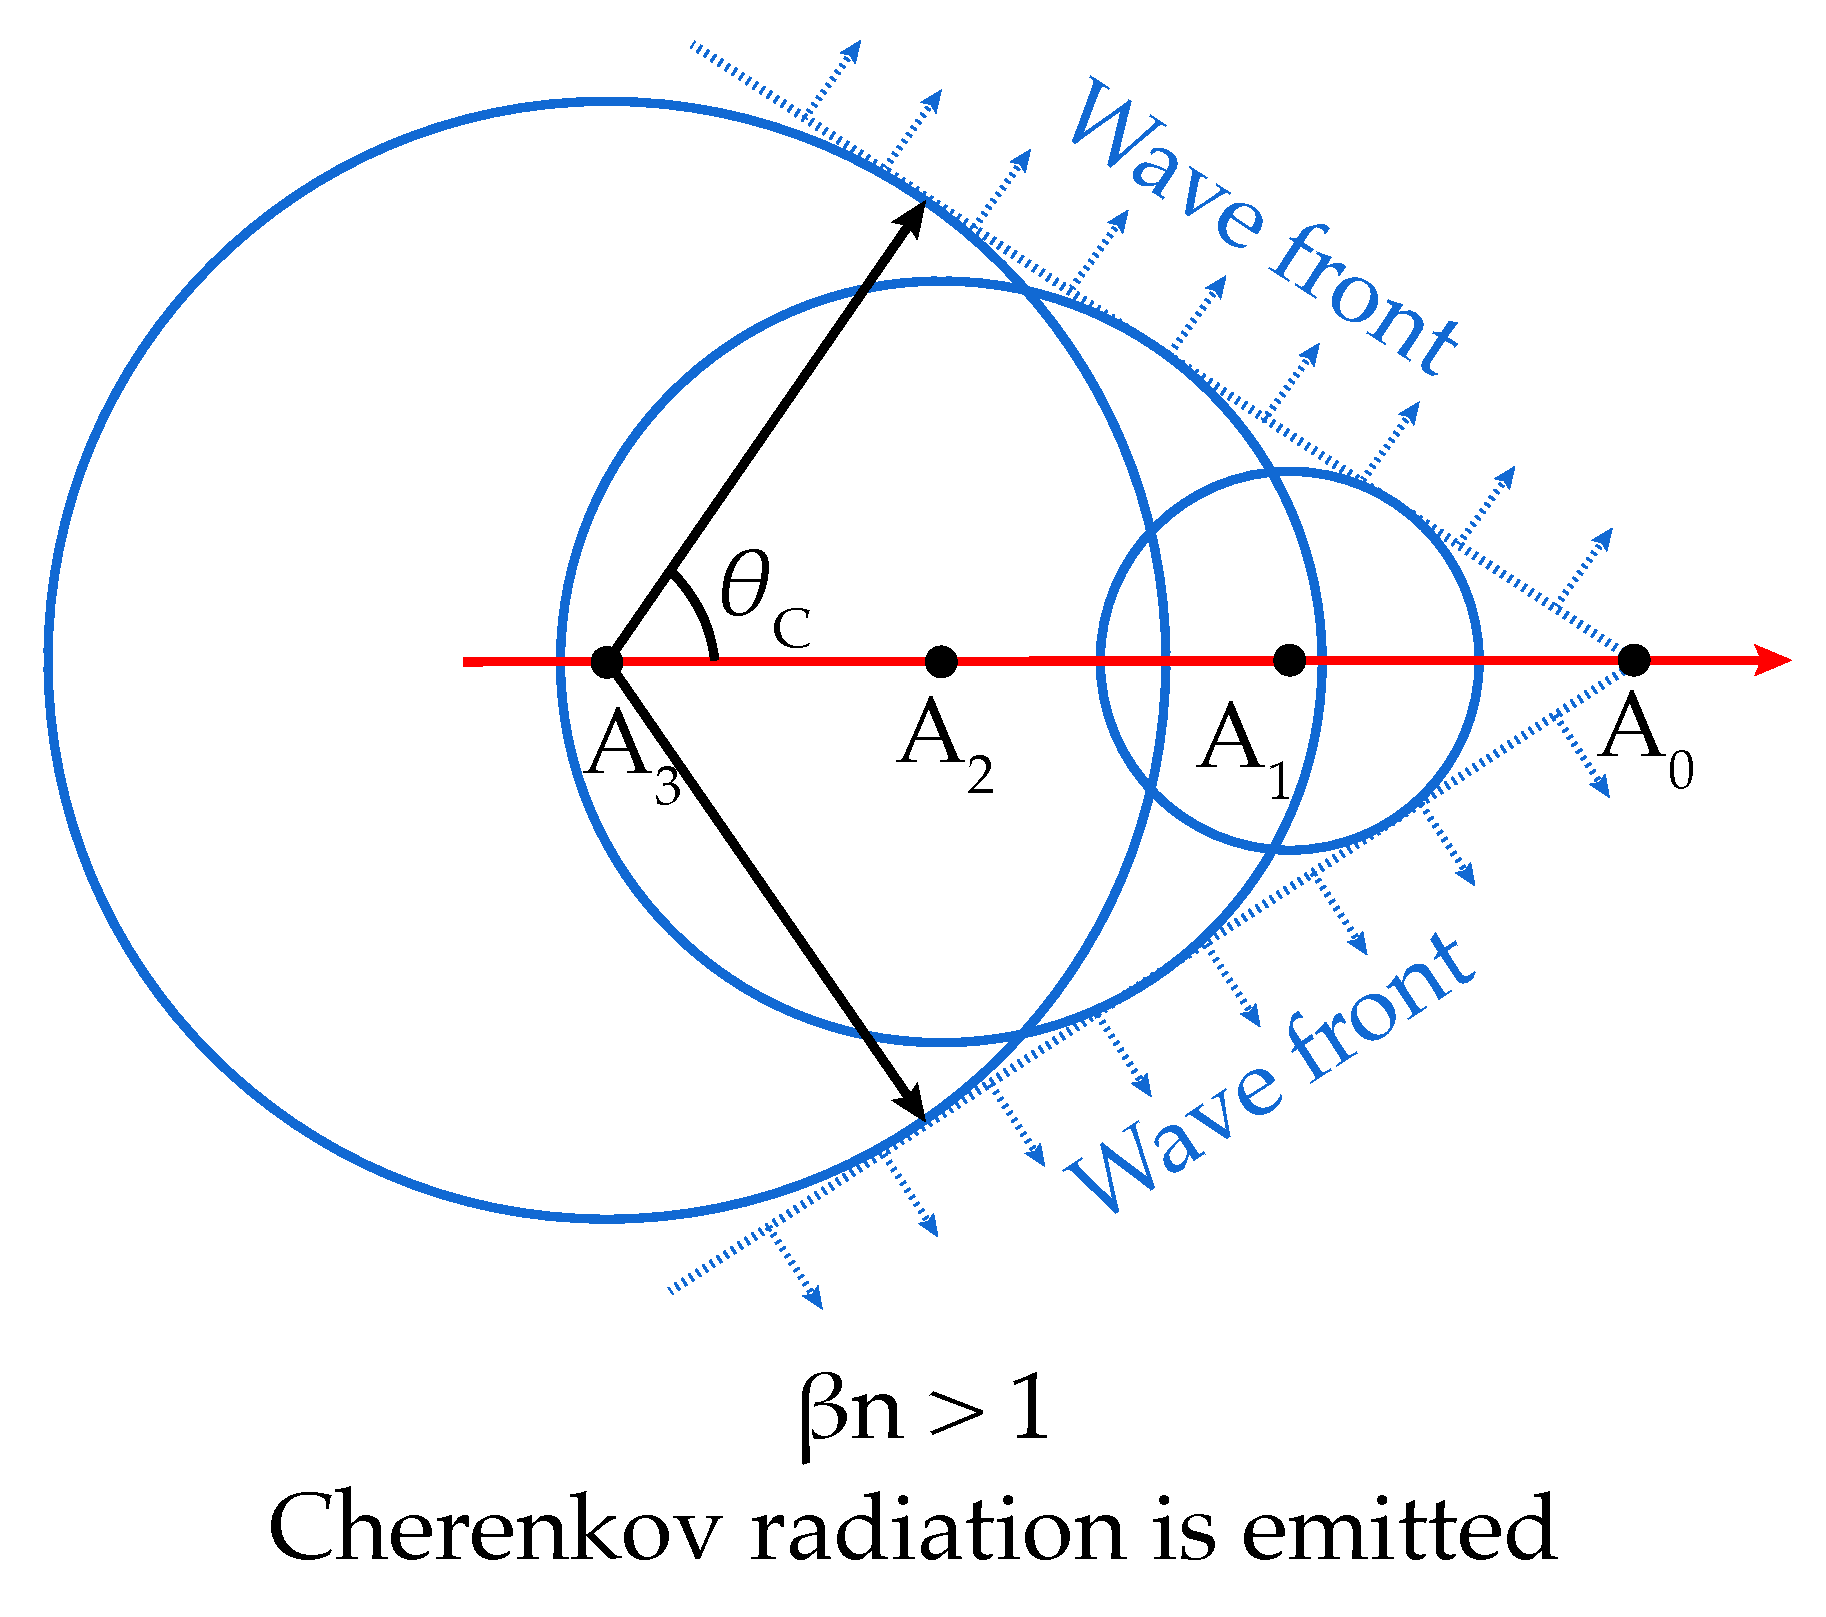
\includegraphics{ic/ic_cherenkov1.pdf}
    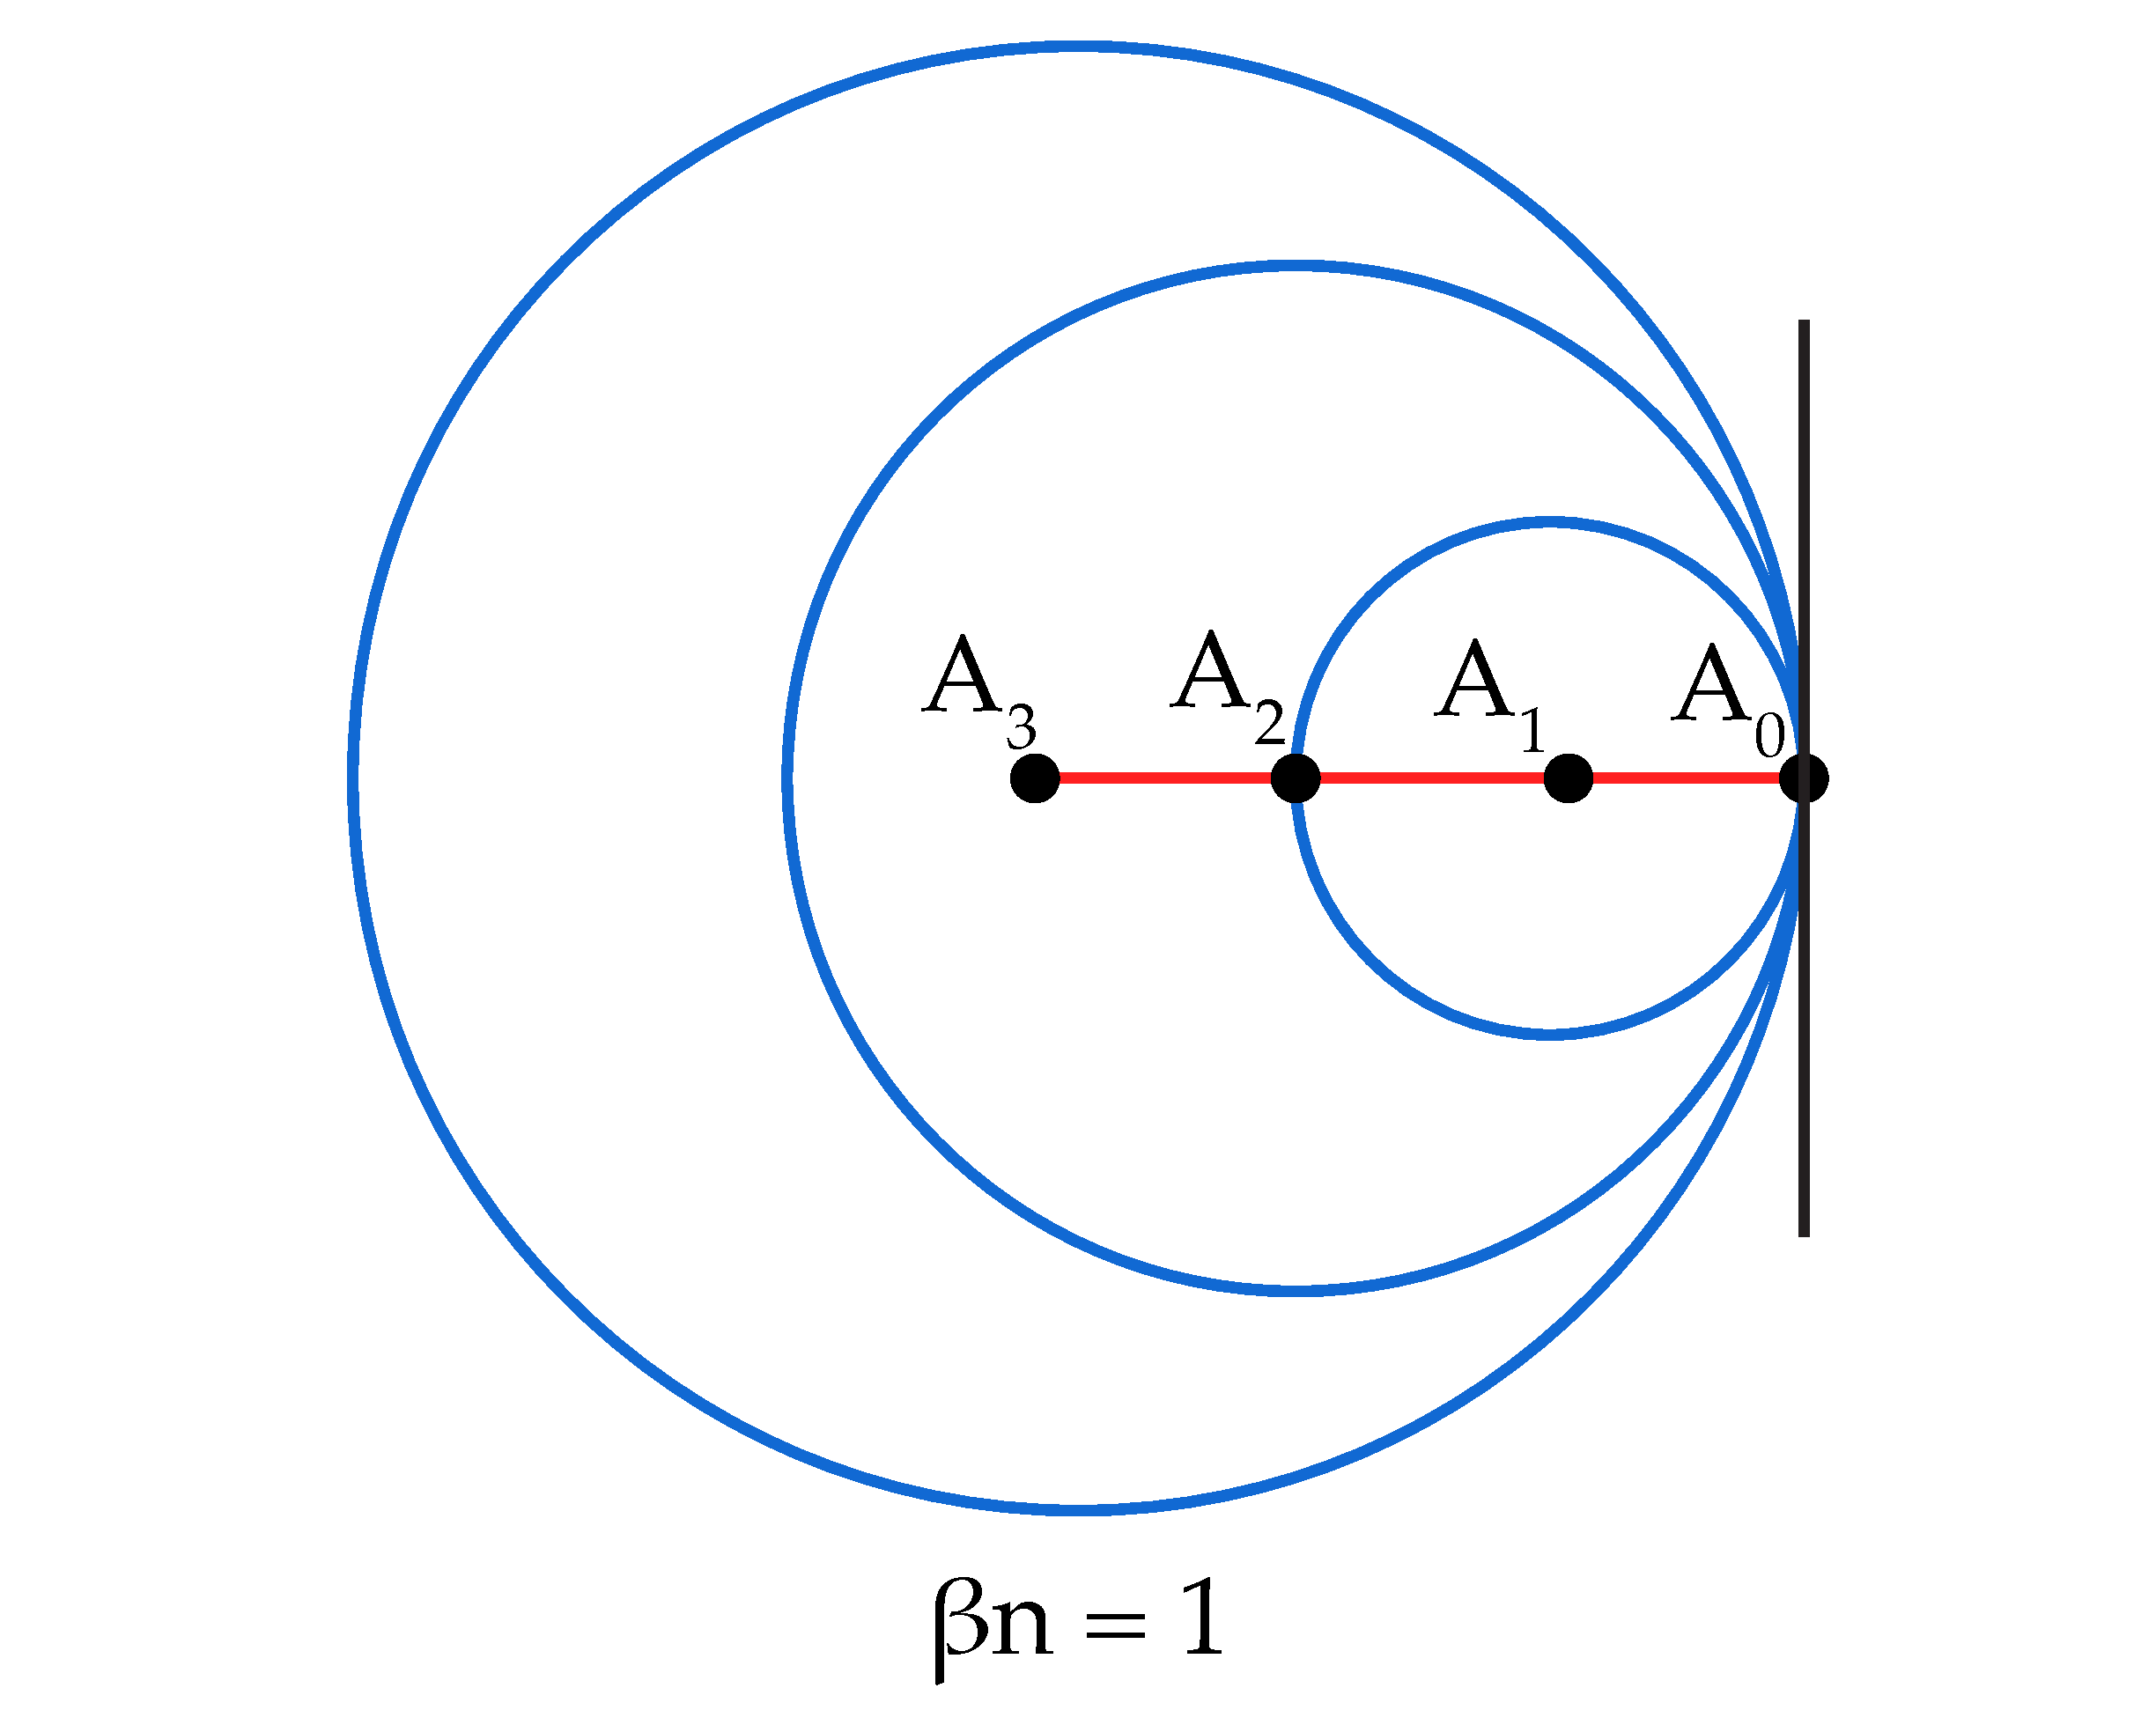
\includegraphics{ic/ic_cherenkov2.pdf}
    \caption[Cherenkov radiation]{The principle of Cherenkov radiation. In the upper figure Cherenkov radiation is emitted at the Cherenkov angle $\theta_\text{C}$, as the radiation emitted at different points in time forms a mutual, cone-shaped wavefront. In the figure on the bottom, all radiation is cancelled out by destructive interference (all circles are subsets of the first on the left, as the particle is not moving faster than light in the medium). Adapted from~\cite{LAnnunziata2020}.}
    \labfig{cherenkov}
\end{marginfigure}
The basic operational principle of IceCube (and already of AMANDA) is the detection of Cherenkov light within the Antarctic ice. When charged secondary particles created by neutrino interactions travel through the ice with an energy high enough, their speed can exceed the phase velocity of light in ice and they emit Cherenkov radiation. The detector consists of 5160 individual Digital Optical Modules (DOMs), buried deep in the ice and sensitive to the Cherenkov radiation.

\section{Cherenkov Radiation}\label{cherenkov_radiation}

Cherenkov radiation was first detected in 1934 by Soviet scientist Pavel Cherenkov~\sidecite{Cherenkov1934}. It occurs when charged particles travel within a medium with a velocity exceeding the speed of light in that very medium. The refractive index in a medium is defined as $n=\frac{c_0}{c_m}$, where $c_0$ is the speed of light in vacuum and $c_m$ is the phase velocity of light in that medium. Note that the phase velocity of light in a medium can exceed $c_0$, so $n<1$ is possible.

When charged particles cross an electrically neutral dielectric medium, atoms along the particle's path are briefly polarized. When they relax back to the ground state, the atoms emit electromagnetic radiation.

For non-relativistic particles, this radiation destructively interferes with itself, canceling out all signals (see the bottom panel of Fig.~\ref{fig:cherenkov}). But if the particle is traveling faster than the speed of light within the medium $c_m$, this destructive interference does not happen. Rather, a cone-shaped wavefront gets created (see top panel of Fig.~\ref{fig:cherenkov}). This wavefront constitutes Cherenkov radiation. If the particle has speed $v=\beta c_0$, the angle $\theta$ between the particle trajectory and the direction of the Cherenkov radiation can be calculated as~\sidecite{LAnnunziata2020}

\begin{equation}
    \cos{\theta} = \frac{\beta}{n}.
\end{equation}

If the medium is ice, to first order the refractive index $n$ is $\approx1.31$.\sidenote{This is of course rather crude. The $n$ of Antarctic glacial ice depends e.g.\ on depth; a fact we will come back to later when discussing directional reconstruction of high-energy IceCube neutrinos.} A secondary muon traveling through the ice at $0.999\,c_0$ will therefore emit Cherenkov light at an angle of $\theta = \cos^{-1}{\big(\frac{0.999}{1.31}\big)} \approx \SI{40}{\degree}$.
\begin{marginfigure}
    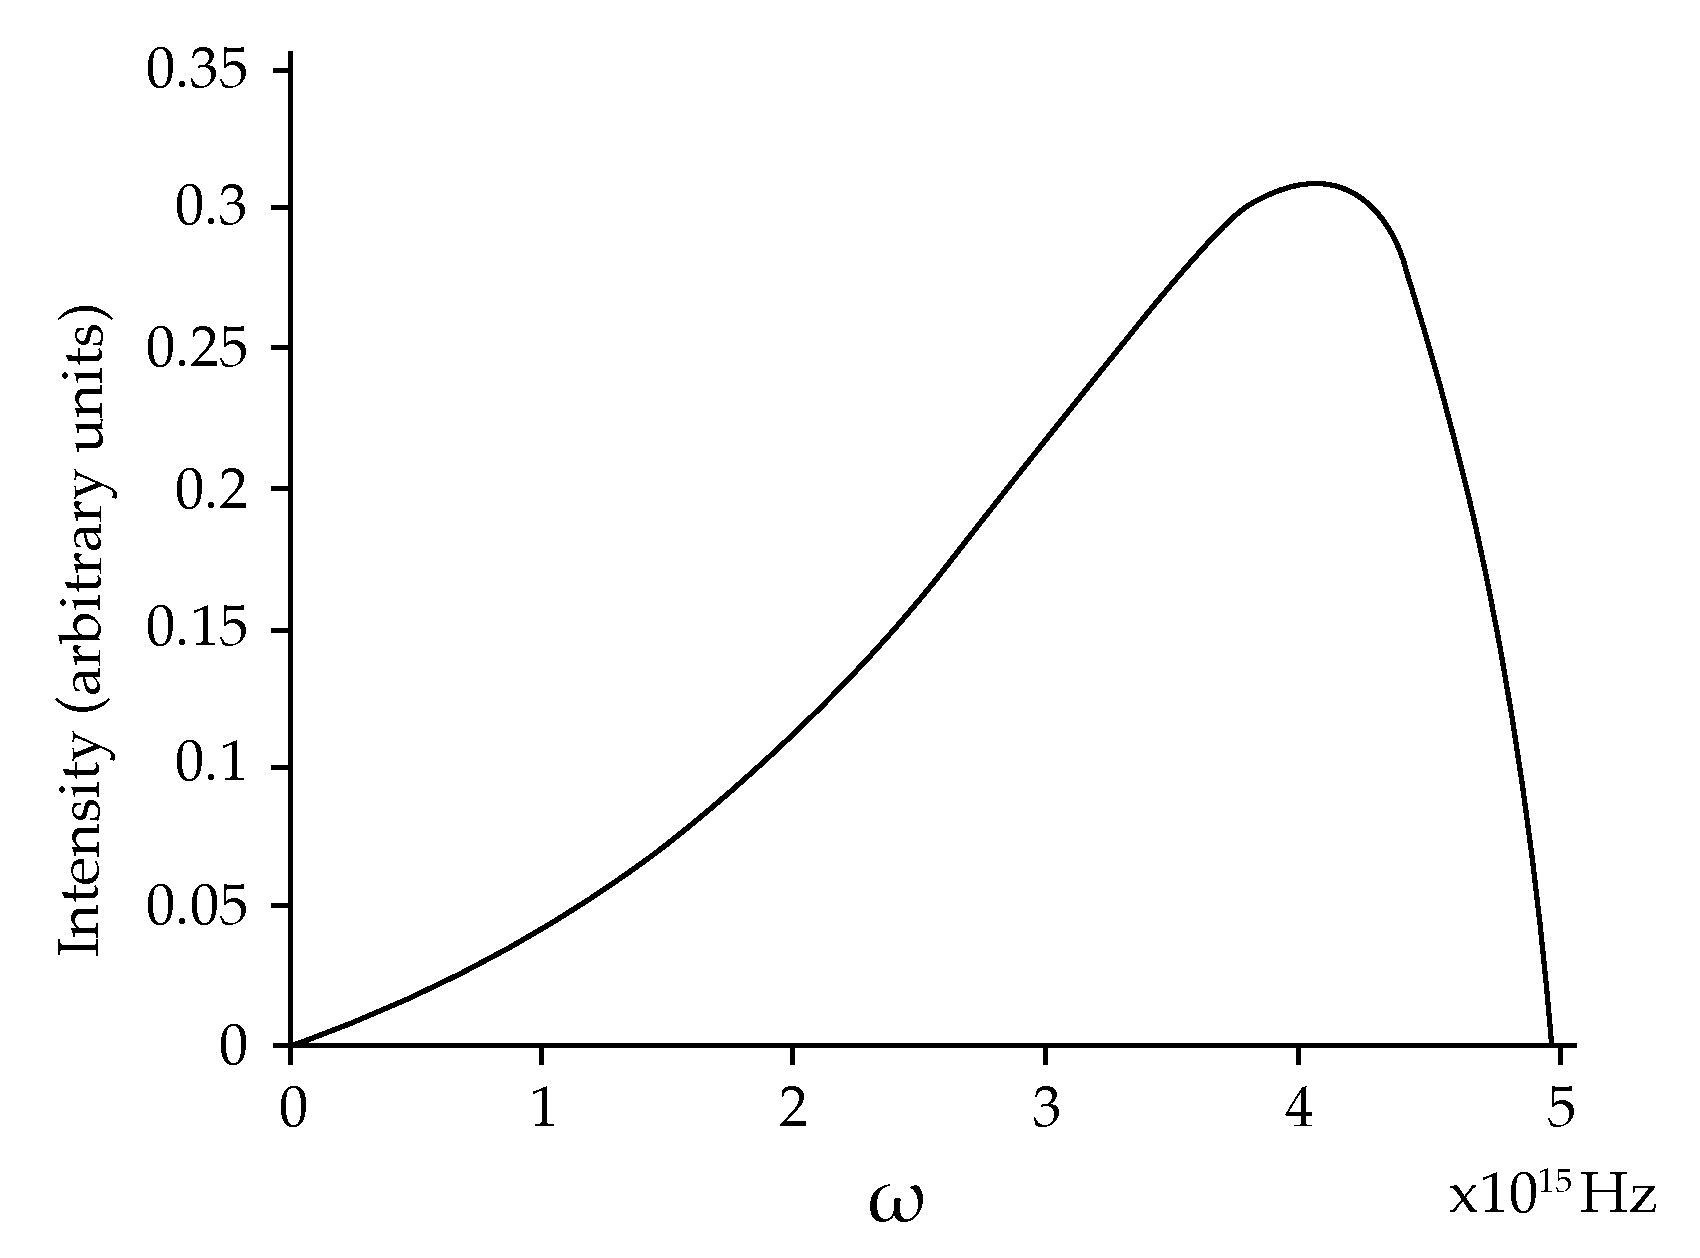
\includegraphics{ic/ic_cherenkov_spectrum.pdf}
    \caption[Cherenkov spectrum]{Cherenkov spectrum for a particle with $v=0.8 \,c_0$ in water. The intensity peaks at $\SI{4e15}{\Hz}$, corresponding to a wavelength of \SI{75}{\nm}, lying at the high-frequency end of the UV spectrum. Adapted from~\cite{Fulop1992}.}
    \labfig{cherenkov_spectrum}
\end{marginfigure}
Cherenkov radiation has a smooth spectrum, with a relative intensity roughly proportional to the frequency. Note that the refractive index of a medium also depends on the frequency, dropping below 1 in the X-ray. From this it follows that Cherenkov radiation appears blue to the human eye (the high-frequency part dominates) and its intensity peaks in the Ultra Violet (UV), before it sharply drops off in the X-ray regime~\sidecite{Fulop1992}, see Fig.~\ref{fig:cherenkov_spectrum}.

\section{Instrumentation}

IceCube detects neutrinos by observing the optical and UV part of their secondary particle Cherenkov spectrum (see Section~\ref{cherenkov_radiation} above). To understand how this is done, one first needs to look at the working principe of a Photomultiplier Tube (PMT), the basic instrument within the DOMs.

\subsection{Photomultiplier Tubes}
A PMT is a device used to detect very faint light signals by amplifying them. They consist of vacuum tubes and were successfully realized for the first time in the 1930s~\sidecite{Iams1935}.

\begin{figure}[h!]
    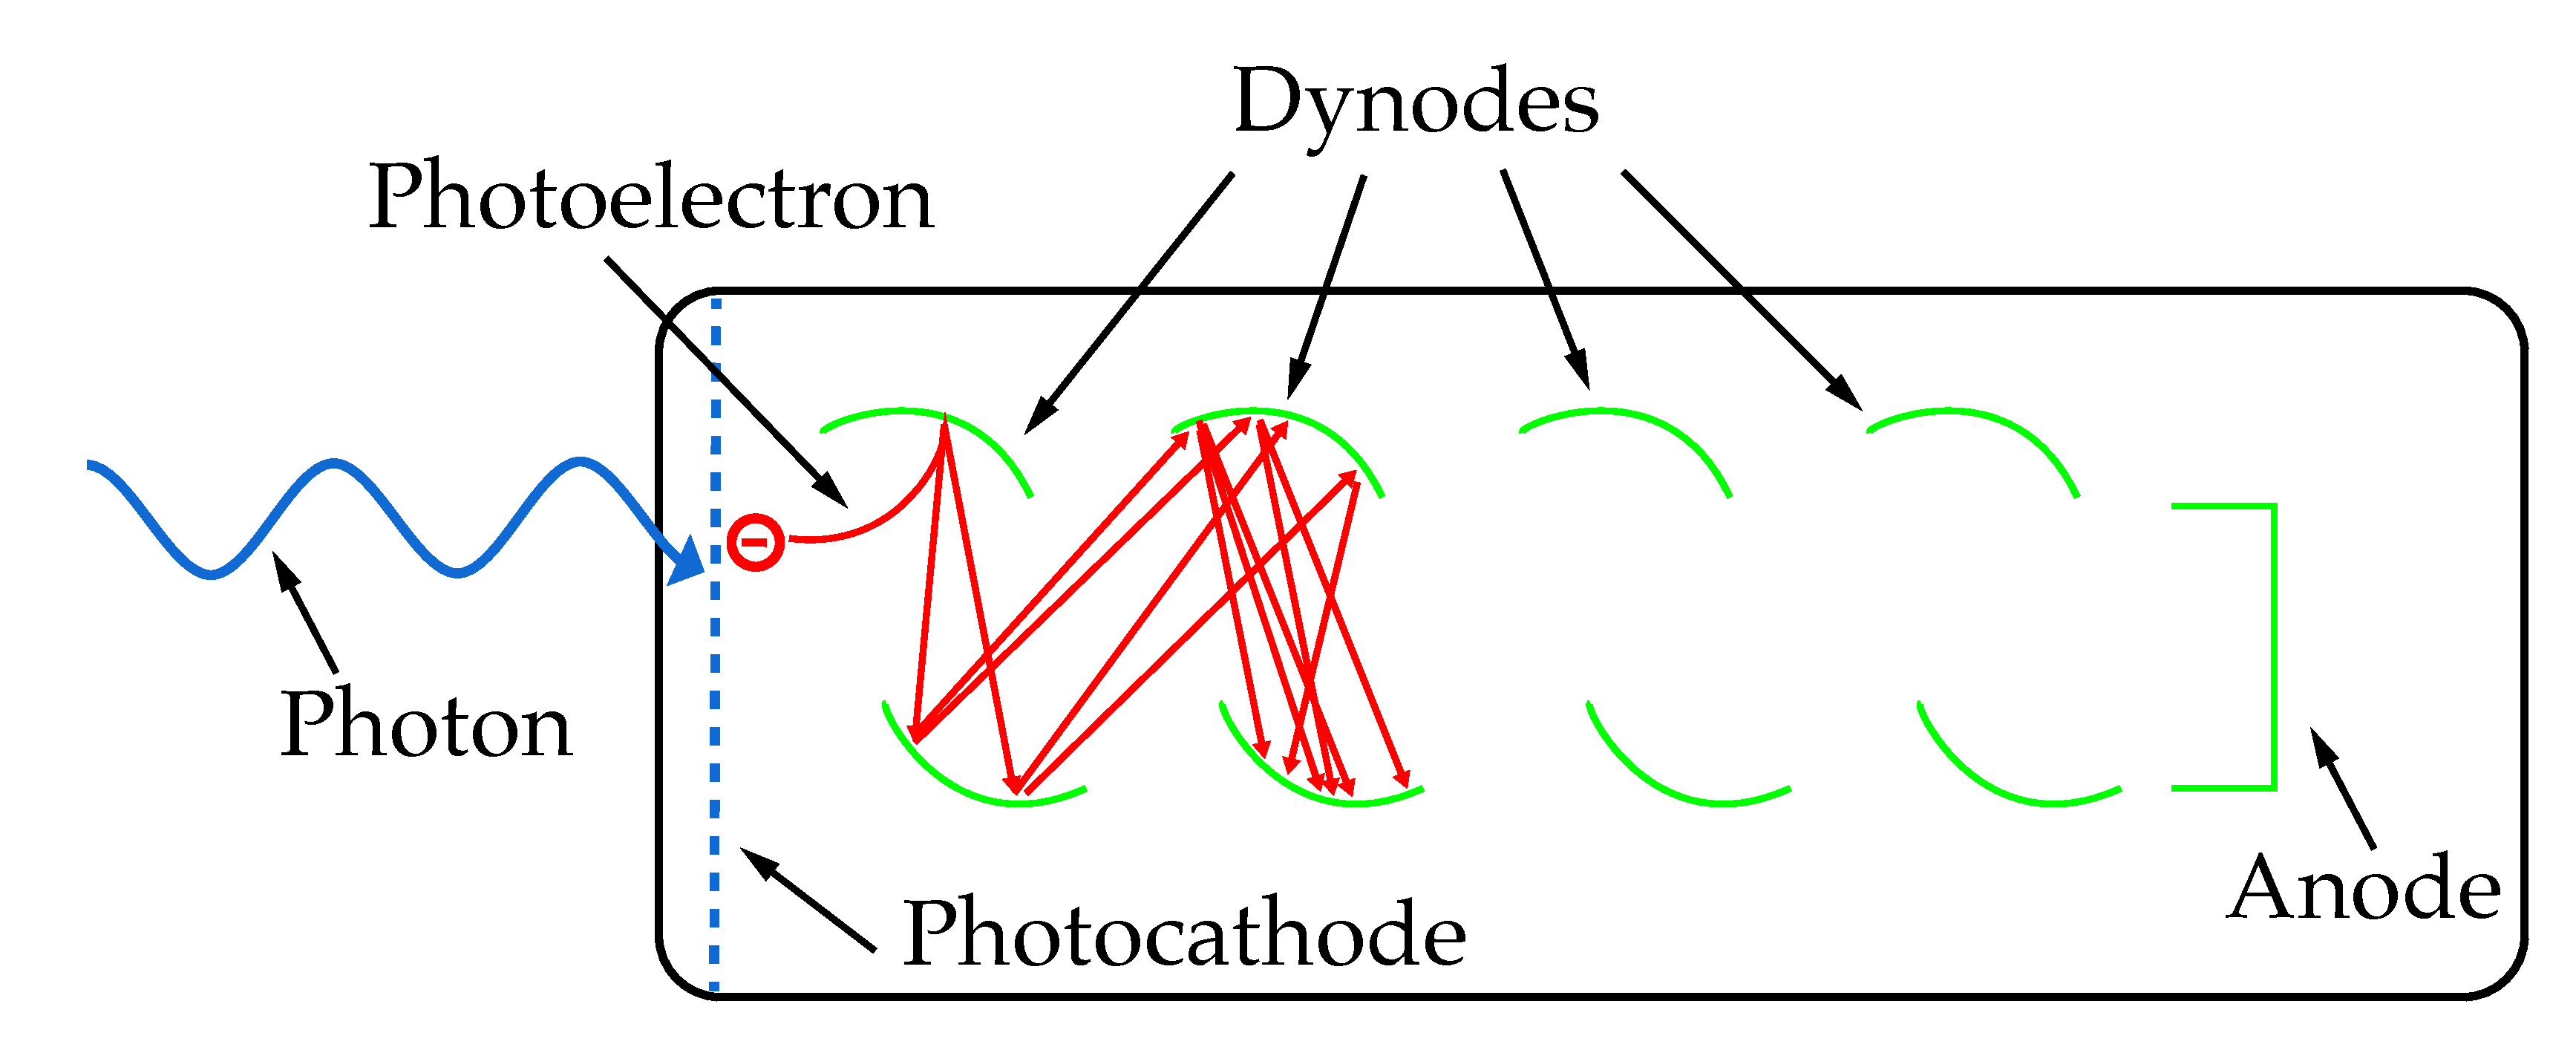
\includegraphics{ic/ic_pmt_annotated.pdf}
    \caption[PMT schematic]{A photomultiplier tube. Adapted from~\cite{Bednarski2014}.}
    \labfig{pmt}
\end{figure}

As one can see in Fig.~\ref{fig:pmt}, there are three principal components: a \textit{cathode}, several dynodes and an \textit{anode}. When photons hit the cathode, they can release electrons via the photoelectric effect~\sidecite{Einstein1905}. These photoelectrons are then accelerated (towards the right side in Fig.~\ref{fig:pmt}) by an electric field within the tube. This field is generated by applying a high voltage between the cathode and the anode.

To amplify the signal, a number of dynodes are placed between cathode and anode. These are additional electrodes with subsequently higher voltages. When the photoelectron hits the first dynode, a number of secondary electrons are generated, which are then accelerated towards the next dynode by the electric field. This process repeats for every dynode, generating an electron avalanche exponentially amplifying the original single photoelectron signal. The number of secondary electrons hitting the anode is proportional to the number of incident photons, resulting in a linear detector response (as long as the detector stays below its saturation limit)~\sidecite{Wright2017}.

IceCube uses PMTs made by Hamamatsu Photonics (R7081--02), sensitive to photons between 300 and \SI{650}{\nm}. They have a quantum efficiency (QE) at \SI{390}{\nm} of \SI{25}{\percent}, are operated with a voltage of \SI{1500}{\V} and have a gain (electron multiplication factor) of \num{e7}. The photon-sensitive surface area is typically \SI{530}{\cm\squared}~\sidecite{Abbasi2010}.

\subsection{The Digital Optical Module}\label{DOM}
\begin{marginfigure}
    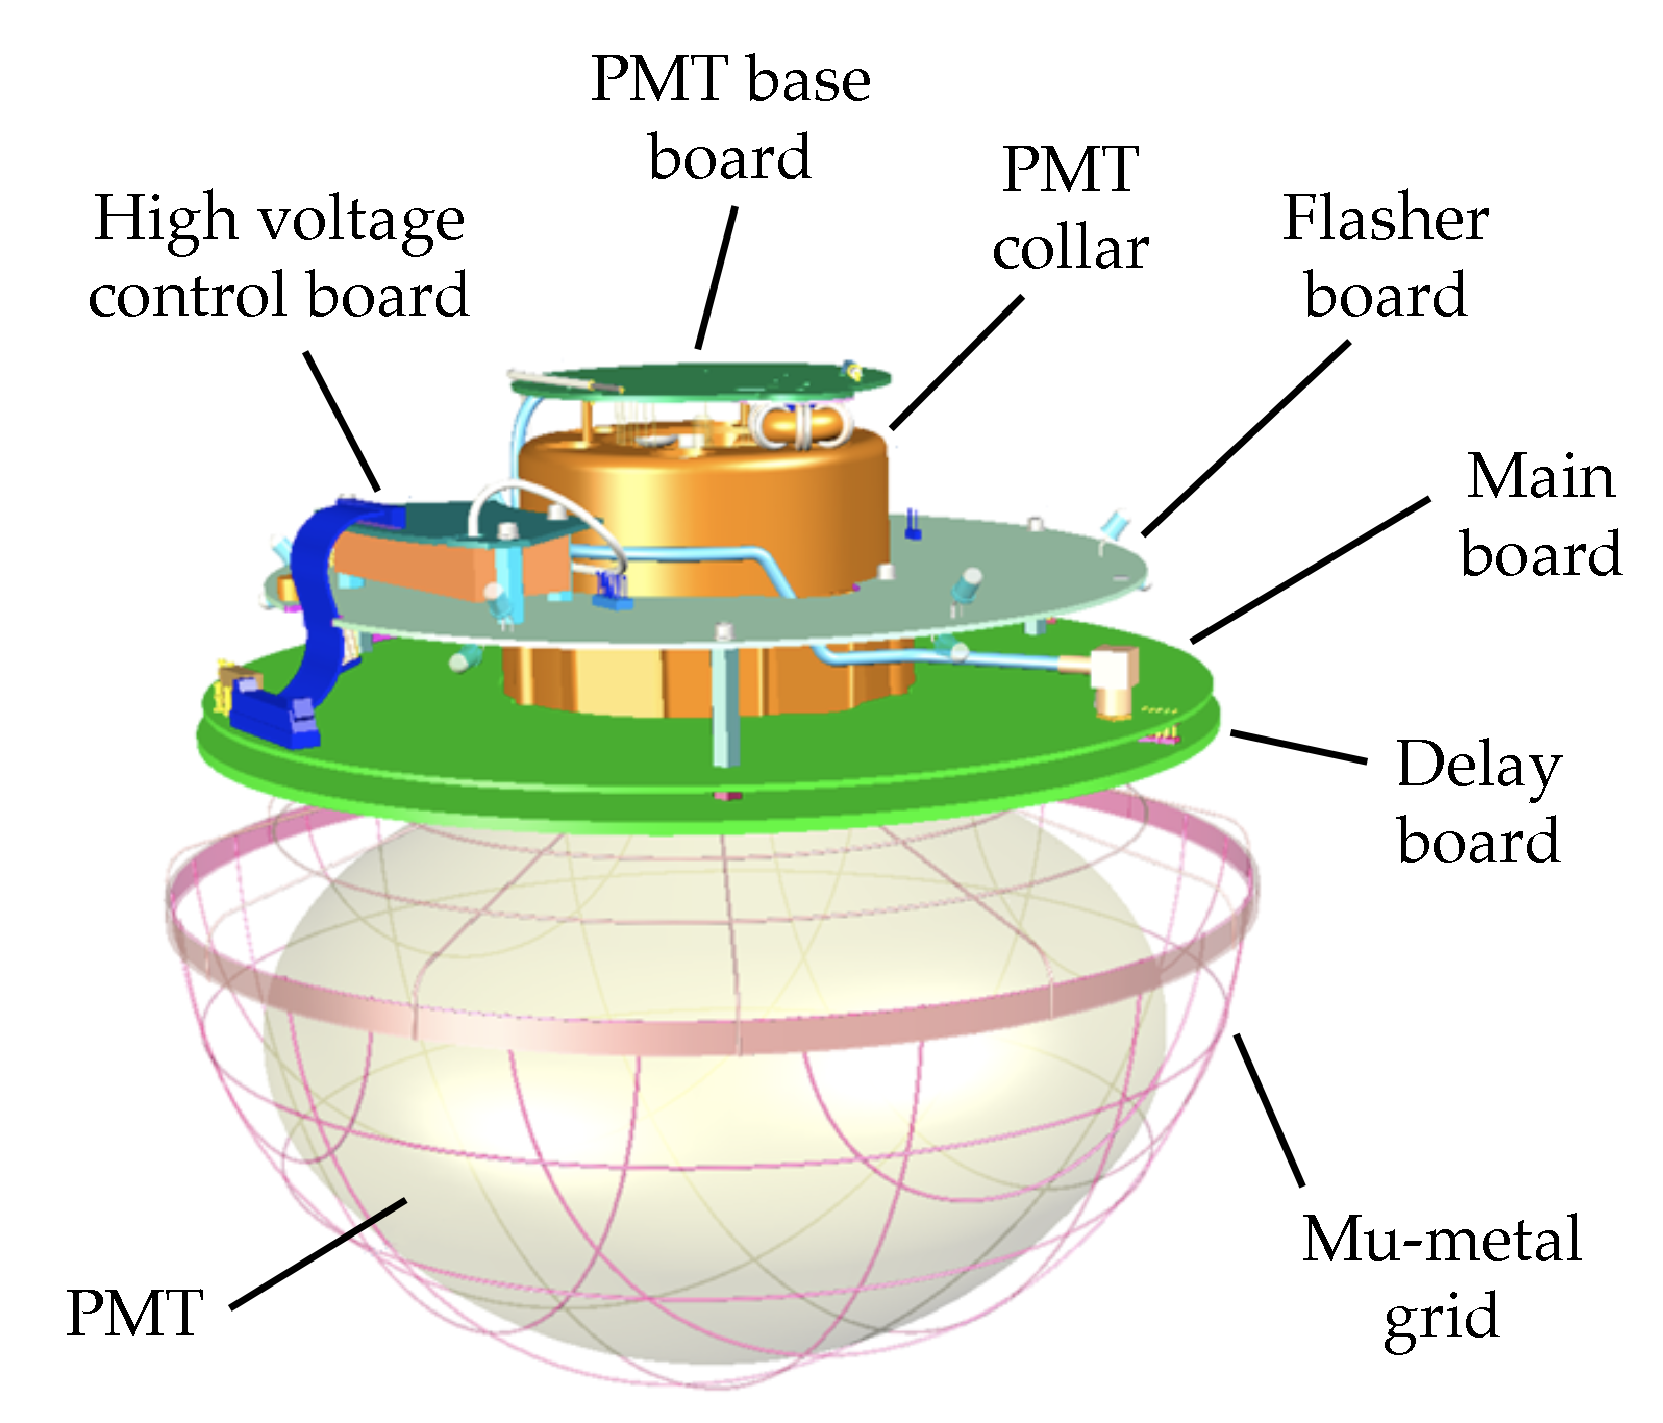
\includegraphics{ic/ic_DOM.pdf}
    \caption[IceCube digital optical module]{The IceCube DOM seen from the side. The detecting side of the PMT is facing downwards, with the main board and the PMT base board on top. From~\cite{Aartsen2017}.}
    \labfig{ic_dom}
\end{marginfigure}

The individual IceCube PMTs for detecting the Cherenkov radiation are enclosed in the DOMs. Each DOM consists of a pressure-resistant glass sphere, several controller boards and the PMT, facing downward (see Fig.~\ref{fig:ic_dom}). The glass sphere can withstand long-term pressure of \SI{250}{\bar}. The optical transmission of the spheres was measured to be \SI{93}{\percent} at \SI{400}{\nm}, decreasing to \SI{10}{\percent} at \SI{315}{\nm}.

The circular main board hosts data acquisition and control systems, as well as units for communication and a power converter. Another board interfaces with the PMT, while additional boards delay the PMT signals and generate the high voltage current powering the PMT. Additionally, there is a so-called \textit{Flasher Board} that controls Light-Emitting Diodes (LEDs). These are used to generate light flashes which can be received by neighboring DOMs for calibration purposes~\sidecite{Aartsen2017}.

\begin{marginfigure}
    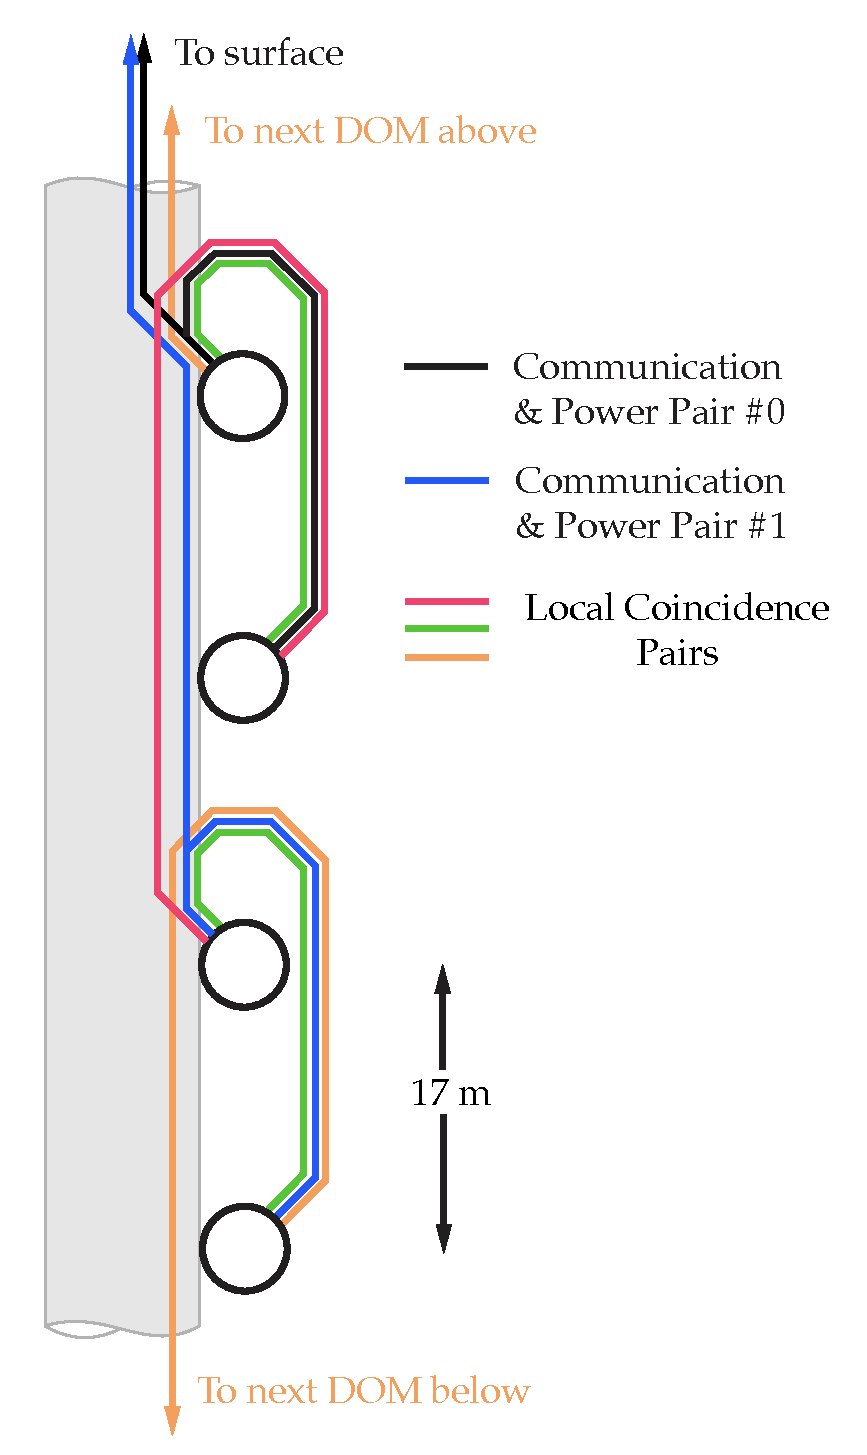
\includegraphics{ic/ic_DOM_connections.pdf}
    \caption[IceCube DOM connections]{Connection scheme for four IceCube DOMs along one string. Pairs of DOMs share one twisted-pair cable. Also, each DOM is directly connected to its direct neighbors above and below. Adapted from~\cite{Aartsen2017}.}
    \labfig{ic_dom_connections}
\end{marginfigure}

Because of data storage restrictions, the DOMs only record and digitize the photon signal after several trigger criteria have been met. The digitized voltage over time detected by the PMTs is called a waveform, and combined with a timestamp it comprises the basic datum in IceCube, a hit.

To fully record the waveform after a hit, the signal needs to be stored in a buffer. This is realized with the delay board, which routes the analog PMT signal through a \SI{10}{\m} long, serpentine copper trace to delay it by \SI{75}{\ns}.

When a hit is detected, the DOM sends a tag signal to the neighbor and next-to-nearest neighbor DOMs. When no neighbors detect a hit, the isolated hit only contains the timestamp, the amplitude and charge information extracted from the waveform. When at least two neighboring DOMs also detect a hit within \SI{0.25}{\micro\s}, a Local Coincidence (LC) is triggered. If the signal passes a threshold of 0.25 photoelectrons, the recorded waveforms are digitized and appended to the hits tagged as LC~\cite{Aartsen2017}.

The digitization of the PMT waveform is done with the Analog Transient Waveform Digitizer (ATWD), a custom-built Application Specific Integrated Circuit (ASIC). Usually lying dormant, the ATWDs start to capture the delayed waveform when the PMT discriminator initiates it. The captured waveforms are only digitized in case a hit (i.e.\ local coincidence) is registered~\cite{Aartsen2017}.

The DOMs are connected to the IceCube Laboratory (ICL) with twisted-pair copper cables. The power for the DOM is also transmitted with this cable. Two DOMs share one twisted-pair cable, and each DOM is also directly connected to its two neighbors on the same string. Fig.~\ref{fig:ic_dom_connections} shows the connection layout.

The Flasher Board houses 12 LEDs operating at \SI{\sim400}{\nm} wavelength. These are used to verify the DOM timing response, to measure the DOM in-ice position, to determine the optical properties of the ice, and to verify the reconstruction algorithms~\cite{Aartsen2017}.

\subsection{Detector Layout}
In total, approximately 5800 DOM units were built and tested, 300 failing tests and the rest being delivered to the South Pole. The vast majority of these were ultimately deployed (5160 in total). The final detector layout (since the last drilling campaign 2010/2011, see below) consists of 86 strings. The DOMs were deployed along those strings, like pearls on a necklace. Each string contains 60 DOMs, with an average horizontal spacing between strings of \SI{125}{\meter}~\cite{Aartsen2017}.

\begin{figure}
    \includegraphics[width=1.\textwidth]{ic/ic_side_view_font.pdf}
    \caption[IceCube side-on]{Side view of the IceCube detector, showing the instrumented array deep in the Antarctic glacial ice. In the center on top is the IceCube Laboratory, were data processing takes place. From~\cite{Ahlers2018a}.}
    \labfig{ic_sideon}
\end{figure}
\begin{marginfigure}
    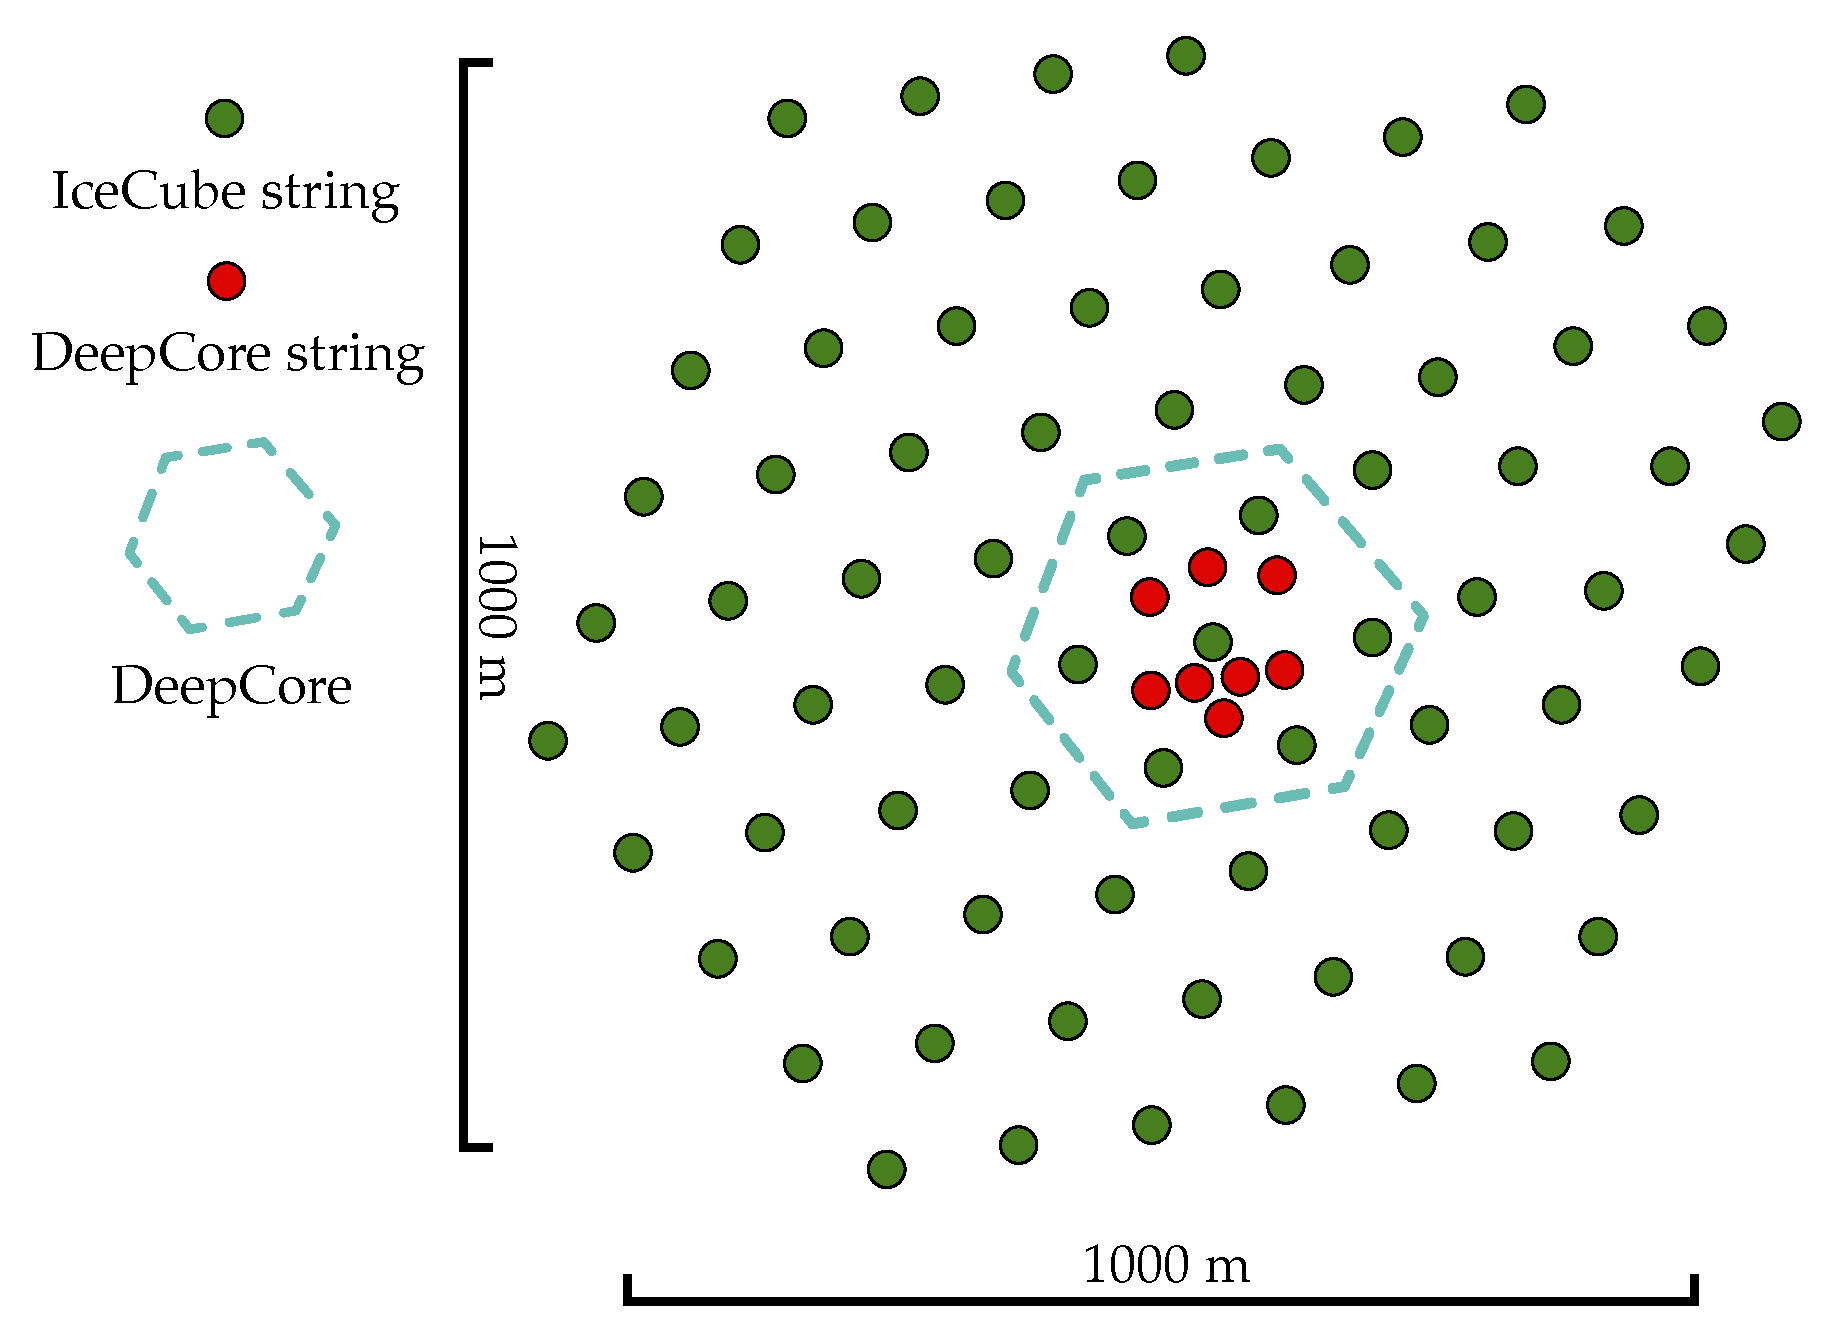
\includegraphics{ic/ic_top_view.pdf}
    \caption[IceCube top-down view]{Top-down view of the IceCube detector, spanning \SI{1}{\square\km} on the surface. From~\cite{Ahlers2018a}.}
    \labfig{ic_top_down}
\end{marginfigure}

The instrumented part of the strings starts at \SI{1450}{\m} below surface, with one DOM every \SI{17}{\m} to a depth of \SI{2450}{\m}, just above the bedrock at a depth of \SI{2820}{\m}. In Fig.~\ref{fig:ic_sideon} the layout of the in-ice array can be seen. The strings follow a roughly hexagonal layout (see Fig.~\ref{fig:ic_top_down}), with a side length of \SI{1}{\km\squared}. The total instrumented volume of glacial ice is thus \SI{1}{\km\cubed}~\cite{Aartsen2017}. Of the 5160 deployed DOMs, 92 are dead as of March 2023, a loss of \SI{1.7}{\percent}\sidenote{This is better than the predicted failure percentage, which was projected to be \SI{2}{\percent} by 2023~\cite{Aartsen2017}.}.

One can see in Fig.~\ref{fig:ic_top_down} that there is a region in the center of the detector which is more densely instrumented: The strings are closer to each other, and also the spacing between DOMs on these strings is reduced from \SI{17}{\m} to \SIrange{7}{10}{\m}. This part of the detector is DeepCore, designed to have a lower energy threshold of \SI{10}{\GeV}, a significant improvement over the \SI{100}{\GeV} for the rest of the detector. The DOMs within DeepCore are also modified for this goal, as they are equipped with PMTs that have a \SI{35}{\percent} higher QE compared to the `normal' DOMs~\cite{Aartsen2017}.


\subsection{Deployment}
As one can imagine, embedding the DOMs within the ice was a non-trivial task. It required drilling 86 boreholes with a diameter\sidenote{The hole diameter was larger than the DOM diameter (\SI{35}{\cm}) to account for partial refreezing of the bore hole.} of roughly \SI{60}{\cm} and a length of \SI{2500}{\m}. This was achieved over several drilling campaigns with the Enhanced Hot Water Drill (EHWD) specifically built for this task. This drill had a total power of \SI{5}{\mega\W} and was able to drill with a maximum speed of \SI{2.2}{\meter\per\minute}. With these performance characteristics, one hole was drilled every \SI{48}{\hour} on average\sidenote{Drill operation happened around the clock.}~\cite{Aartsen2017}. It took 7 drilling seasons to deploy the final IceCube86 setup, from the Antarctic summers 2004/2005 to 2010/2011. Fig.~\ref{fig:ic_drill} shows the tower operations site directly above the bore hole~\sidecite{Benson2014}.

The water for drilling the holes was heated to \SI{88}{\celsius} with 35 water heaters working in parallel, each providing \SI{125}{\kilo\W} power. The average amount of fuel used per drill hole was \SI{27000}{\liter}~\cite{Benson2014}.

\begin{figure}[]
    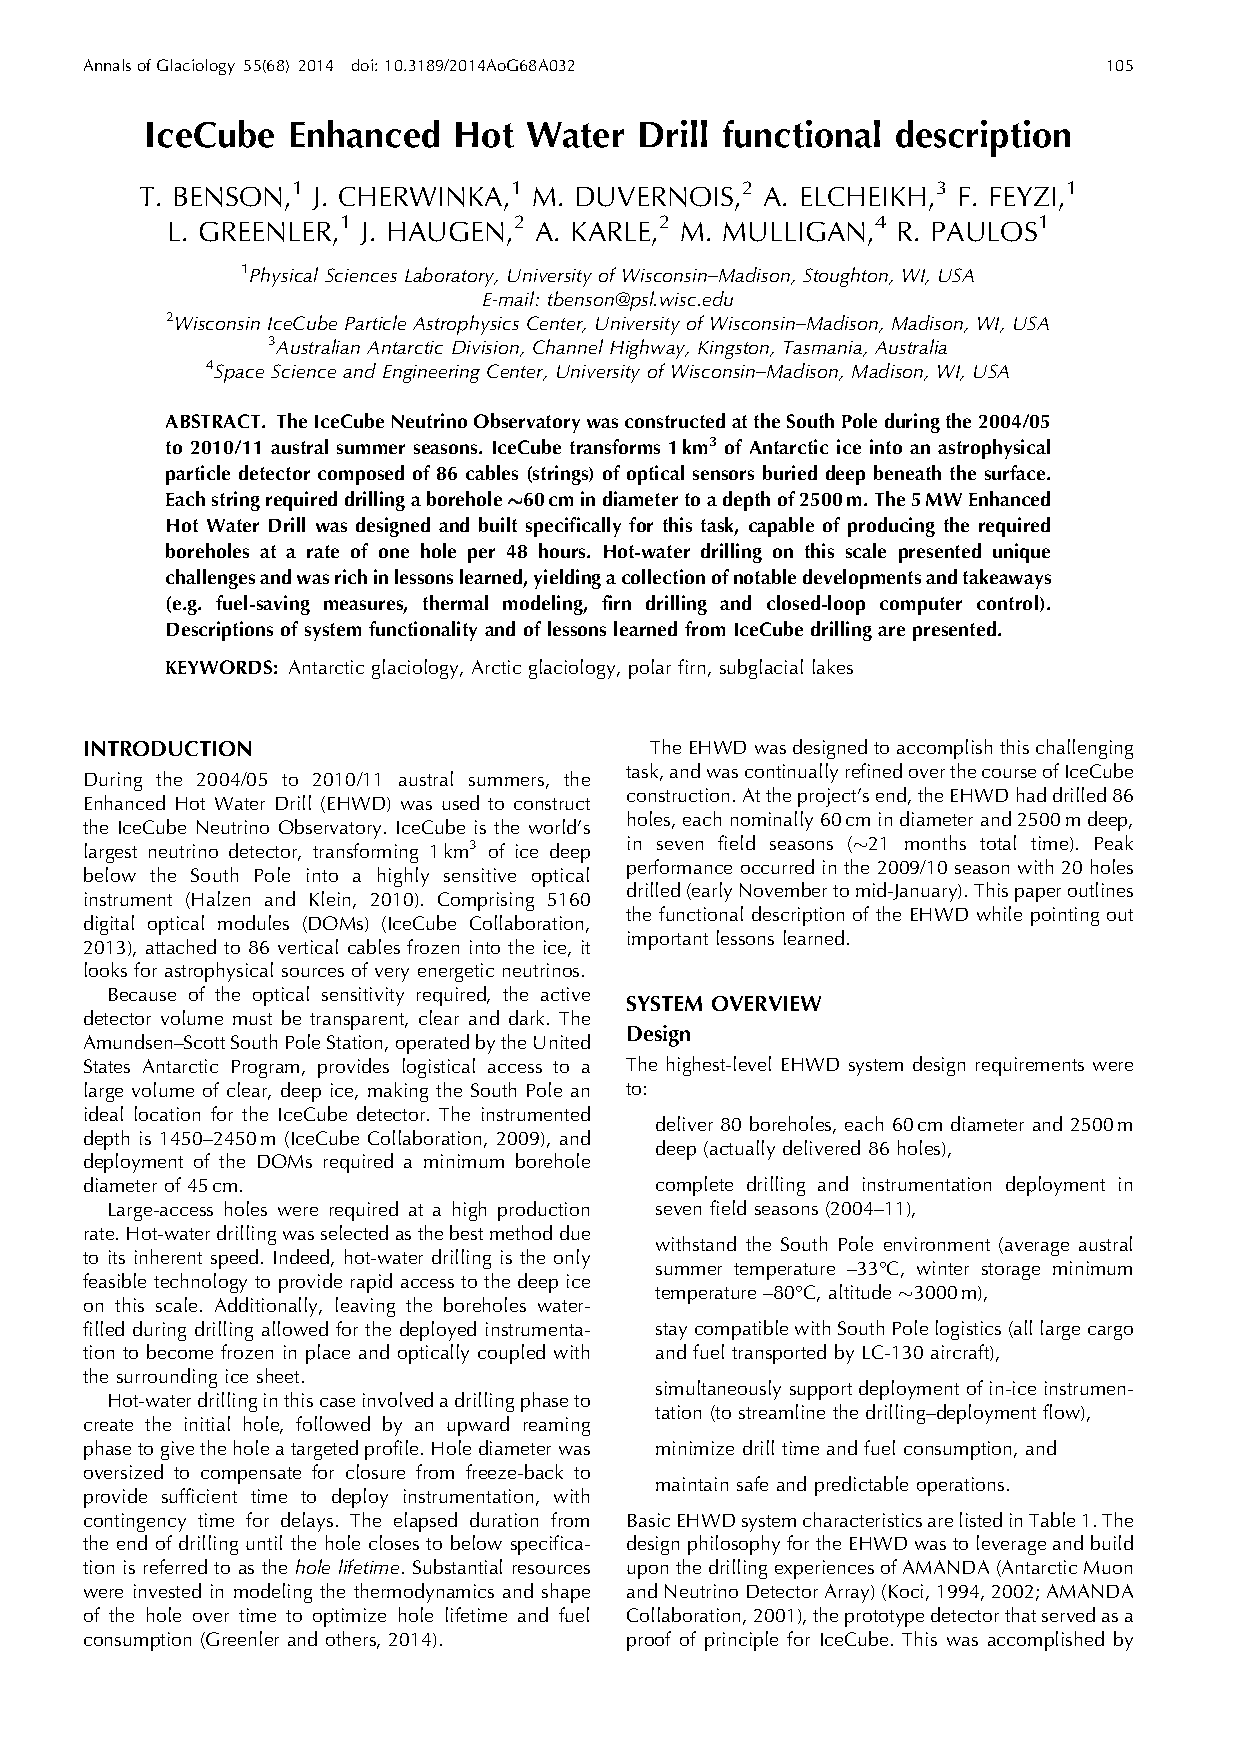
\includegraphics{ic/ic_drill.pdf}
    \caption[IceCube enhanced hot water drill]{The hole drilling part of the IceCube Enhanded Hot Water Drill, excluding the hot, pressurized water supply. One can see the tower operations site (TOS) above the hole and the hoses providing hot water and returning cooled water from the bore hole to the generators in a closed loop. From~\cite{Benson2014}.}
    \labfig{ic_drill}
\end{figure}

\subsection{The IceTop Surface Array}

\begin{marginfigure}
    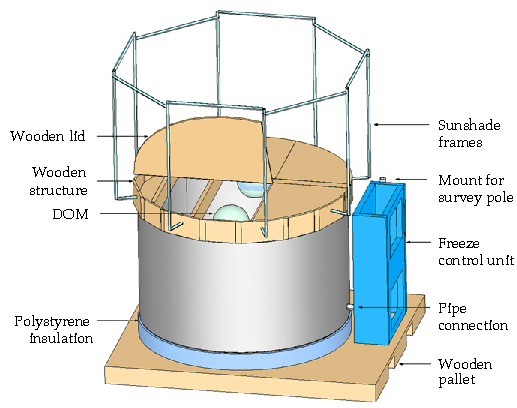
\includegraphics{ic/ic_icetop.pdf}
    \caption[IceTop detector]{IceTop surface Cherenkov detector tank. From~\cite{Abbasi2013}.}
    \labfig{ic_icetop}
\end{marginfigure}

In addition to the in-ice detector, IceCube has a surface air shower detector for cosmic-ray physics\sidenote{See Section~\ref{cosmic_rays}.}, named IceTop. It was designed to study the cosmic-ray mass composition by correlating the energy it measures on the surface with the energy deposited by muons in the ice as measured by the in-ice detector~\sidecite{Abbasi2013}. The energy sensitivity range of IceTop is \SI{300}{\tera\eV} to \SI{1}{\exa\eV}~\sidecite{Aartsen2013a}.

The IceTop surface array consists of $2\times81$ ice-filled Cherenkov tanks. These are placed in pairs on the same hexagonal grid as the DOM strings for the in-ice array. Each tank is equipped with two standard IceCube DOMs (see Section~\ref{DOM})~\cite{Abbasi2013} which are operated at two different gain levels to increase the dynamic range.

Results from 3 years of IceTop data show good agreement between models describing the transition from galactic to extragalactic cosmic rays at energies above the knee. In these, the spectrum of lighter elements softens earlier towards higher energies compared to heavier elements. This is indeed reflected in the data~\sidecite{Aartsen2019}.

Furthermore, IceTop can be used to increase the purity of a sample of astrophysical neutrinos by using it to veto muon events that mostly stem from cosmic-ray induced air showers, as opposed to muons created by neutrino interactions~\sidecite{Amin2021} (more details on background rejection will follow in Section~\ref{background}).

\subsection{Data Acquisition}\label{data_acquisition}
As noted above, only for locally coincident hits in multiple detectors the full waveforms are digitized by the DOMs. These are then sent to the IceCube Laboratory on the surface via the twisted-pair cable datalink, were all DOM data is ingested into the data acquisition system (DAQ). Hits throughout the detector are investigated by the system to establish common causility by temporal and sometimes spatial patterns. All hits for which common causality can be established form an event. The rate of these events varies seasonally with the atmospheric muon flux, with a median event rate of \SI{2.7}{\kilo\Hz} and a total data rate of \SI{1}{\tera\byte\per\day} (roughly \SI{100}{\mega\bit\per\second})~\cite{Aartsen2017}.

Satellite bandwidth is limited and costly. Therefore, further on-site software triggers reduce the data rate to \SI{15}{\percent} of the initial rate. These events are then transmitted via satellite to the IceCube data center at the University of Wisconsin-Madison for further analysis. The full event stream is also written to redundant disks, which are transferred twice per year to Madison.

\subsection{Time Synchronization}
Precise timing information is crucial to reconstruct an event (see Section~\ref{reconstruction}). For this reason, all DOMs need to be synced to a common clock. This is achieved by syncing the whole system to a Symmetricom ET6000 GPS receiver. The synchronization of individual DOMs is performed once per second, while data transfer is paused during the process\sidenote{The calibration sequence takes $\lesssim$\SI{1.3}{\milli\second}}~\sidecite{Abbasi2009}.

IceCube ensures temporal synchronizity with an algorithm called Reciprocal Active Pulsing (\texttt{RAPcal}): A bipolar pulse is initiated on the surface and sent to the DOM. The sender saves the local time when it sends the pulse and starts a timer. Upon reception down the string, the DOM also saves its current local time, saves the received pulse waveform, starts a timer, responds with a bipolar pulse of its own and stops the timer. Upon reception, the surface station stops its timer and requests the received pulse waveform and all timing information from the DOM.

With these six pieces of information --- the two transmit timestamps, the two receive timestamps and both waveforms --- a transformation from the GPS-synchronized surface to local DOM time domain and vice versa can be calculated, with a precision of \SIrange{1}{2}{\ns}~\cite{Abbasi2009}.

\section{Angular Reconstruction}\label{reconstruction}

The goal of IceCube reconstruction is twofold: Reconstructing the deposited neutrino energy, and reconstructing the neutrino arrival direction. With this in mind, one can sort the events seen by the detector broadly into two categories: Well localized track events with poorly reconstructed energy, and cascade events with well-determined energy, but very imprecise origin.

\subsection{Event Types}\label{ic_event_types}

\begin{marginfigure}
    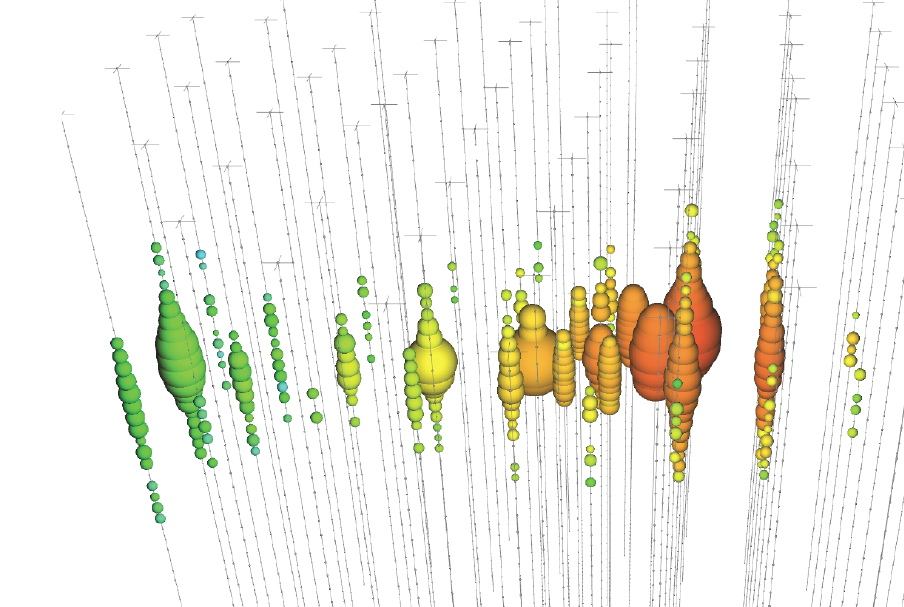
\includegraphics{ic/ic_track.png}
    \caption[Track event in IceCube]{Cascade event: The long track allows for good angular reconstruction, with high uncertainty on the event energy. From \url{masterclass.icecube.wisc.edu}.}
    \labfig{ic_track}
\end{marginfigure}
\begin{marginfigure}
    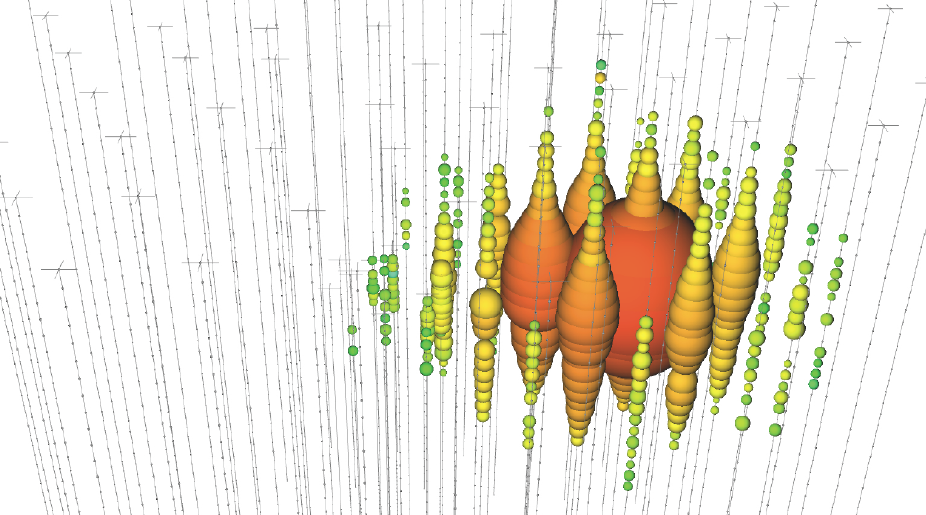
\includegraphics{ic/ic_cascade.png}
    \caption[Cascade event in IceCube]{Cascade event: The energy is fully contained in the detector, as the event is relatively isotropic. The angular uncertainty is quite large though. From \url{masterclass.icecube.wisc.edu}.}
    \labfig{ic_cascade}
\end{marginfigure}
\begin{description}
    \item[Track Events] (Fig.~\ref{fig:ic_track}) are produced by secondary muons resulting from the charged-current interaction of muon neutrinos with the Antarctic glacial ice (see section~\ref{neutrinos_current}). The secondary muons leave tracks in the ice with a length on the order of kilometers. Muons with energies above \SI{\sim300}{\giga\eV} create tracks that exceed the detector length. In general, this allows for a good angular resolution, ranging from \SI{1}{\degree} for a \SI{1}{\TeV} muon to \SI{0.3}{\degree} for a \SI{1}{\peta\eV} muon~\sidecite{Abbasi2022}. The drawback is a large energy uncertainty of $0.25 \log{E_\mu}$ for a muon of energy $E_\mu$~\sidecite{Aartsen2014a}, as parts of the high-energy muon tracks lie outside the instrumented volume~\sidecite{Aartsen2017a}.

    \item[Cascade Events] (Fig.~\ref{fig:ic_cascade}) on the other hand are initiated by the charged-current interactions of $\nu_e$ and $\nu_\tau$, as well as by neutral-current interactions from neutrinos of all flavors. They are usually relatively isotropic and contained within the detector, as typical track lengths are of $\mathcal{O}(\SI{10}{\meter})$. Their relative isotropicity only allows for poor angular resolution (\SIrange{10}{15}{\degree}), but comparably good energy reconstruction ($\frac{\delta E}{E} \approx \SI{15}{\percent}$)~\cite{Aartsen2017a}.
\end{description}

As this thesis is concerned with the sources of high-energy astrophysical neutrinos and the angular resolution of track events allows for a better pointing accuracy compared to cascade events, the next section will focus on the angular reconstruction of the former.

\subsection{Likelihood Approach}
The main angular reconstruction algorithm for muon tracks used in IceCube is based on the work done for AMANDA. It employs a maximum-likelihood method~\sidecite{Ahrens2004}. This can be understood as follows: Given a set set of unknown track parameters $\vec{a}$ and a set of experimentally determined values $\vec{x}$, what values of the unknown parameters $\vec{a}$ do maximize the probability of measuring the actually observed values $\vec{x}$?

This likelihood is denoted $\mathcal{L}(\vec{x}|\vec{a})$. If the components $x_i$ of $\vec{x}$ are independent, it can be expressed as

\begin{equation}
    \mathcal{L}(\vec{x}|\vec{a}) = \prod_i p(x_i|\vec{a}).
\end{equation}

Here, $p(x_i|\vec{a})$ is the probability density function (PDF) of measuring $x_i$ given a set of parameters $\vec{a}$. The reconstruction consists in obtaining the set of unknown track parameters $\vec{a}$ that maximizes the likelihood $\mathcal{L}$ (or, for technical reasons, minimizes $-\log{\mathcal{L}}$).

\subsection{Parametrization}
\begin{figure}[htb]
    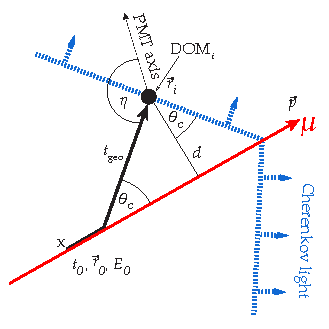
\includegraphics[width=0.6\textwidth]{ic/amanda_reco.pdf}
    \caption[Angular reconstruction in IceCube]{Parametrization for the angular muon reconstruction, describing the trajectory of a muon (red line) with energy $E_0$ that is in position $\vec{r_0}$ at time $t_0$, traveling towards direction $\vec{p}$. Cherenkov light from that muon is detected by a DOM at position $\vec{r_i}$ at distance $d$ to the trajectory with a light travel time $t_\text{geo}$. Adapted from~\cite{Ahrens2004}.}
    \labfig{ic_reco_cherenkov}
\end{figure}

To simplify matters, we assume that we are dealing with a muon with maximum allowed speed ($\beta=1$), traveling along a track of infinite length. Furthermore, we neglect stochastic photon losses, which are mainly caused by impurities within the Antarctic ice (see below). The set of parameters $\vec{a}$ needed to describe the physical situation in the detector is visualized in Fig.~\ref{fig:ic_reco_cherenkov}: $\vec{a}$ = ($t_0$, $E_0$, $\vec{r_0}$, $\vec{p}$). They describe the trajectory of a muon located at position $\vec{r_0}$ with energy $E_0$ at time $t_0$, and traveling in the direction $\vec{p}$.

So we are dealing with one time parameter, one energy parameter and positional parameters in 5 dimensions, where the vertex position $\vec{r}_0$ can be expressed in (x,y,z) and the muon direction $\vec{p}$ is usually described by two angles, zenith and azimuth\sidenote{The zenith angle is the angle to a line vertical to the Earth, centered on the detector surface and pointing `southwards' (away from the Earth). An azimuth angle of \SI{90}{\degree} describes a particle traveling from North (prime meridian pointing towards Greenwich) to South, while a particle with an azimuth angle of \SI{0}{\degree} travels along the 90th Meridian from East to West.}. In the context of IceCube muon reconstruction, this parameter set $\vec{a}$ is known as the `track hypothesis'.

Now, a DOM in the detector at position $\vec{r}_i$ at a distance $d$ to the track can be hit by Cherenkov photons emitted by the muon traveling along the track with the Cherenkov angle $\theta_\text{C}$, arriving at an angle $\eta$ with respect to the PMT axis. Without scattering, the photon reaches the $\text{DOM}_i$ at the geometrical time $t_\text{geo}$, which can be expressed as

\begin{equation}
    t_\text{geo} = t_0 + \frac{|\vec{p}\cdot(\vec{r_i}-\vec{r_0})|+d\cdot \tan{\theta_\text{C}}}{c_0},
\end{equation}

with $c_0$ the vacuum speed of light. As this does not take scattering into account, it is useful to define a relative time of arrival, the time residual $t_\text{res} = t_\text{hit} - t_\text{geo}$. This is the additional time introduced by scattering as opposed to a Cherenkov photon traveling directly from the muon to the DOM\@.

The scattering does primarily not loose light, but delays the photons. It is dominated by Mie scattering on impurities located within the ice. These impurities are thought to mainly comprise mineral dust, salt, acid droplet and soot by volcanic activity, all deposited by snow fall in the course of the last \num{1e5} years~\sidecite{Abbasi2022a}.

As the position of the DOM is known, $t_\text{res}$ is the most significant observable for each DOM,  We therefore simplify $x_i$ to $t_{\text{res},i}$ and express $\vec{a}$ as a function of the individual DOM parameters: $\vec{a}= (d_i,\eta_i,\ldots)$, where $\eta_i$ is the angle to the DOM PMT axis (see Fig.~\ref{fig:ic_reco_cherenkov}).


\subsection{First (single) Photoelectron Fit}
Matters can be simplified further. While the muon is traveling and emitting Cherenkov light, multiple photons can hit each DOM\@. One simplification is to only regard the first photon hitting an individual DOM, as it is usually less scattered than the average photon. If the reconstruction is using this simplification, it is called Single Photoelectron (SPE) fit. The likelihood function for this is\sidenote{As stated above, this already includes the reduction of $x_i$ to $t_{\text{res},i}$.}

\begin{equation}
    \mathcal{L}_\text{1st}(\vec{x}|\vec{a}) = \prod_i^\text{1st hits} p(t_{\text{res},i}|\vec{a}=d_i, \eta_i,\ldots),
\end{equation}

where the probability density function $p(t_{\text{res},i}|\vec{a})$ is obtained from simulations modeling the photon propagation through the Antarctic ice (this is necessary because the photon scatter needs to be accounted for). The simulation results are either stored in look-up tables or approximated by analytical functions~\cite{Ahrens2004}.

\subsection{Multi Photoelectron Fit}
A complication is that one expects the first photon in a DOM detecting multiple photons \textit{earlier} than a photon detected by a DOM only registering a single photon. This is because more photon hits mean that the DOM is closer to the event, and therefore receives a higher signal --- which means that the event is detected earlier.

This leads to the Multi Photoelectron (MPE) fit. Here, the single photon part of the likelihood is modified by the cumulative PDF (CDF), which is given time-integrating the photon arrival PDF from the $t_\text{res}$ to infinity:

\begin{equation}
    P(t_{\text{res},i}|\vec{a}) = \int^{\infty}_{t_{\text{res},i}}p(t|\vec{a})\,dt.
\end{equation}

Using this, the MPE likelihood is given as

\begin{equation}
    \mathcal{L}_\text{MPE} = \prod_i^\text{1st hits} p(t_{\text{res},i}|\vec{a}) \cdot N_i \cdot (1-P(t_{\text{res},i}|\vec{a}))^{N_i-1},
\end{equation}

where $N_i$ is the total number of photons recorded by $\text{DOM}_i$~\cite{Ahrens2004}. This is almost what is used by the angular reconstruction used for the alerts IceCube distributes\sidenote{See Section~\ref{ic_alerts}.}. The difference is the PDF used, which is described in the following Section~\ref{spline_mpe}.

\subsection{\texttt{SplineMPE} Reconstruction}\label{spline_mpe}
So far, nothing has been said about the photon arrival time PDF $p(t|\vec{a})$. The most straightforward approach is using a Gaussian distribution, which models the muon moving through the ice as plane wave of constant velocity. This can be enriched by assuming a more physically correct minimally ionizing muon track. When doing so, the PDF becomes a Gamma distribution of the form
\begin{equation}
    p(t_\text{res}) = \frac{\beta^\alpha t_\text{res}^{\alpha-1} e^{-\beta t_\text{res}}}{\Gamma(\alpha)},
\end{equation}
where $\alpha=\frac{d_\text{eff}}{\lambda}$, $\beta=\frac{1}{\tau} + \frac{c_m}{\lambda_\alpha}$. Here $\lambda$ is the scattering length, $\lambda_\alpha$ the absorption length, $c_m$ is the speed of light in a transparent medium and $\Gamma$ is the Gamma function. $d_\text{eff}$ is a modified version of the distance to the DOM $d$, that takes into account that the PMTs face downwards, and light from a track above a DOM needs to scatter around the DOM first (thus introducing an additional angle). The scattering and absorption lengths $\lambda$ and $\lambda_a$, as well as the unspecified parameter $\tau$ have been determined by Monte Carlo simulations~\sidecite{Abbasi2021a}.

\texttt{SplineMPE} uses a more sophisticated PDF, as the Gamma PDF above assumes an optically homogenous medium. This is not the case for Antarctic ice. For this reason, a fitted ice model derived from measurements with the Flasher Board\sidenote{See Section~\ref{DOM}.} is used.

The basic idea is to create a large lookup table of simulated minimally ionizing muon tracks of infinite length with many different positions and orientations, i.e.\ high-dimensional histograms. A comprehensive look-up table of these simulations would be too storage intensive (hundreds of \unit{\giga\byte}), as well as numerically problematic due to empty bins or interpolation artifacts. To mitigate this, the histograms are normalized and interpolated with multi-dimensional basis splines~\sidecite{Whitehorn2013}. These splines then represent the photon arrival PDF dependent on the track vertex and orientation in the detector. They are defined by knots of fixed positions, so the PDF becomes
\begin{equation}
    p(t_\text{res}) = \sum_{i=1}^{T-k-1} w_i B_{i,k}(t_\text{res},\vec{a}, \kappa).
\end{equation}

\begin{marginfigure}
    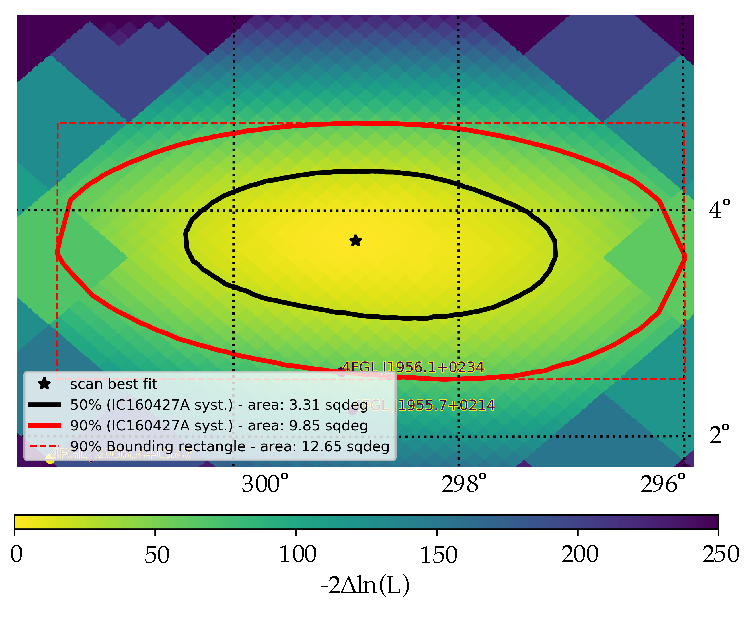
\includegraphics[width=1\textwidth]{ic/ic_millipede_IC221124A.pdf}
    \caption[\texttt{Millipede} reconstruction of \emph{IC221124A}]{\texttt{Millipede} reconstruction of \emph{IC221124A}.}
    \labfig{ic_millipede}
\end{marginfigure}

Here $T$ is the total number of knot positions, $B$ is the $i$-th basis spline of order $k$, $\vec{a}$ again describes the track, and $\kappa$ denotes the parameters of the ice model.

\subsection{\texttt{Millipede} Reconstruction}\label{millipede}

High-energy neutrino events that pass the realtime alert selection criteria (see Section~\ref{ic_alert_program}) are subjected to a more sophisticated algorithm, which uses the information from all the detected photons. This algorithm is dubbed \texttt{Millipede}. Due to its high demand of computational resources it is only run for selected events at the IceCube data center in Madison.

This reconstruction consists of a maximum likelihood scan covering the whole sky. To allow scanning, the sky is pixelated into grids of increasing resolution following the Hierarchical Equal Area isoLatitude Pixelation (\texttt{HEALPix}) scheme~\sidecite{Gorski2005}. Each pixel of a specific resolution covers the same area on the sky. For each scanned pixel, the muon direction is fixed to originate from that sky location.

For this fixed direction, the likelihood of the deposited energy resulting from the best fit and the neutrino interaction vertex in the detector are then computed. Pixels near the likelihood maximum are then subdivided with a finer \texttt{HEALPix} resolution. This procedure ultimately results in a likelihood map of the sky, with increasing granularity towards the global maximum~\sidecite{Abbasi2023}.

To compute the \SI{50}{\percent} and \SI{90}{\percent} confidence level uncertainty contours, Monte Carlo resimulations from the high-energy neutrino event \emph{IC160427A} are used. For this event, Pan-STARRS found a possible counterpart, \emph{PS16cgx}\sidenote{Spectroscopic follow up reveiled that this event was either a SN Ic, which would be compatible with neutrino production, or --- more likely --- a SN Ia, which would exclude it as a neutrino source.}~\sidecite{Kankare2019}.

In the resimulations, the systematic parameters of the Antarctic ice used to model photon propagation were varied. Additionally, the simulated direction and energies were varied, with cuts to ensure that the light deposition of the resimulations resembled the original event (\SI{\pm2}{\degree} in direction, \SI{\pm20}{\percent} in deposited charge).

Each resimulated event was fit with \texttt{Millipede}. The distribution of differences between the best-fit likelihood and the ground truth of the simulated event can then be employed to convert the change in log-likelihood over the map into a confidence level.

Due to the systematic uncertainties, Wilk's theorem does not apply here. To account for this fact, the contours derived for individual events (which make use of the theorem) are scaled up with correction values obtained from the resimulations of \emph{IC160427A}. Then, all pixels that satisfy $\log \mathcal{L}_\text{min}-\log \mathcal{L}_\text{pixel} = -11.3$ $(-32.1)$ form the \SI{50}{\percent} (\SI{90}{\percent}) error contours. Currently, these correction values are 22.2 and 64.2 for the \SI{50}{\percent} and \SI{90}{\percent} uncertainty contours~\sidecite{Gualda2021}. In Fig.~\ref{fig:ic_millipede} these contours are displayed for an example event. The black line shows the \SI{50}{\percent} uncertainty region, while the red line shows the \SI{90}{\percent} area.

However, resimulations of newer high-energy neutrino events have shown that the method of scaling up the errors with correction values obtained from resimulating \emph{IC160427A} does in some cases not faithfully capture the errors of those newer resimulations: They are sometimes under-, sometimes overestimated, depending on the topography of the event. For details on this, see~\cite{Gualda2021}.

\section{The Realtime Alert Program}\label{ic_alert_program}
Since 2016, IceCube hosts a realtime alert program, providing the astrophysical community with low-latency, high-quality astrophysical neutrino alerts~\cite{Aartsen2017a}. This program saw a major revision in 2019, when two new alert streams, named `Gold' and `Bronze', were created~\sidecite{Blaufuss2019}. As these are designed based on cuts reducing the IceCube background, one needs to understand the background events first.

\subsection{Background}\label{background}

When searching for the sources of astrophysical neutrinos, there are two major sources of background events in the IceCube detector. Both stem from secondary cosmic-ray particles from the Earth's atmosphere.

\begin{figure}[htb]
    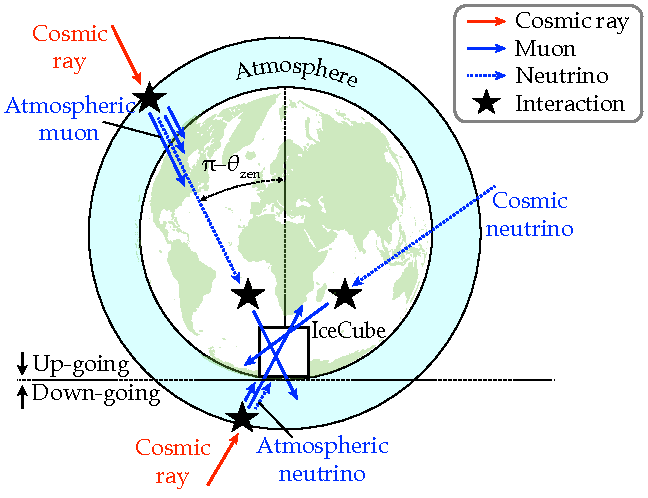
\includegraphics[width=0.8\textwidth]{ic/ic_background.pdf}
    \caption[Background events]{Background events in the detector. Cosmic rays hit the atmosphere around the globe and produce muons (solid blue arrows), as well as neutrinos (dashed blue arrows). When constraining to \textit{up-going} events from the northern hemisphere, the detector is shielded from atmospheric muons, but not atmospheric neutrinos, as these can traverse the Earth. Adapted from~\cite{Ahlers2018a}.}
    \labfig{ic_background}
\end{figure}

\begin{marginfigure}
    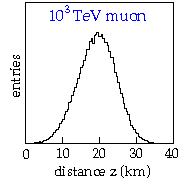
\includegraphics[width=0.8\textwidth]{ic/ic_muon_free_path.pdf}
    \caption[Muon free path in ice]{Free path length for \SI{1}{\peta\eV} muons in ice. The mean free path in ice is slightly longer than in rock. From~\cite{Chirkin2004}.}
    \labfig{ic_muon_free_path}
\end{marginfigure}

\begin{description}
    \item[Atmospheric Muons] are created by cosmic rays hitting the atmosphere. One can efficiently filter this background by restricting the analysis to \textit{up-going} muon tracks. These are tracks that come from the bottom of the detector, i.e.\ the northern hemisphere. Atmospheric muons stemming from cosmic-ray events in the northern hemisphere are filtered out by the Earth's core (see Fig.~\ref{fig:ic_background}), as the mean free path of muons within the Earth is much smaller~\sidecite{Chirkin2004} than the distance they have to cross (see Fig.~\ref{fig:ic_muon_free_path}). Note that due to light scattering within the ice, some down-going tracks can be misclassified as up-going~\sidecite{Ahlers2018a}.

          One complication here stems from the fact that the Earth starts to become opaque for neutrinos of higher energies. Studies interested in \si{\peta\eV} neutrinos therefore must deal with the fact that these get the more suppressed the longer their path through the Earth is. For example, a \SI{1}{\peta\eV} neutrino with a zenith angle of \SI{140}{\degree} is absorbed with \SI{90}{\percent} probability~\sidecite{Aartsen2017c}.

          \begin{figure}[htb]
              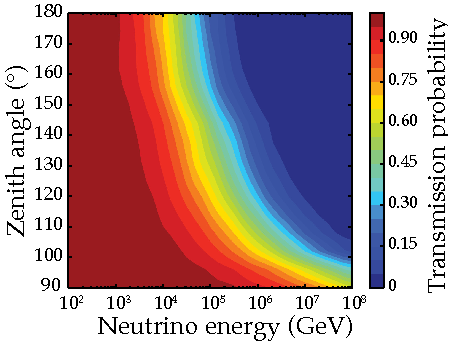
\includegraphics[width=0.5\textwidth]{ic/ic_absorption_earth.pdf}
              \caption[Neutrino absorption in the Earth]{Neutrino transmission probability through the Earth. The longer the distance traveled (higher zenith angles) and the higher the neutrino energy, the more likely is absorption. From~\cite{Aartsen2017c}.}
              \labfig{ic_absorption_earth}
          \end{figure}

    \item[Atmospheric Neutrinos] also stem from cosmic-ray induced air showers. These cannot be suppressed by directional cuts, creating an irreducible background: When atmospheric neutrinos cross the Earth and interact with the matter close to the detector, they can produce muons indistinguishable from muons created by `proper' cosmic neutrinos~\cite{Ahlers2018a}.

\end{description}

\subsection{Event Selection}\label{ic_event_selection}

Gold and Bronze alerts are drawn from three different selection schemes, originally designed to cater to different science goals. These are High Energy Starting Events (HESE)~\sidecite{Abbasi2021}, Extremely High Energy (EHE) events~\sidecite{Aartsen2016} and Gamma-Ray Follow Up (GFU) events~\sidecite{gfu2016}.

\begin{description}

    \item[HESE] are events that start \textit{within} the detector. This is guaranteed by using the outer regions of the detector as a veto region, in which (almost) no Cherenkov light must be detected~\cite{Aartsen2013}. The sizes of those regions can be seen in Fig.~\ref{fig:ic_hese_veto}. The majority of HESE events are cascade-type events and therefore not well suited for observational follow-up due to their poor angular reconstruction. Because of this drawback, additional cuts are applied: At least 6000 photoelectrons are required, and the reconstruction must favor a track interpretation of the event, and the reconstructed track length must be at least \SI{200}{\meter}~\cite{Abbasi2023}. Note that the selection criteria used in the Gold and Bronze HESE selection are slightly different than those in the original paper cited above.

    \item[EHE] aims at neutrino energies of \SIrange{0.5}{10}{\peta\eV}. To reject atmospheric background events, a two-dimensional cut depending on the reconstructed zenith angle and the log of detected photoelectrons is applied. Additionally, a $\chi^2$-based goodness-of-fit cut is applied to select track-like events with good reconstructions~\cite{Abbasi2023}.

          \begin{marginfigure}
              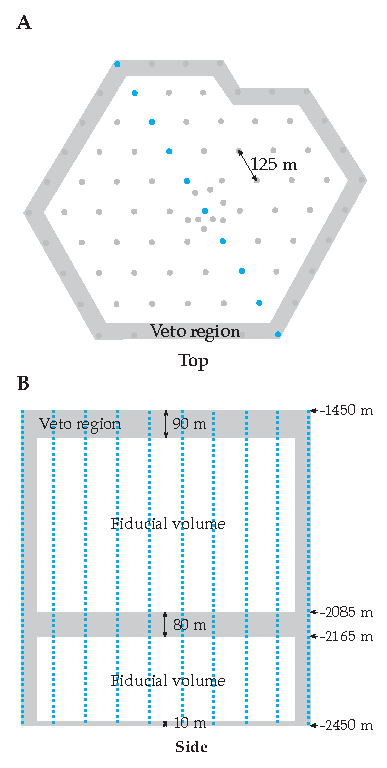
\includegraphics{ic/ic_HESE_veto.pdf}
              \caption[HESE veto regions]{High-energy starting events veto regions. The strings marked in blue in the top-down view at the top (A) show the location of the side view, displayed at the bottom (B). From~\cite{Aartsen2013}.}
              \labfig{ic_hese_veto}
          \end{marginfigure}

    \item[GFU] events are selected based on a boosted decision tree trained to identify \textit{through-going} (as opposed to `starting') track events with astrophysical origin. Energy cuts are applied: Northern hemisphere events are selected based on their reconstructed muon energies, while from the southern hemisphere are selected based on the total photoelectron charge deposited in the detector.
\end{description}

The cuts from all three event pools are gauged to achieve two different average values of signalness, which is a proxy for the probability that the event is of astrophysical origin~\cite{Abbasi2023}. It is defined as
\begin{definition}\label{signalness_def}
    $\text{Signalness}(E,\theta_\text{zen}) = \frac{N_\text{signal}(E,\theta_\text{zen})}{N_\text{signal}(E,\theta_\text{zen})+N_\text{background}(E,\theta_\text{zen})}$
\end{definition}
Here E is the reconstructed neutrino energy, and $N_\text{signal}(E,\theta_\text{zen})$ and $N_\text{background}(E,\theta_\text{zen})$ are the number of signal and background events at zenith angle $\theta_\text{zen}$ above energy $E$ as determined by simulations~\cite{Abbasi2023}.

The cuts on the individual event selections are tuned to ensure that \textit{Gold} alerts on average have a signalness $\langle \SI{50}{\percent} \rangle$, and \textit{Bronze} alerts have a signalness $\langle \SI{30}{\percent} \rangle$.

\subsection{Alert Distribution} \label{ic_alerts}
All events that pass a first stage of filtering are sent to the IceCube data center (see Section~\ref{data_acquisition}) via Iridium satellite to minimize latency. There, their signalness is computed. After this, they are globally distributed with the General Coordinates Network\sidenote{\url{https://gcn.nasa.gov/}} (GCN) in the form of GCN Notices.

Each notice contains the discovery time, a unique event number, the reconstructed direction in right ascension (RA) and declination (Dec) of the candidate neutrino computed by \texttt{SplineMPE}\sidenote{See Section~\ref{spline_mpe}.}, a statistical error for the direction, the reconstructed neutrino energy, the signalness and the false alarm rate~\cite{Blaufuss2019}.

\begin{marginfigure}
    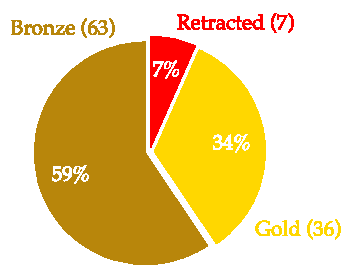
\includegraphics{ic/ic_he_alert_overview.pdf}
    \caption[IceCube alert overview]{High-energy neutrino alerts issued by IceCube since start of the new alert stream in June 2019.}
    \labfig{ic_he_alert_overview}
\end{marginfigure}

Those informations are later appended by \texttt{Millipede}, a computationally more demanding, but more sophisticated reconstruction (see Section~\ref{millipede}). The results of these reconstructions (i.e.\ the angular uncertainty) are typically distributed a few hours after the initial notice in the form of a GCN circular, and an updated GCN notice~\cite{Blaufuss2019}.

As of March 2023, a total of 106 events have been distributed in this format, with 7 later being retracted. Since the start of the Gold and Bronze alert stream in June 2019, this amounts to 2.2 non-retracted alerts per month\sidenote{This is quite close to the 2.5 alerts per month predicted in~\cite{Blaufuss2019}.} (0.8 Gold alerts, 1.4 Bronze alerts). For a full list of all high-energy neutrino alerts issued by IceCube, not only those since introduction of the Gold and Bronze format, see~\cite{Abbasi2023}.

If the event is most likely astrophysical and reasonably well pin-pointed, one can scan the sky localization with a telescope and look for potential sources of the neutrino. But where to obtain optical images from? The telescope used for this, the Zwicky Transient Facility, will be described in Chapter~\ref{ztf}.




\setchapterimage[7cm]{ztf/ztf_telescope.png}
\chapter{The Zwicky Transient Facility} \label{ztf}
\labch{ZTF}
The second instrument relevant for this thesis is the Zwicky Transient Facility (ZTF). It is named after the notorious Swiss-American astronomer Fritz Zwicky\sidenote{He first employed the Virial theorem to infer the existence of dark matter \cite{Zwicky1933}. Furthermore, together with Walter Baade, he posited the existence of supernovae and the creation of neutron stars in such events \cite{Baade1934}.}.

ZTF is a wide-field optical survey telescope. Its wide field means that its use case is to periodically scan the full sky, in contrast to getting pictures of specific objects. As its angular resolution is poor, ZTF is most sensitive to changes in brightness and therefore to the detection of transient events (short: \textit{transients}).\sidenote{Transient astrophysical events are observed as the time evolution of flux at different wavelengths from a small region on the sky.}

 ZTF is located at Mount Palomar in California, United States, at \SI{1700}{\m} above sea level, roughly \SI{130}{\km} southeast of Los Angeles. Its optical system, the \SI{1.2}{\m} (48 inch) Samuel Oschin telescope, follows a Schmidt design (see below\todo{Section}) and was inaugurated in 1948 \cite{Harrington1952}. At first light and for years to come, it was the largest Schmidt telescope in the world. Originally, the telescope exposed photographic plates, covering a field of view (FoV) of \SI{44}{\square\deg}. As such photographic plates have obvious drawbacks, and because technological progress made it possible, the Near-Earth Asteroid Tracking (NEAT) program \sidecite{Pravdo1999} replaced them with a charge-coupled device (CCD) camera in the early 2000s.\marginnote{See \url{https://sites.astro.caltech.edu/palomar/about/telescopes/oschin.html} for a historical overview.}

During the following years, the camera was updated several times\todo{twice? how often?}. The immediate predecessor of ZTF, the Palomar Transient Factory (PTF) \sidecite{Law2009}, began operation in 2009. Equipped with a 96 Megapixel camera, it already had many of the characteristics of ZTF: A fully automated survey, searching for optical transients with a CCD camera.

ZTF follows the concept of PTF, but is equipped with a larger and more sensitive camera. With \SI{47}{\square\deg}, the 600 Megapixel camera covers the full FoV of the P48. The main design metric for ZTF was \textit{volumetric survey speed}. This is the volume within which an object of given absolute magnitude can be detected in one exposure, divided by the total time for the exposure (observation plus overhead) \sidecite{Bellm2016}. The system saw first light in 2017, and started scientific operations in 2018 (the first survey data was taken on 2018-03-20). As of writing, ZTF is still operational.

There are two other telescopes located on Mount Palomar: The \SI{1.5}{\meter} (60 inch) P60 telescope houses the SED Machine (SEDM) \sidecite{Blagorodnova2018}, a fully robotic, low-resolution spectrograph used for automatic classification of transients. The largest facility on the mountain is the 200-inch (\SI{5.1}{\meter}) Hale Telescope, which is used for optical and infrared photometry as well as mid- and high-resolution spectroscopy of fainter sources. Together, these telescopes form a natural hierarchy: ZTF is the discovery engine for optical transients. Promising sources are then classified with SEDM. If a source warrants it, deeper photometry and better resolved spectroscopy can then be obtained with the P200. All three telescopes are shown in Fig. \ref{fig:palomar_overview}.

\begin{figure*}[]
    \includegraphics{ztf/palomar_overview.pdf}
    \caption[View of Mt. Palomar]{View of Mt. Palomar with the three telescopes highlighted in the text. Image credit: Caltech, annotations by the author.}
    \labfig{palomar_overview}
\end{figure*}

\section{Telescope Design}
A \textit{Schmidt telescope} like ZTF is by design dedicated to taking images, contrary to earlier designs allowing to observe through an eyepiece \sidecite{Schmidt1938}. For this reason, it is also referred to as a \textit{Schmidt camera}. The design goal was a wide FoV. This made it the ideal instrument for sky surveys, where a large FoV maximizes the on-sky area that can be monitored. A Schmidt telescope combines a spherical mirror at the end of the telescope tube with an aspherical correcting lens (Schmidt plate) at the tube's entrance. The use of a spherical mirror combined with the correcting lens gets rid of comatic aberration\todo{zusatz oder das ist nur blabla}.

\begin{figure}[]
    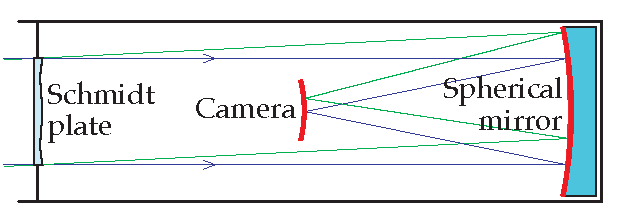
\includegraphics[width=1\textwidth]{ztf/schmidt2.pdf}
    \caption[Schmidt telescope schematic]{Schmidt telescope schematic. Light enters from the left, passes the Schmidt plate (an aspherical correcting lens), gets reflected by a spherical mirror at the end onto a photographic plate or camera halfway down the tube. Figure adapted from \url{https://commons.wikimedia.org/wiki/File:Schmidt-Teleskop.svg}.}
    \labfig{schmidt_telescope}
\end{figure}

Until the end of the 20th century, around ten Schmidt telescopes have been built, most of them to conduct sky surveys \sidecite{Cannon1995}. At least two of them were space telescopes: ESA's astrometry mission \textit{HIPPARCOS} \sidecite{ESA1997} (1989--1993) and the NASA explanet mission \textit{Kepler} \sidecite{Koch2010} (2009--2018). In both cases, the mission entailed monitoring of large areas of the sky; prime territory for Schmidt telescopes.

\begin{figure}[]
    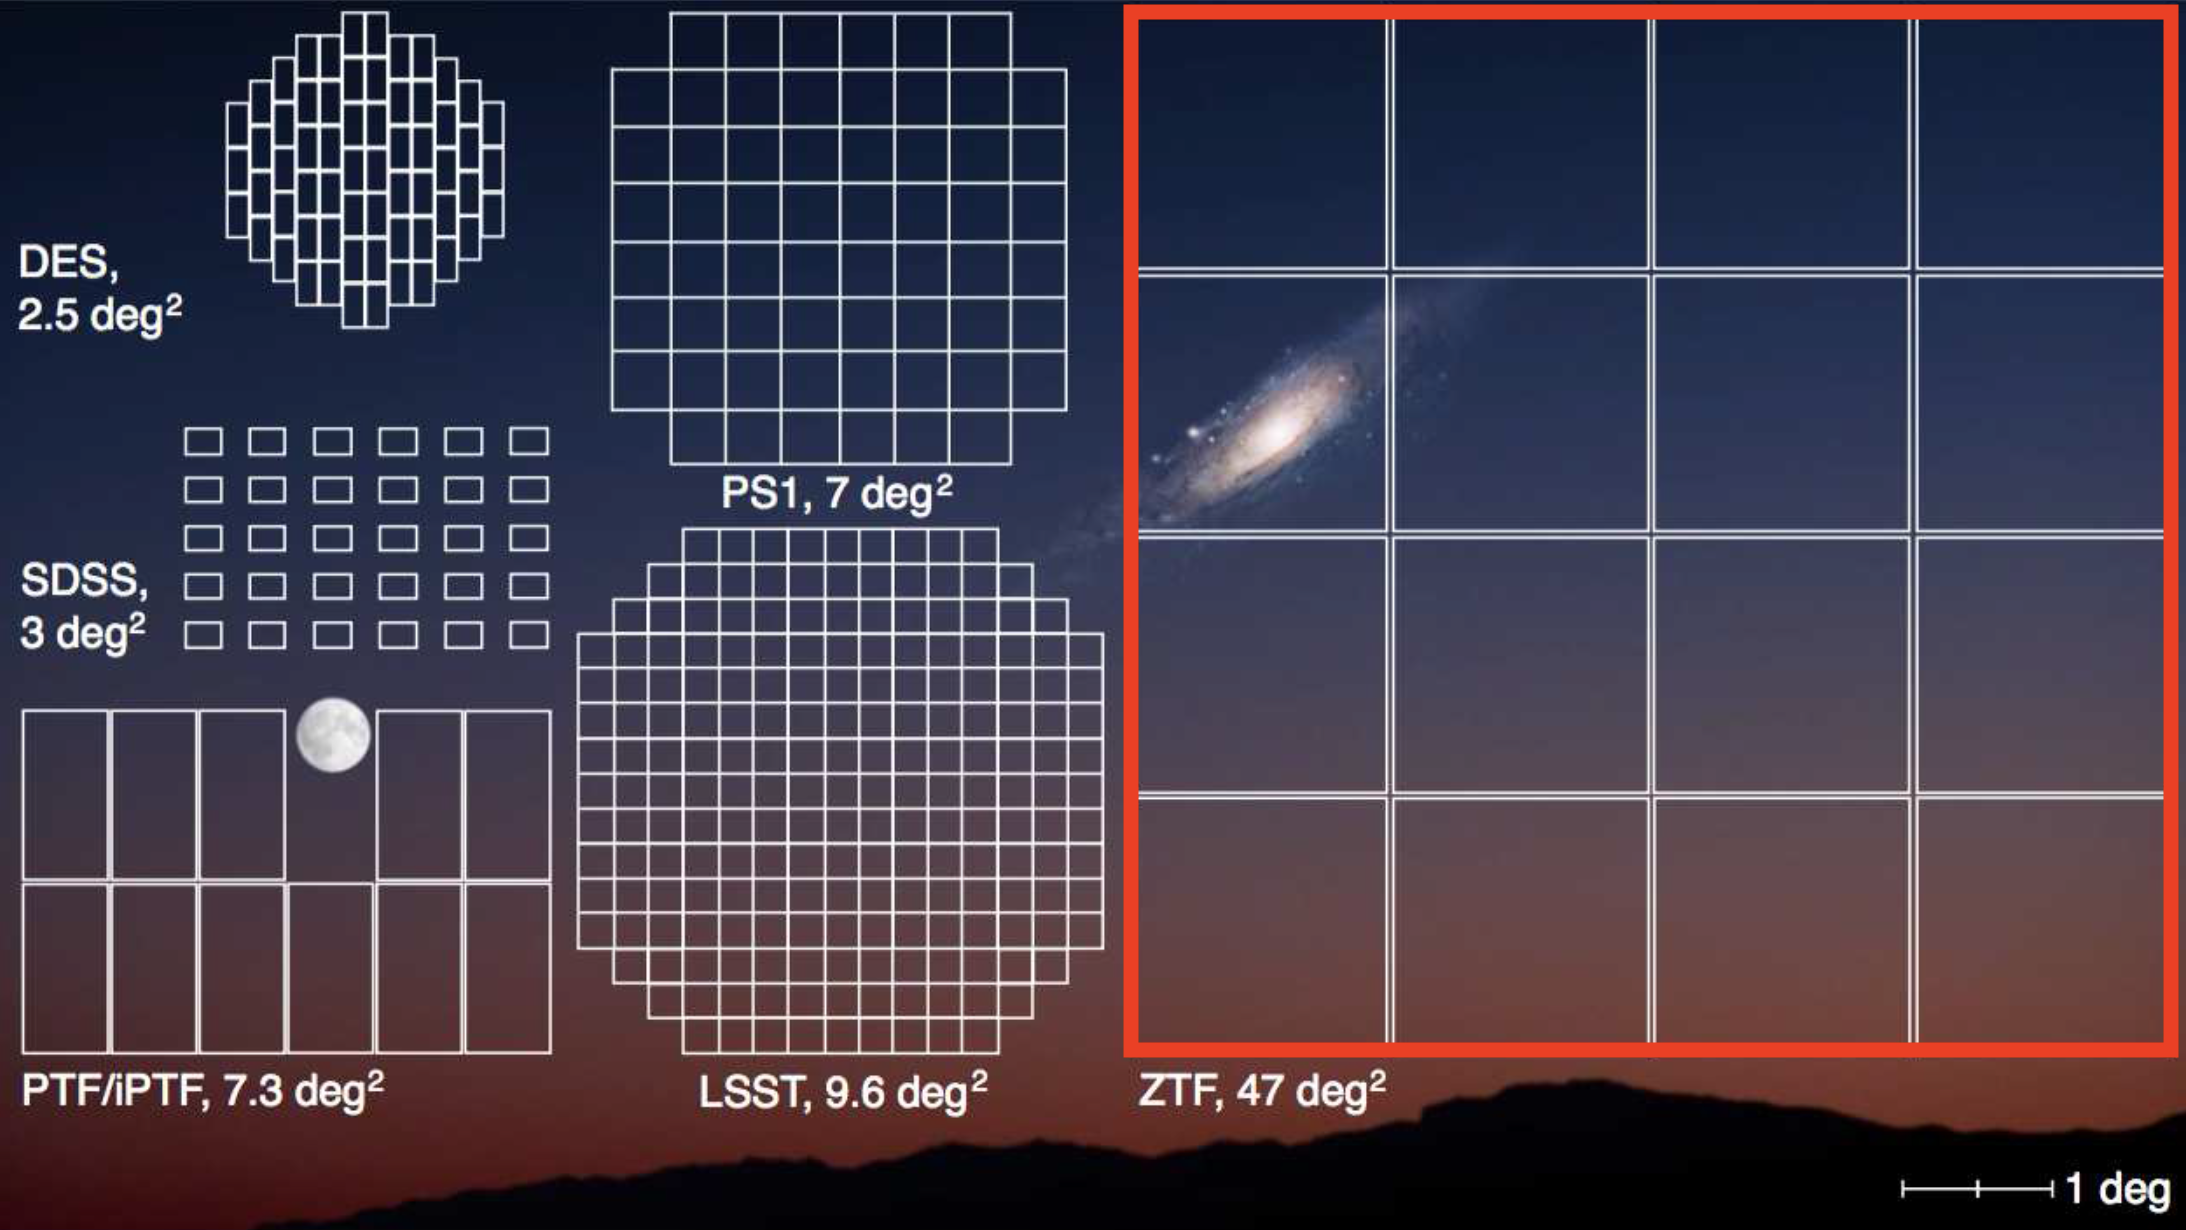
\includegraphics[width=1\textwidth]{ztf/ztf_fov.pdf}
    \caption[ZTF Field of View]{ZTF field of view (highlighted in red) in comparison to other sky survey telescopes, including the future Rubin observatory (LSST) \cite{Ivezic2019}. Note also the 6.5-fold increase with respect to ZTF's predecessor, PTF/iPTF. From \cite{Laher2018}, highlighting by the author.}
    \labfig{ztf_fov}
\end{figure}



\section{Camera}
\begin{marginfigure}
    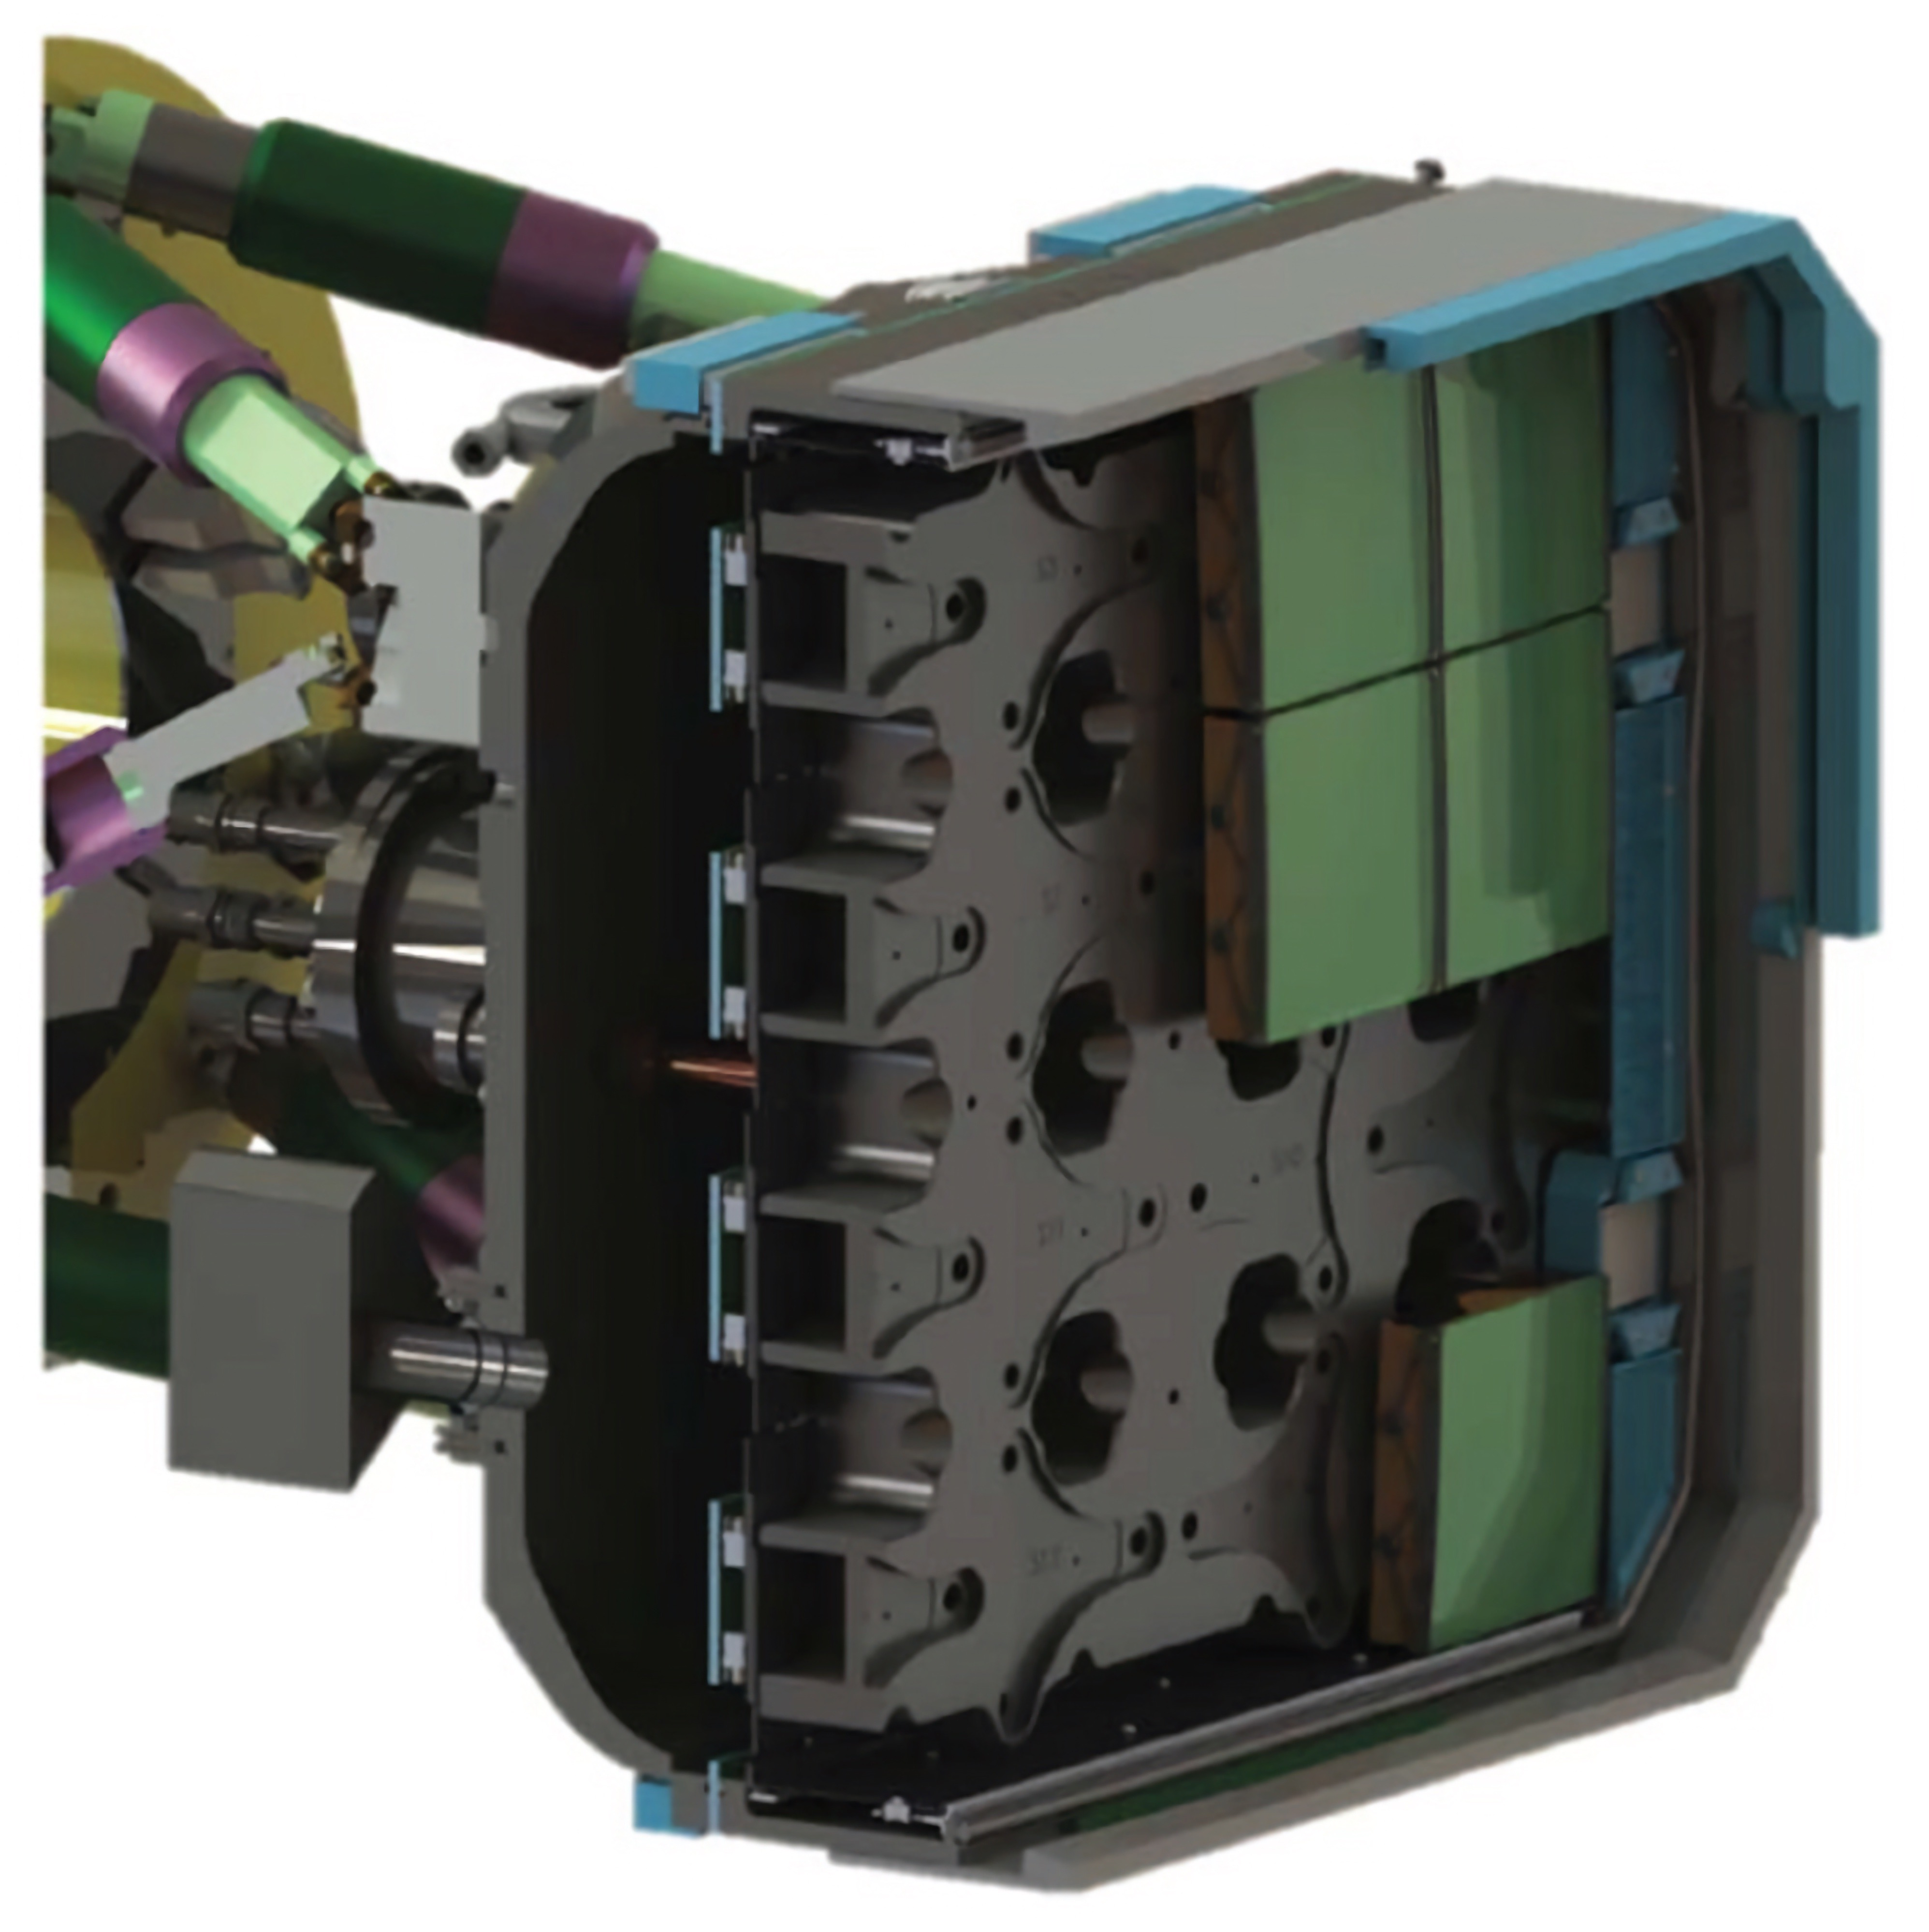
\includegraphics{ztf/ztf_camera_detail_highres.jpg}
    \caption[ZTF camera cutaway]{The ZTF camera in detail. From \cite{Dekany2020}.}
    \labfig{ztf_camera_detail}
\end{marginfigure}
The ZTF camera is a CCD design, consisting of 16 individual CCDs by commercial manufacturer e2v (now Teledyne, \textit{Science CCD231-C6}), each having 6144x6160 pixels, resulting in a total camera resolution of $\sim 600 \,\textrm{Megapixel}$ \sidecite{Dekany2016}. As one can see in Fig. \ref{fig:ztf_camera}, the array of 16 CCDs is slightly bent. This is necessitated by the Schmidt design, where the camera needs to be spherical, matching the spherical mirror. As individual CCDs are flat, each of the 16 sensors is is installed slightly tilted, tracing the overall curvature. To get rid of residual deviations from the global curvature, in front of each sensor a field flattener lens is mounted \sidecite{Bellm2019}.

\begin{marginfigure}
    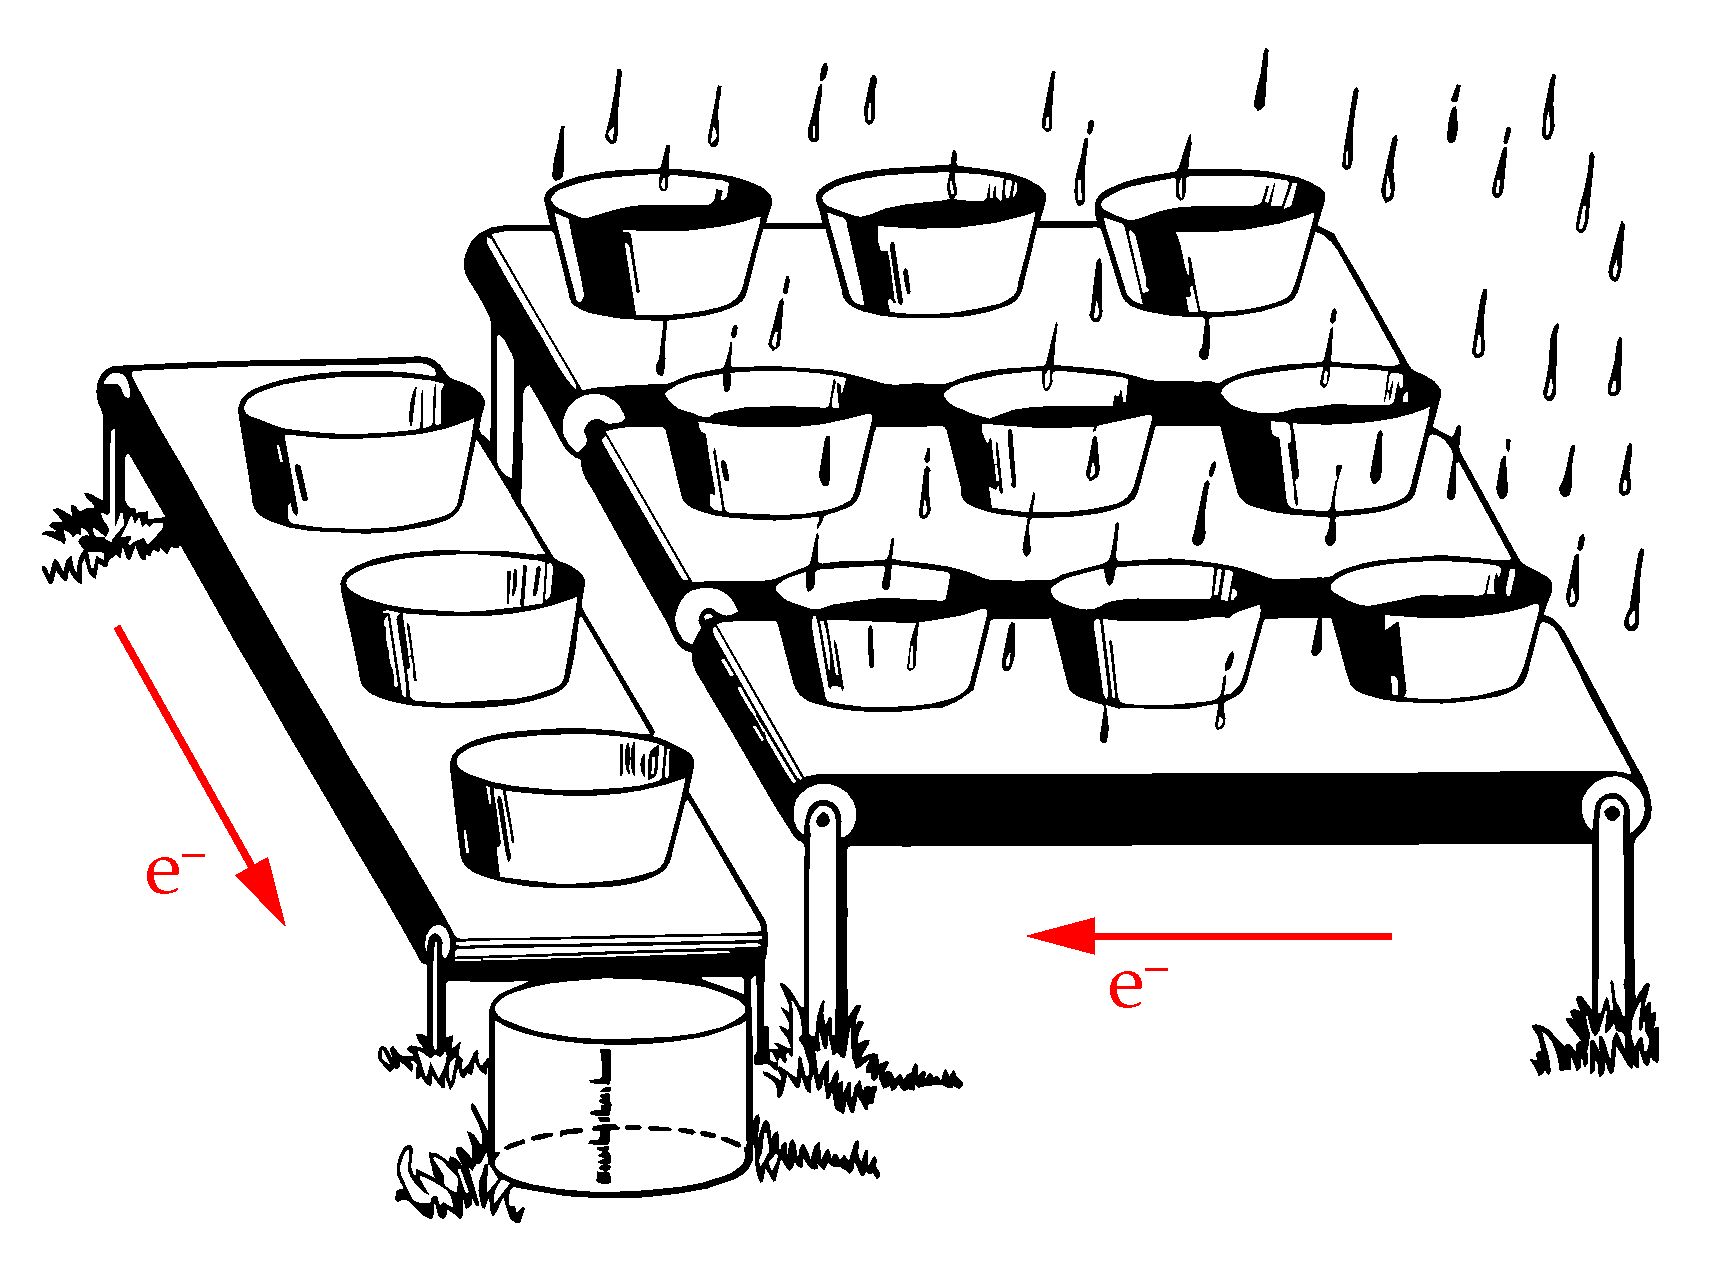
\includegraphics{ztf/ccd_buckets.pdf}
    \caption[CCD operational principle]{CCD operational principle, explained with buckets measuring precipitation. From \cite{Janesick1987}.}
    \labfig{ccd_buckets}
\end{marginfigure}

\subsection{CCDs}
CCDs are silicon-based light sensors. They consist of arrays of coupled metal-oxide semiconductor (MOS) capacitors. Each one these is able to store the charge created by incident photons; spatial resolution is achieved by having one capacitor per pixel of the sensor array. The array is then exposed to light for a specified amount of time (exposure time). During the exposure, incident photons create a charge proportional to the amount of light hitting each capacitor via the photo-electric effect. This charge is accumulated in each capacitor until the exposure is finished. To read out the CCD, the charges need to be moved to neighboring capacitors. When the MOS capacitors are tightly placed, one can move the charges from one capacitor to the next by changing the voltages on the capacitor's gates.

In Fig. \ref{fig:ccd_buckets} the principle of a CCD is explained with little buckets collecting rain water. Each bucket symbolizes one capacitor or one pixel of the sensor array respectively. After the rain has stopped (the exposure is finished), each bucket naturally contains an amount of water proportional to the amount of water that rained down over it. Now the amount of water in each bucket (the charge deposited by incident light in each capacitor) needs to be measured.

To do this, the buckets in each row are moved one position to the left with horicontal conveyor belts. Each bucket at the left end of the horicontal conveyor belt is then emptied into the bucket on the single vertical conveyor belt. The buckets of this vertical belt are then one by one drained into the meausuring bucket on the bottom left. After all buckets on the vertical belt are emptied, the process starts anew, until all buckets are empty. As one can see, the time this process takes is quadratic to the amount of buckets (or pixels) \sidecite{Janesick1987}. To speed up the process, one can subdivide the sensor area into smaller sections, which are read out in parallel.

Each CCD pixel actually consists of three electrodes, which can be seen in Fig. \ref{fig:ccd_transport}. The transport of charge within the CCD is realized by subsequently applying a higher voltage to different electrodes, moving the charge step-wise. 

\begin{figure}[htb]
    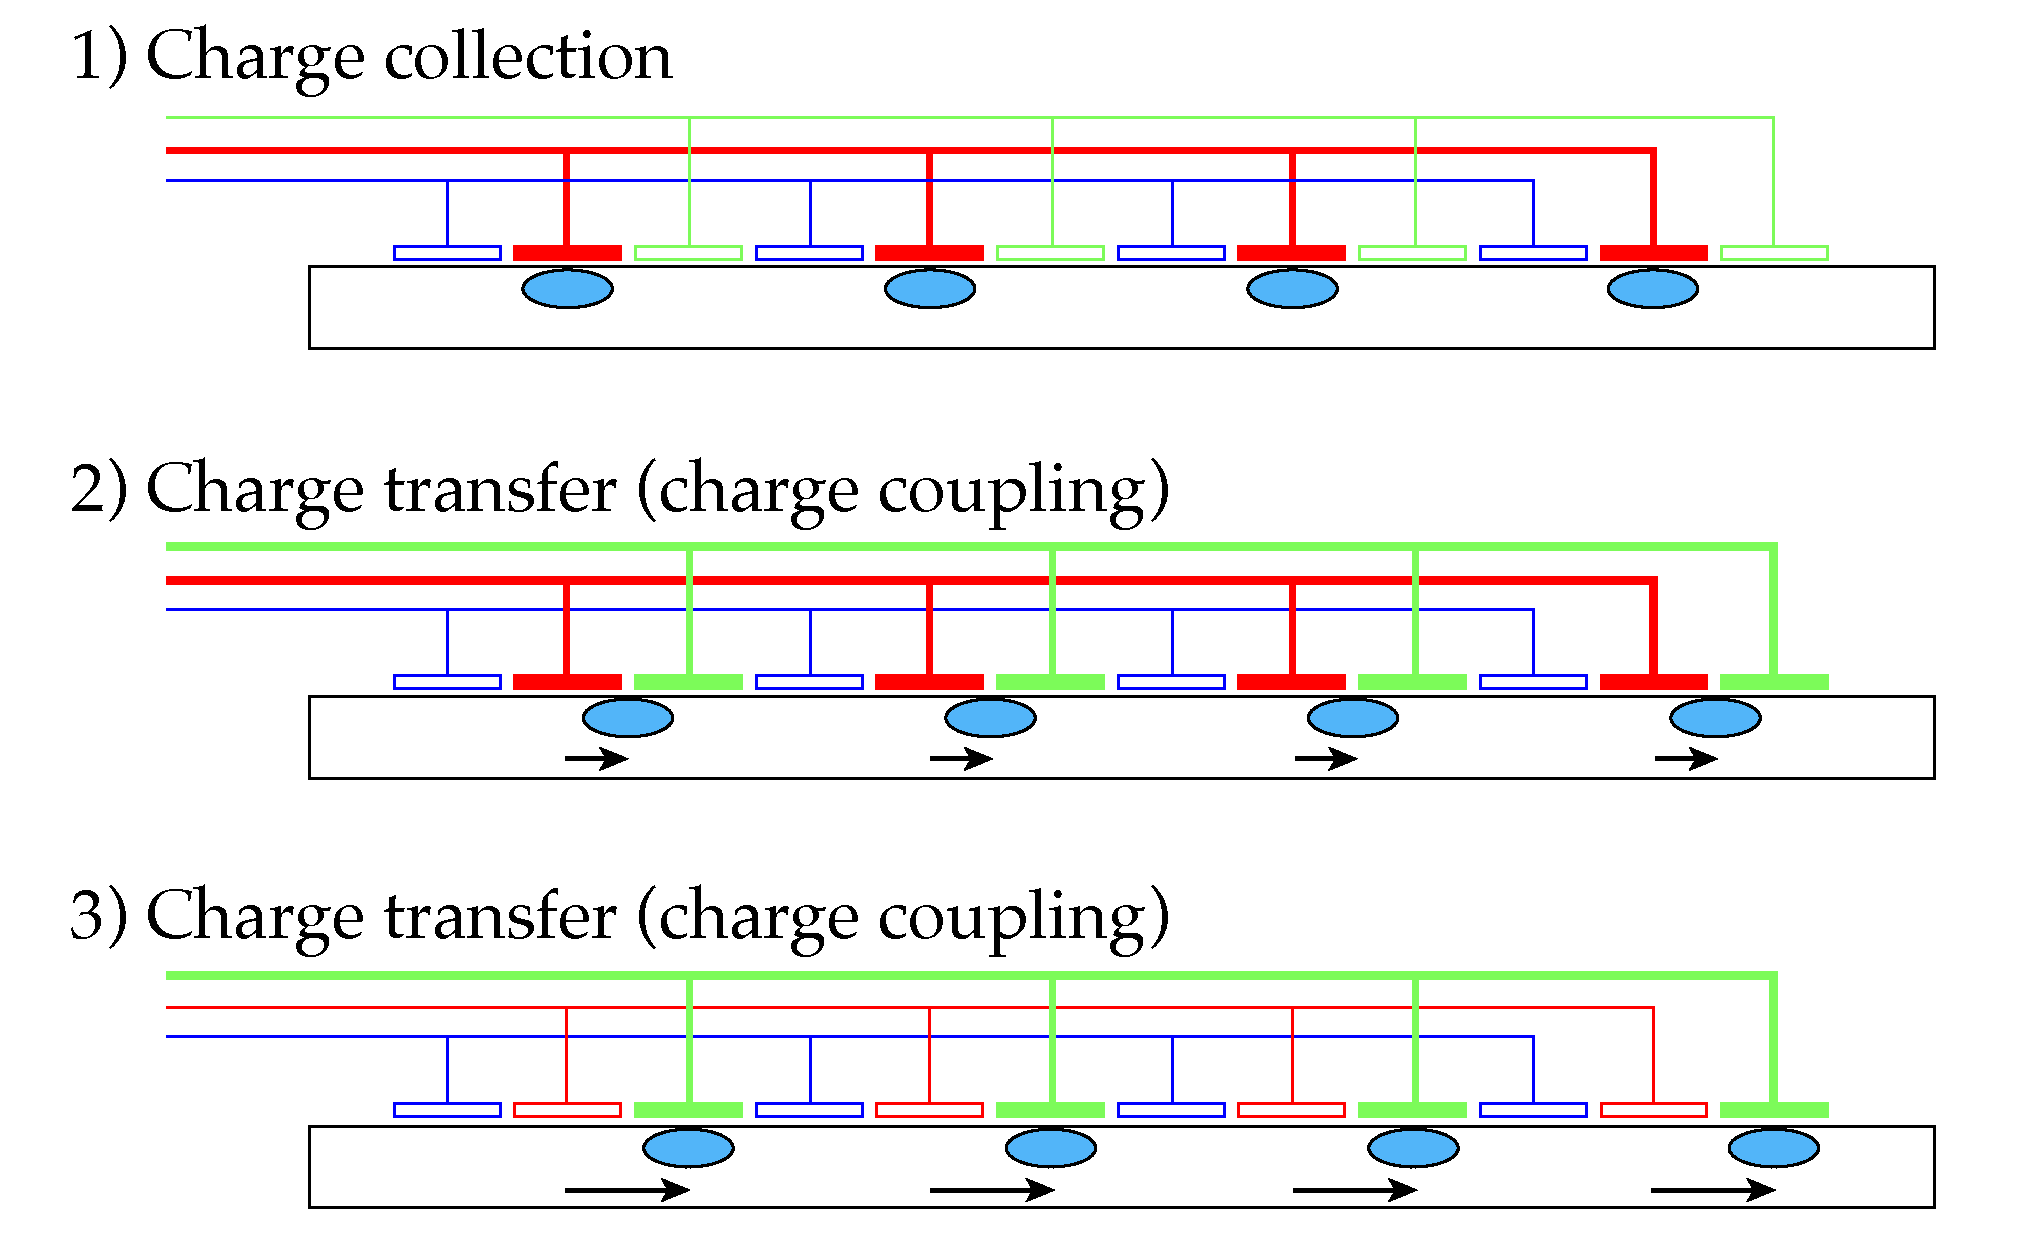
\includegraphics[width=0.7\textwidth]{ztf/ccd_transport.pdf}
    \caption[Charge transport in a CCD]{Charge transport in a CCD. High voltage electrodes are shown filled, while low voltage electrodes are empty. By stepping through different combinations of electrodes, the electric potential changes, and the charge moves.}
    \labfig{ccd_transport}
\end{figure}

The typical exposure for the ZTF camera is \SI{30}{\second}, while the readout time (transferring and measuring the charge in each capacitor) is \SI{8.2}{\second}. Readout and digitization is done in parallel for four quadrants, each containing 4 CCDs. The four readout devices for the quadrants are \textit{Archon} CCD controllers by Semiconductor Technology Associates (STA), operated at \SI{1}{\mega\Hz}. Each of these operates 16 simultaneous readout channels, four for each CCD. In total, the camera is simultaneously read out in 64 independent regions to speed up the process.

Four additional smaller CCDs (2k x 2k pixels) are used as guidance, tip, tilt and focus sensors, with one additional Archon controller to read them out \sidecite{Dekany2020}. To reduce the thermal noise of the camera, it was placed on a cold plate, which is cooled by a cryocooler to \SI{160}{\kelvin} \cite{Dekany2016}.

\begin{figure}[htb]
    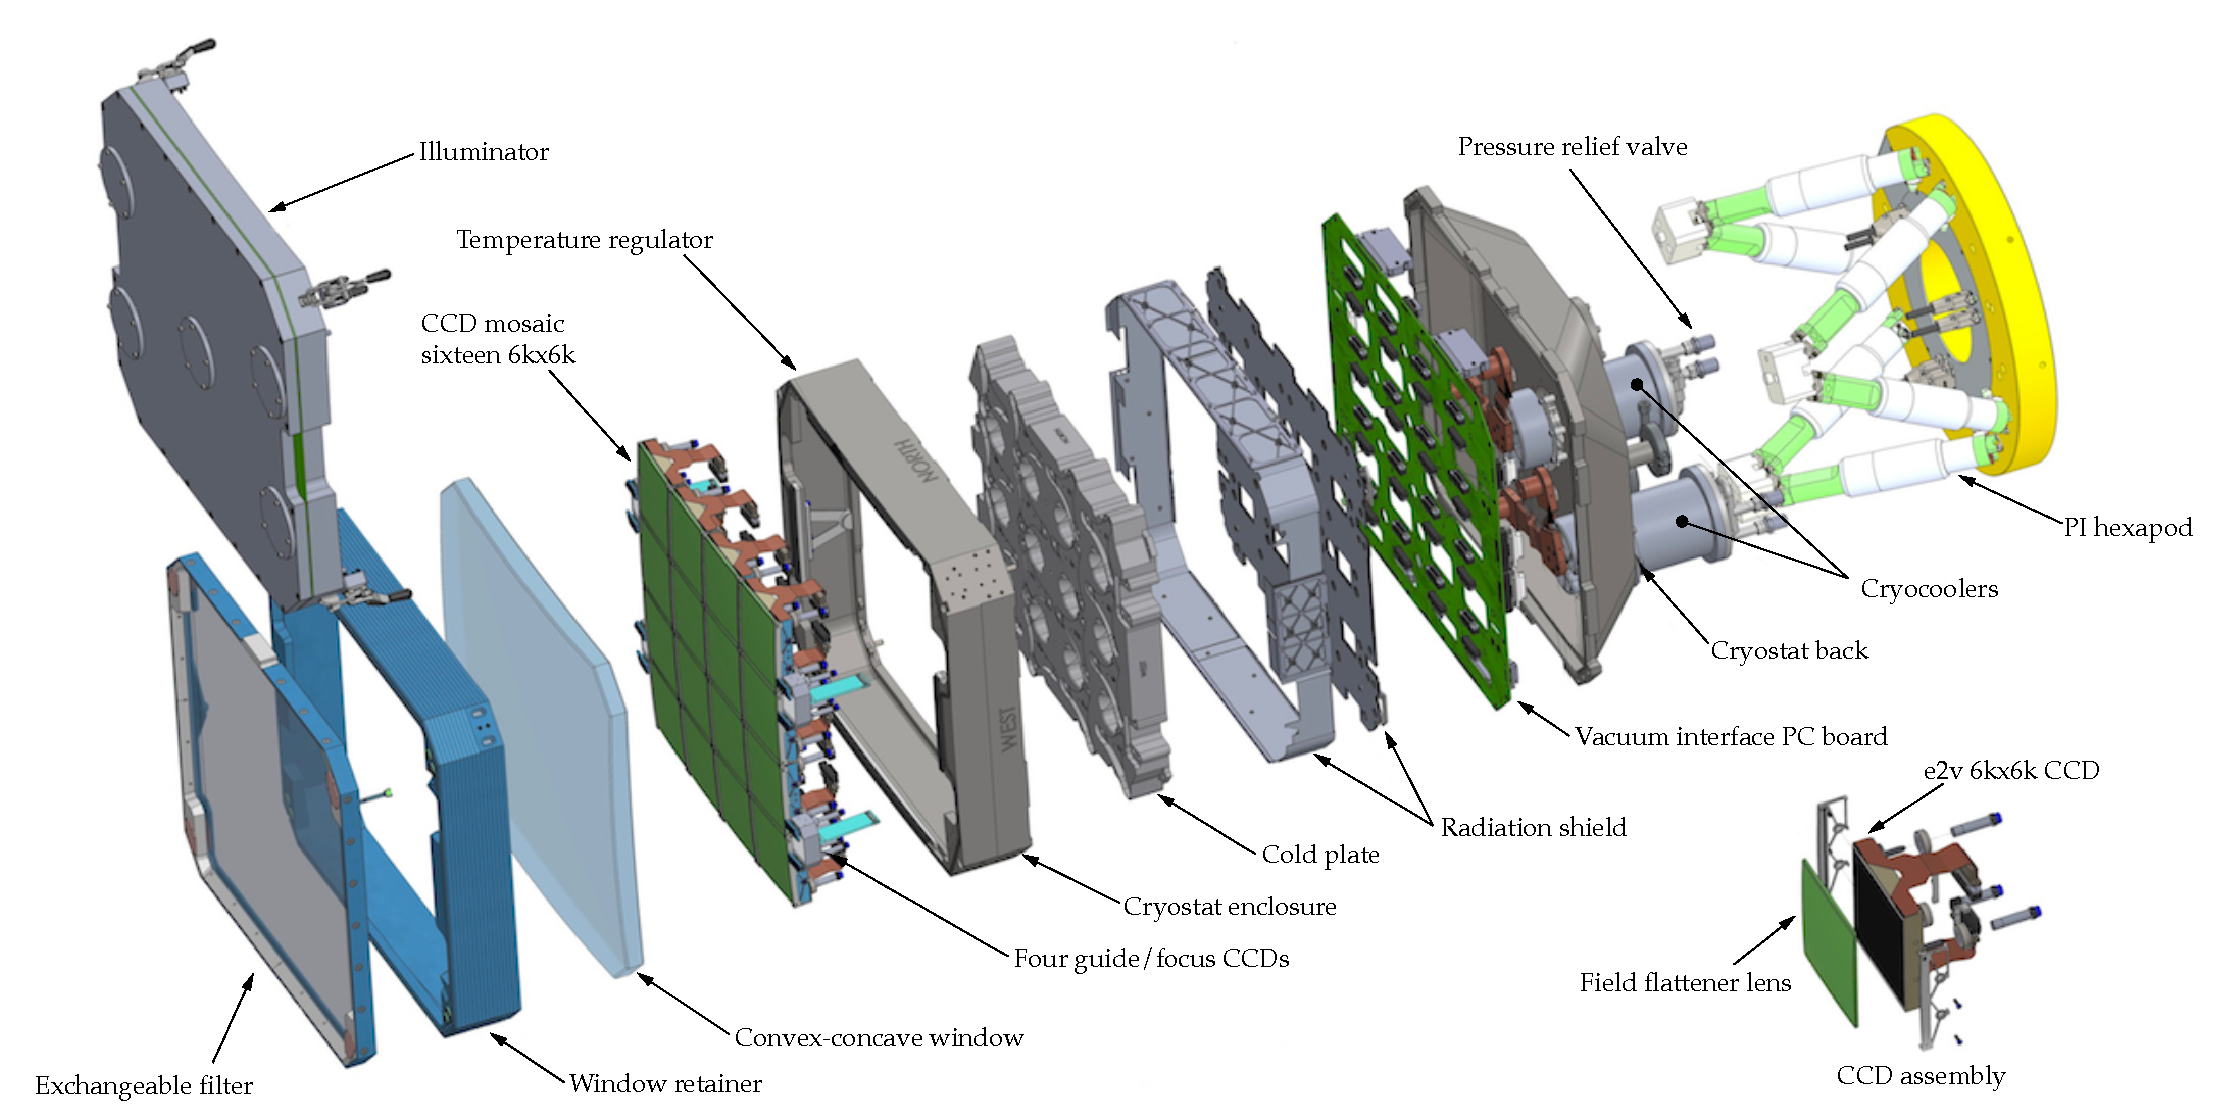
\includegraphics[width=1\textwidth]{ztf/ztf_camera.pdf}
    \caption[ZTF camera]{The ZTF camera. One can see the CCDs sandwiched between the filter on the front and the cryostat on the back. From \cite{Bellm2019}.}
    \labfig{ztf_camera}
\end{figure}

\section{Optical System}

\subsection{Filters and shutter}
As the CCDs of the camera cannot ``see'' color, different filters must be placed in front of the camera. Color information can then be obtained by imaging the object in question with a least two filters. ZTF employs three different filters: A \textit{g}-band filter with a median wavelength of \SI{472}{\nano \meter} (corresponding to blue light), an \textit{r}-band filter (median wavelength: \SI{634}{\nano \meter}, red light) and an \textit{i}-band filter (\SI{789}{\nano \meter}, near-infrared). These filters can be exchanged with a robotic arm, securely stowing the replaced filter and magnetically attaching the new one \cite{Dekany2020}; a process taking \SI{110}{\second} \cite{Bellm2019}. 

The main decision goal for the filter selection was to maximize the signal-to-noise ratio by avoiding major sky emission lines at Mt. Palomar while avoiding excessive costs. ZTF does not exactly match the filters of potential calibrators, e.g. the Sloan Digital Sky Survey (SDSS) \sidecite{York2000}, PanSTARRS (PS1) \sidecite{Kaiser2002} or \textit{Gaia} \sidecite{Prusti2016}. This was justified with the overall different telescope design of ZTF \cite{Bellm2019}.

\begin{marginfigure}
    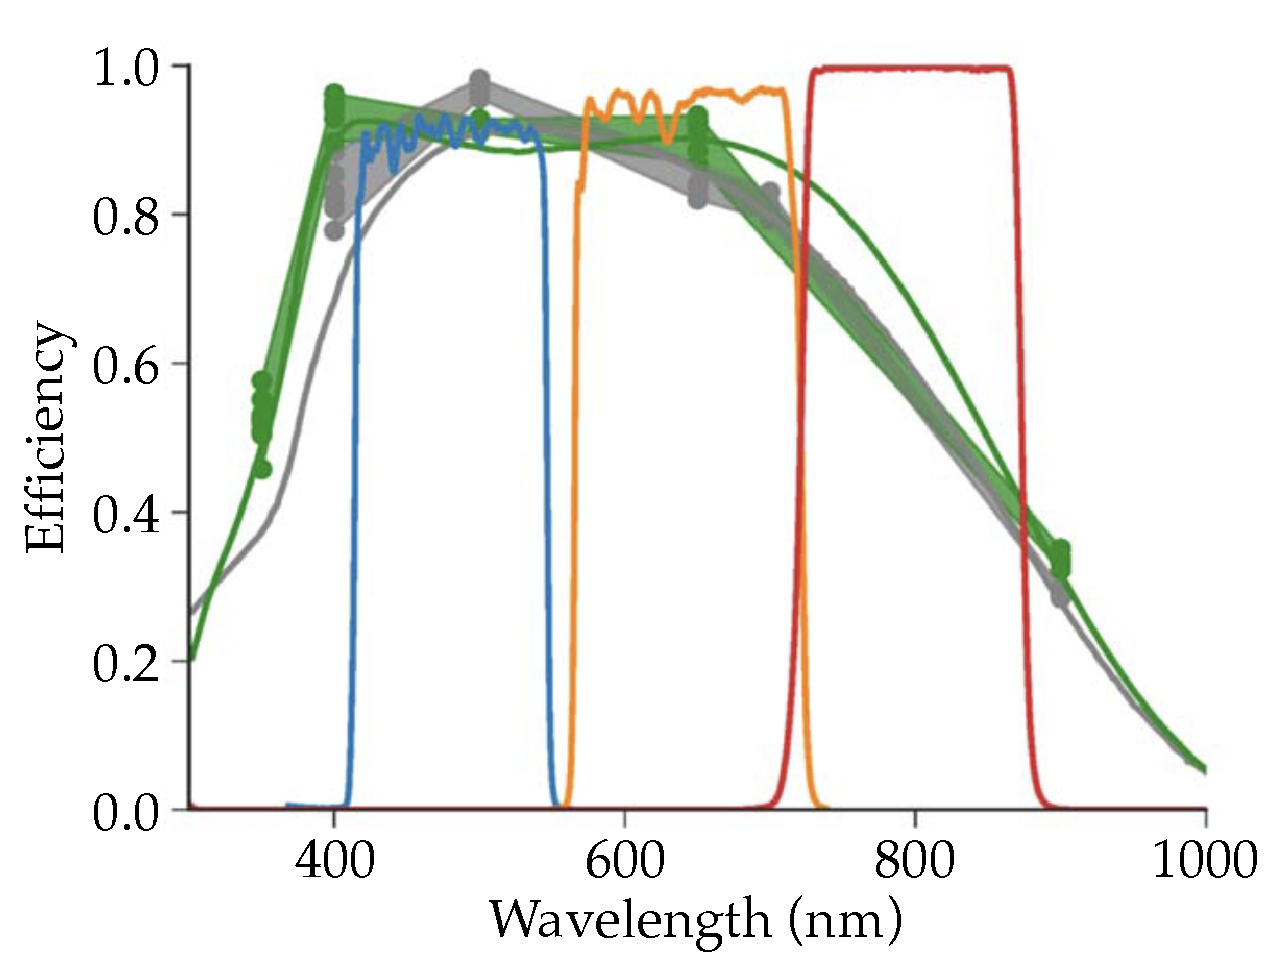
\includegraphics{ztf/ztf_throughput.pdf}
    \caption[ZTF filter transmission]{ZTF filter transmission for the three different bands (\textit{g}-band: blue, \textit{r}-band: orange, \textit{i}-band: red). The green and gray datapoints show the CCD quantum efficiency measurements (single and double-layer reflective coating). From \cite{Bellm2019}.}
    \labfig{ztf_transmission}
\end{marginfigure}

The transmission of each filter and the CCD quantum efficiency curve can be seen in Fig. \ref{fig:ztf_transmission}. As one can see, the quantum efficiency starts to decrease within the \textit{r}-band towards higher wavelengths, rendering the \textit{i}-band the least sensitive of the three filters. The $5\sigma$ median sensitivity for a 30s exposure reflects that fact. It is 20.8 (21.1) mag in the \textit{g}-band, 20.6 (20.9) mag in the \textit{r}-band and 19.9 (20.2) mag in the \textit{i}-band; with values for optimal conditions (new moon) in brackets. The resulting median image quality is 2.1'' (\textit{g}-band), 2.0'' (\textit{r}-band) and 2.1'' full width at half maximum (FWHM) of the point spread function (PSF, see Section \ref{psfphot} below) \cite{Bellm2019}.

To decrease light obstruction, the ZTF shutter was newly developed and is mounted in front of the aperture, outside of the telescope tube. It was developed by Deutsches Elektronen-Synchrotron (DESY) in cooperation with industry partner Bonn-Shutter and allows to open and close in \SI{290}{\milli \second} \cite{Dekany2020}.

\subsection{ZTF grid} \label{ztf_grid}
One exposure during regular operations -- in contrast to e.g. deep target of opportunity (ToO) images -- lasts \SI{30}{\second}. There is an additional \SI{\sim 15}{\second} overhead for readout and slewing the telescope. Also some additional time is needed to exchange the filters. Therefore, a typical night lasting \SI{8.67}{\hour} \sidecite{Masci2019} results in roughly 700 exposures. In total, these amount to a sky area of over \SI{32500}{\square\deg}, allowing to cover the full visible sky at Mount Palomar \SI{15}{\degree} above the horizon at least once.

\begin{marginfigure}
    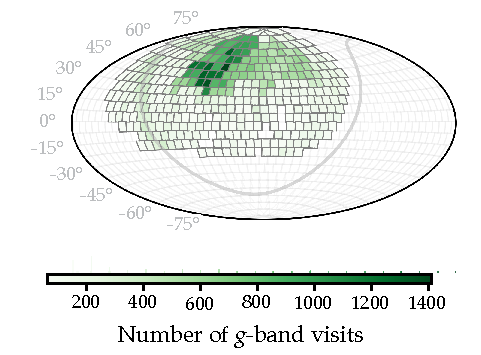
\includegraphics{ztf/ztf_g_band_grid3.pdf}
    \caption[ZTF field visits]{Number of ZTF \textit{g}-band field visits during the first week of May 2020. The primary grid fully tiles the sky accessible at Mount Palomar.}
    \labfig{ztf_g_field_visits}
\end{marginfigure}

To enable robotic control, ZTF operates on a fixed primary on-sky grid of so-called \textit{fields}. Each field corresponds to a fixed sky location with an area of \SI{47}{\square\deg}; the telescope exclusively points to those fields. With such a system, some parts of the sky will always fall into the chip gaps (the parts of the FoV that fall between the 16 CCDs). To mitigate that, there exists a \textit{secondary grid} that is diagonally offset from the primary grid, with \SI{0.29}{\degree} average overlap in right ascension, and \SI{0.26}{\degree} in declination \sidecite{Bellm2019a}. Fig. \ref{fig:ztf_g_field_visits} shows the primary grid and the number of visits per field in the \textit{g}-band during the first week of May 2020.

\section{Calibration and Image Processing}
The ZTF image processing can be divided into two parts: The science exposures are taken at Mount Palomar, while calibration, extraction of transients and archival storage happens at the Infrared Processing and Analysis Center (IPAC)\sidenote{\url{https://www.ipac.caltech.edu}} situated on the campus of the California Institute of Technology (Caltech). IPAC ultimately hosts the ZTF images as part of IRSA\sidenote{\url{https://irsa.ipac.caltech.edu}}, the Infrared Science Archive.

\begin{marginfigure}
    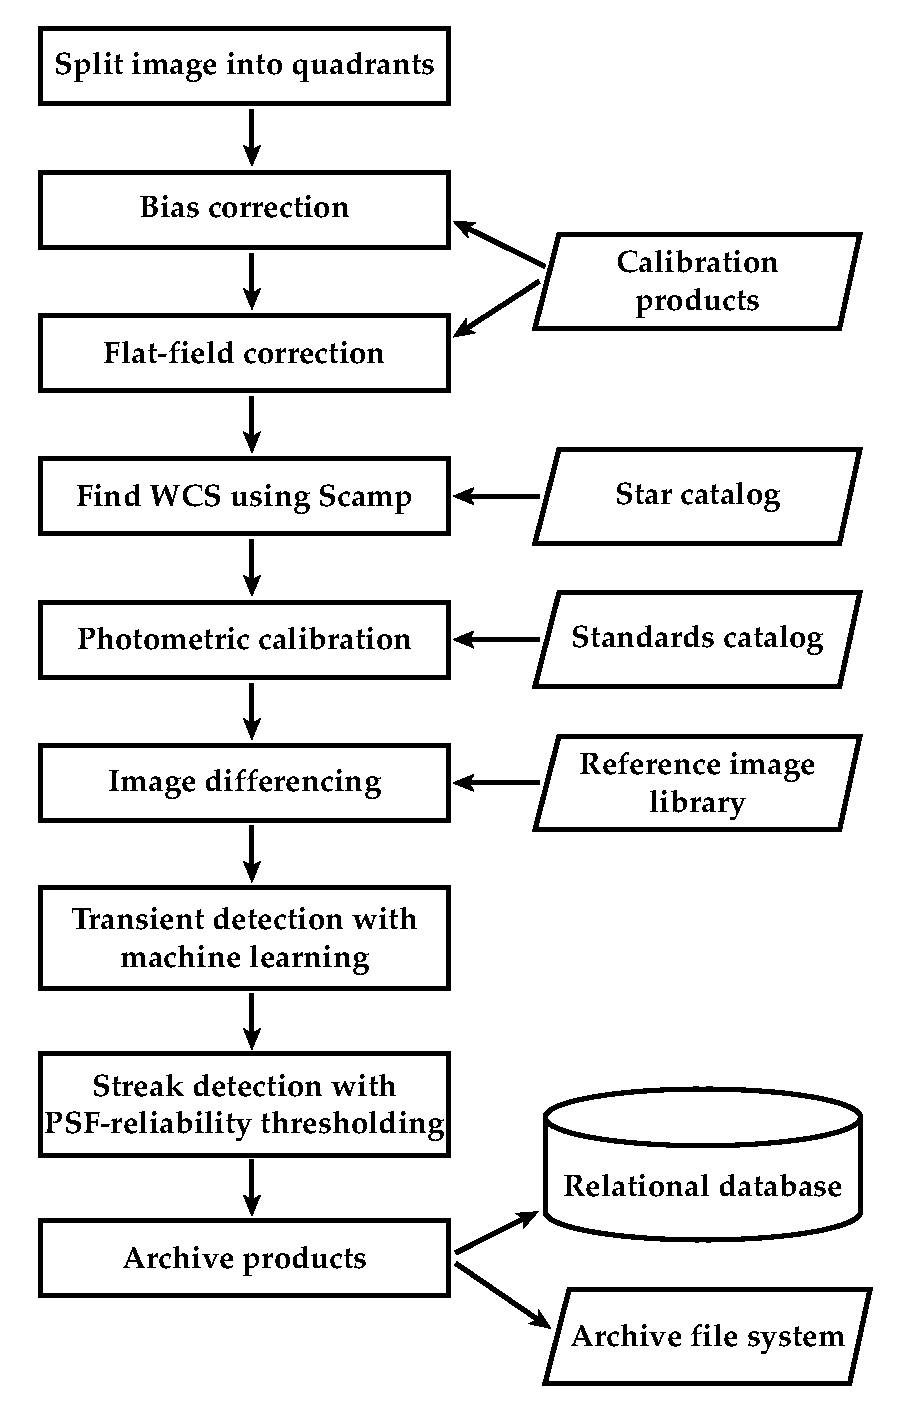
\includegraphics{ztf/ztf_calibration_flow.pdf}
    \caption[ZTF realtime flowchart]{Flowchart of the ZTF calibration, starting with the raw images on the top and ending with the final science products on the bottom. Adapted from \cite{Laher2018}.}
    \labfig{ztf_calibration_flow}
\end{marginfigure}

The full calibration and image processing pipeline is shown in Fig. \ref{fig:ztf_calibration_flow}. First come the different calibration steps: overscan and bias correction, flat fielding, as well as astrometric and photometric calibration. This is followed by creating the difference images and finally extracting the sources. I will briefly explain the different steps in the next sections.

\subsection{On-site processing and datalink}\label{ztf_data_link}

Each image taken on site (calibration and science exposures alike) is stored as FITS file and subsequently compressed loslessly. The compressed images on average use \SI{5}{\bit} per pixel, so the full image is roughly \SI{380}{\mega\byte} large. These images are immediately sent to IPAC with the High Performance Wireless Research \& Educational Network (HPWREN)\sidenote{\url{https://hpwren.ucsd.edu/}}, a microwave-based data network, linking Palomar Observatory with the IPAC post-processing site. Each transfer typically takes \SI{20}{\second}, keeping up with the pace of ZTF observations \cite{Dekany2020}.

\subsection{Overscan correction}
As the temperature of the CCDs changes with time, each image is subject to a time-dependent global offset induced by thermal noise. To correct for this, an \textit{overscan} region is used. In the case of the ZTF CCDs, this region does not correspond to physical pixels, but is created during CCD readout. If one reads out more clock cycles then pixels are available, the charge that has gathered during science readout can be accessed. For ZTF, this is done for an additional 24 cycles, corresponding to 24 overscan pixels for each sensor row. After this, the median of these 24 pixels is taken and the full overscan column is fitted with a quadratic function. For each and every image taken by the camera, the bias described by this quadratic function is calculated and subtracted from the image \cite{Masci2019a}.

\subsection{Bias correction}
The CCD pixels also have different noise levels, meaning in the absence of external photoelectrons they still generate a signal, which is different from pixel to pixel -- i.e. their zero point differs. Luckily, this variation has a higher degree of time-stability \sidecite{Howell2006}. To correct it, at the beginning of each night at least 10 so-called \textit{bias} images are taken and overscan corrected. These images are zero-second exposures which are then stacked. After this, the truncated mean of each pixel is calculated, constituting the final bias image for the night (and filter). This bias image is subtracted from each science exposure using the respective filter taken during the night \cite{Masci2019a}.

\subsection{Flat fielding}
The pixels in the CCDs do not only differ in zero point, they also have slightly different gain or quantum efficiency. This means, their response to light is not uniform. To account for this, the calibration needs a structureless, uniformly bright light source against which the individual pixel response can be measured \cite{Howell2006}. In the case of ZTF, this is achieved by using a flat field illuminator consisting of a round screen illuminated by eight identical boards with LEDs, each board housing $4\times15=60$ LEDs of 15 different colors, covering the full wavelength region of ZTF \cite{Dekany2020}.
\begin{marginfigure}
    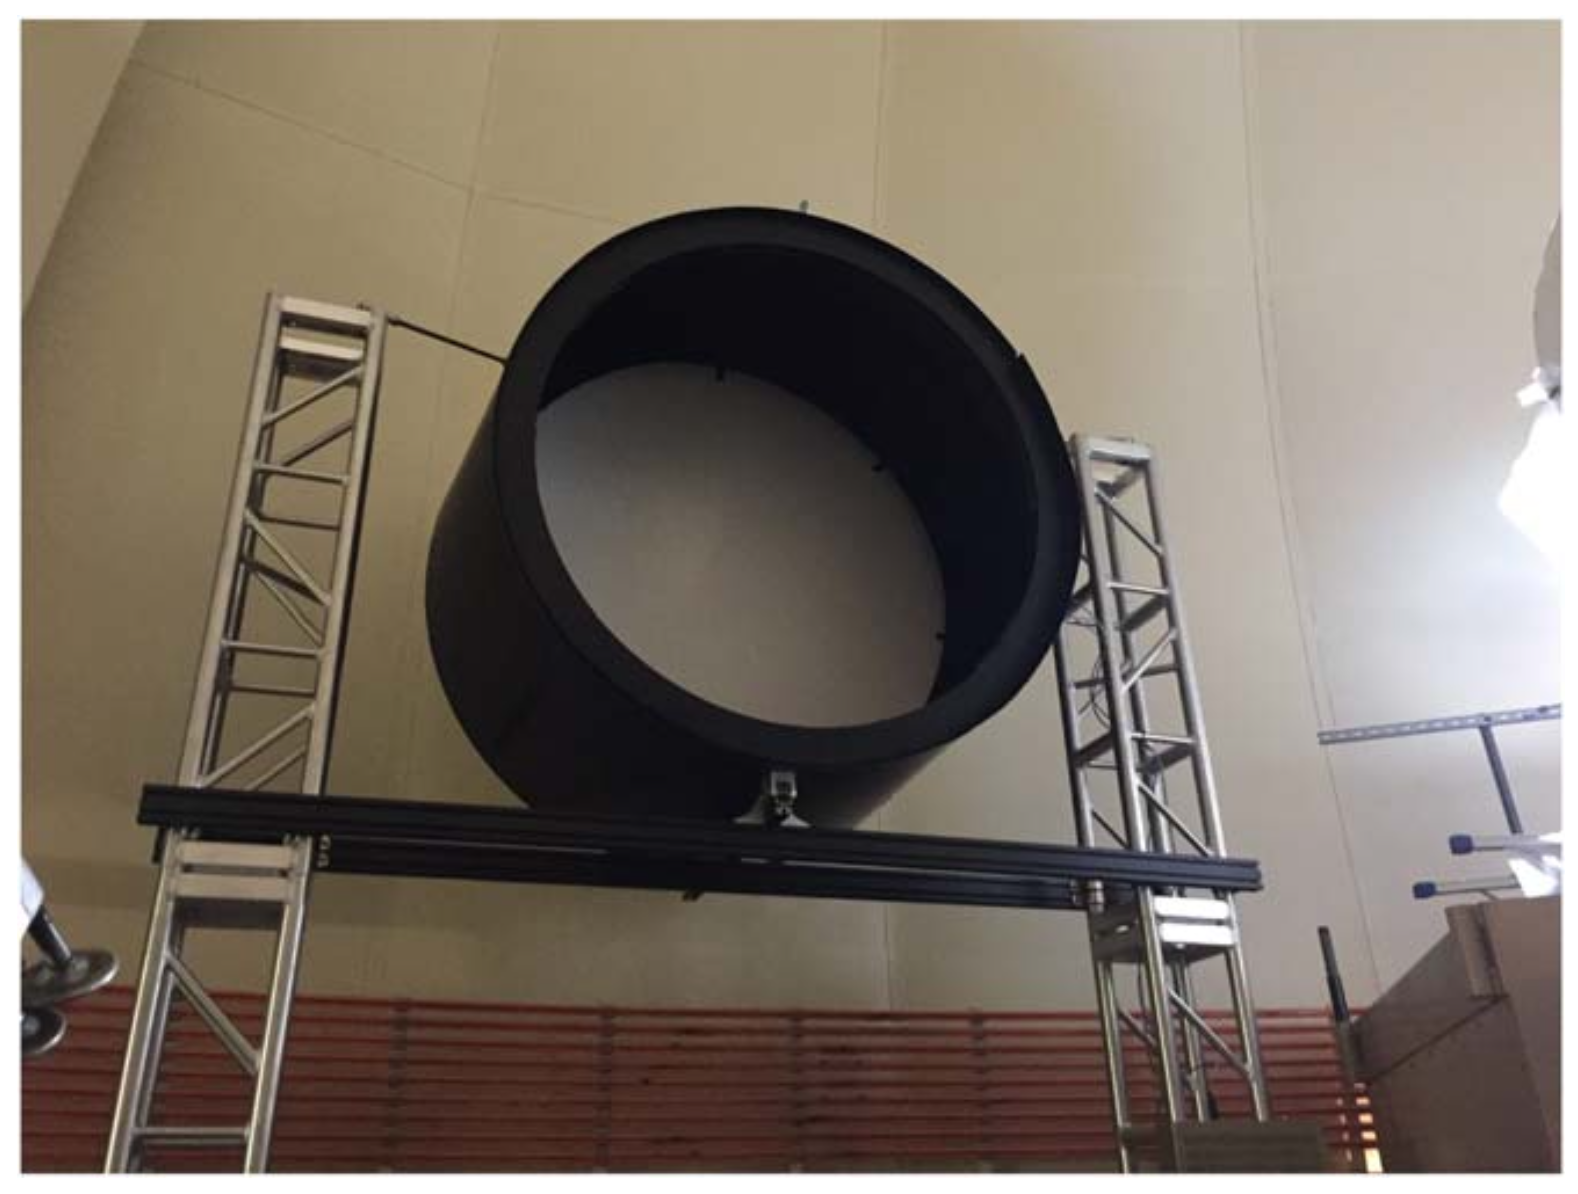
\includegraphics{ztf/ztf_flatfield_illuminator.png}
    \caption[ZTF flat field illuminator]{The ZTF flat field illuminator. From \cite{Dekany2020}.}
    \labfig{ztf_flatfield_illuminator}
\end{marginfigure}
Each afternoon, before science operations begin, at least 20 images per filter are taken of the flat field illuminator. These are then overscan corrected, the bias image is subtracted, and the pixel values are normalized to a truncated global mean of 1 over the image (to allow for later division). After this individual treatment, all flat field images per filter are stacked to a truncated mean per pixel and outlier rejection is applied to isolate additional noisy pixels. All science images taken during the night are divided by this flat field image \cite{Masci2019a}.

\subsection{Astrometric calibration}
Astrometric calibration is the mapping of image pixel coordinates to an on-sky coordinate system. For ZTF, this is performed with stars contained in the \textit{Gaia} Data Release 1 (\textit{Gaia} DR1, \sidecite{Brown2016}). As it is a mission designated to high-precision astrometry, \textit{Gaia} is the ideal reference for this task. Prior to cuts, the DR1 contains over 1 Billion sources. From these, sources are selected that are neither too faint, nor run risk of saturating the detector ($12 \leq G \leq 18$ mag). The astrometric solution is derived using the \texttt{SCAMP} \sidecite{Bertin2006} package \sidecite{Masci2019}. For this, stars are extracted with \texttt{SExtractor} \sidecite{Bertin1996} and matched to the \textit{Gaia} stars. The pointing, rotation and polynomial distortion needed to match the stars constitutes the astrometric solution.

\subsection{PSF photometry} \label{psfphot}
After astrometric calibration, sources in the image need to be extracted to perform photometric calibration (to compare star brightnesses to reference measurements, one first needs stars...). To do so, point spread function (PSF) photometry is employed. Each telescope has a finite aperture, therefore suffering from diffraction. Additionally, earth's atmosphere is constantly and turbulently changing, with different atmospheric layers having different refractive indices, depending on their temperature. This smears out the light from the original point source, an effect known as \textit{seeing} (see Fig. \ref{fig:seeing}).

\begin{figure}[h!]
    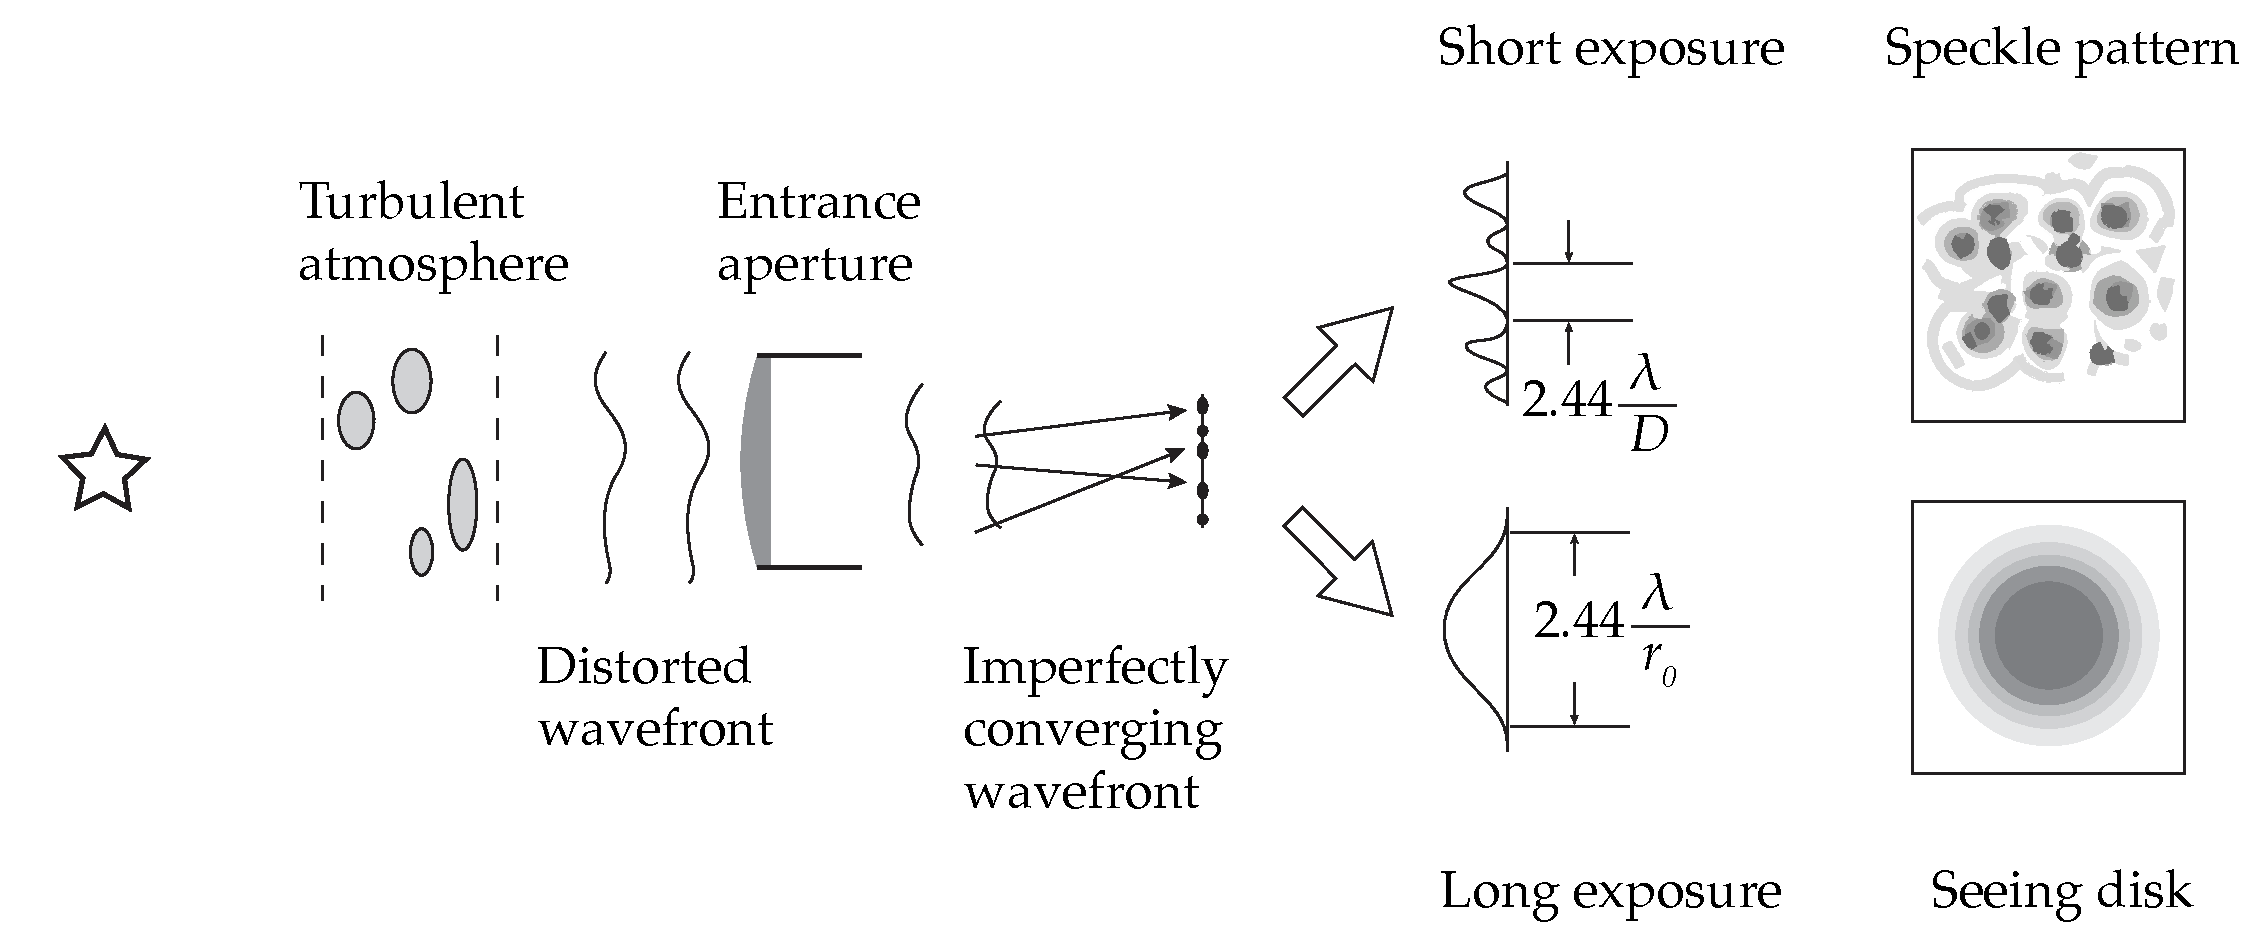
\includegraphics{ztf/seeing.pdf}
    \caption[Seeing]{\textit{Seeing}: Atmospheric distortions cause time-dependent distortions in the wavefronts, which average out during the exposure and form a Gaussian seeing disk on the sensor (bottom right image). Adapted from \cite{Chromey2016}.}
    \labfig{seeing}
\end{figure}

The PSF is describing the way an ideal point source is smeared out spatially after being subjected to atmospheric and optical effects in the telescope, and seeing is the FWHM of the PSF. The algorithm used to reconstruct the PSF of a ZTF exposure is \texttt{DAOphot} \sidecite{Stetson1987}. It fits an analytic Gaussian profile to all point sources within an image. After subtracting this profile, it is iteratively updated with the residuals after subtraction. The background estimate needed for this procedure is extracted from the peak brightness value of a histogram of evenly distributed pixels within the image \cite{Stetson1987}.

\subsection{Photometric calibration and magnitudes} \label{magnitudes}
\marginnote{Of course, PS1 needs to be calibrated in itself. That is done in two steps: A self-consistent relative calibration is created with \texttt{Ubercal} \cite{Schlafly2012}. This relative calibration is in turn anchored to precisely measured \textit{Calspec} standard stars. For details, see \cite{Magnier2020}.}
Not only the source positions in the images need to be calibrated (astrometry), but their brightness as well (photometry). To simplify matters, ZTF is photometrically calibrated against a reference survey, namely PS1. To do this, a catalog of useful calibrator stars from the PS1 survey has been curated. These stars are required to fulfill some basic quality criteria: They should be stable over multiple PS1 survey epochs in all PS1 filters excluding the \textit{y}-band (\textit{g}, \textit{r}, \textit{i}, \textit{z}) and should be fairly bright, but not so bright that they saturate the ZTF sensors. Furthermore, they are required to be fairly isolated to avoid blending with neighboring objects and need to have a high probability of being in fact stars (as opposed to galaxies) \cite{Masci2019a}.

The brightness of both ZTF and PS1 are measured in magnitudes. Magnitudes are somewhat counterintuitive, as a higher value corresponds to a fainter source.\sidenote{This can be traced back over 2000 years to Greek/Roman astronomers Hipparchus and Ptolemy \cite{Krisciunas2001}. These classified the brightest stars to be of ``first order'' or ``first magnitude'', with subsequently dimmer stars assigned lower magnitudes until the dimmest stars visible to the naked eye were of ``sixth magnitude''. The system stuck and was put on firm footing by Norman Pogson in 1856. He defined a star being 5 magnitudes brighter than another one to be 100 times brighter \cite{Jones1968}.} The following definition holds:

\begin{definition}
\labdef{magnitude}
A star one magnitude brighter than another star is $\sqrt[5]{100} \approx 2.512$ times brighter
\end{definition}
If one uses flux density (power per unit area) on earth as a measure of brightness, it follows from Def. \ref{def:magnitude} that the difference between two objects with magnitudes $m_1$ and $m_2$ and respective flux densities $f_1$ and $f_2$ is:
\begin{equation}
m_1 - m_2 = -2.5 \log_{10}{\frac{f_1}{f_2}}
\end{equation}
Now we have a \textit{relative} definition of an source's magnitude, but we need an absolute one. In other words, one needs to know what constitutes a magnitude of 0 (the zero point of the magnitude scale). ZTF uses AB magnitudes \sidecite{Oke1983}, which are defined via the spectral flux density $f_\nu$ [\unit{\W\per\m\per\Hz}]. In this sytem, the magnitude is a logarithm of the spectral flux density: 

\begin{definition}
\labdef{abmag_density}
$m_{\text{AB}}(\nu) = -2.5 \log_{10}{(f_\nu/\SI{3631}{\jansky})}$
\end{definition}

As one can see, a source with constant spectral flux density $f_{\nu,0} = \SI{3631e-23}{\W\per\cm\per\Hz} = \SI{3631}{\jansky}$ corresponds to a magnitude of 0.\sidenote{The value of $f_\nu,0$ is not entirely random: The traditional zero point was the star Vega. Vega's magnitude in the AB system as defined above, integrated over the \textit{V}-band, is 0.03, close to the traditional 0. The AB system has the advantage of not relying on a physical source.} Now, telescopes like ZTF and PS1 use bandpass filters, so the spectral flux density is integrated over the filter wavelengths. Therefore, the magnitude definition changes to \sidecite{Tonry2012}:

\begin{definition}
\labdef{abmag}
$m = -2.5 \log_{10}{\frac{\int{f_\nu(h \nu)^{-1}A(\nu)\,d\nu}}{\int{\SI{3631}{\jansky}(h \nu)^{-1}A(\nu)\,d\nu }}}$
\end{definition}
Here, $h$ is Planck's constant and $A(\nu)$ is the capture cross section (i.e. the chance of an incoming photon to produce an electron in the detector\sidenote{More general, $A(\nu)$ is $A(\nu,\theta,t)$, also depending on the angle of the incoming photon and therefore the atmospheric column along the line of sight, as well as time.}). ZTF does not use a precisely modeled response function $A(\nu)$, but relies on PS1. To first order, ZTF magnitudes are tied to the PS1 system via their zero point:

\begin{equation}
m_\text{cal} = m_\text{instr} + \text{ZP}
\end{equation}

To do this, all extracted sources are spatially matched to the PS1 calibrator catalog. After creating a one-to-one relation between ZTF stars and PS calibrator stars, one could to first order calculate $m_\text{cal}$.

But there is a potential complication: The ZTF and PS1 filters are fairly similar, but not exactly so. This means that a celestial object that does not have a constant spectrum (i.e. almost all of them) will have slightly different brightness values when measured with the ZTF and the corresponding PS1 filter. To account for this, a linear, filter-dependent \textit{color correction} $c_f$ needs to be applied:

\begin{equation}
m_\text{cal} = m_\text{instr} + \text{ZP}_f + c_f \times \text{PS1}_\text{clr}
\end{equation}
where $\text{PS1}_\text{clr}$ is filter dependent ($g_\text{PS1}-r_\text{PS1}$ for the ZTF \textit{g}/\textit{r}-band, and $r_\text{PS1}-i_\text{PS1}$ for the \textit{i}-band).

In the photometric calibration step, $\text{ZP}_f$ and $c_f$ are chosen to globally minimize $\Delta m_f = \text{ZP}_f + c_f \times \text{PS1}_\text{clr}$ for all calibrator stars in the respective image \cite{Masci2019a}.

\subsection{Image subtraction} \label{ztf_image_subtraction}
Because ZTF is a survey telescope deeply rooted in time-domain astronomy, many of the science goals concern observing sources that are \textit{new} or \textit{changing}. To do so, one needs to detect changes in the nightly observations with regard to \textit{reference images}. From all new images those reference images are subtracted (see Fig. \ref{fig:img_subtraction}). All remaining detections constitute temporal evolution with respect to the epoch of reference image creation. All reference images in ZTF are stacked images of 15--40 individual high-quality images, most of them created early after the start of telescope operations. Quality criteria for the individual images comprise good seeing, low errors on the astrometric and photometric calibrations, as well as background levels falling into filter-specific ranges \cite{Masci2019}.

\texttt{SWarp} \sidecite{Bertin2010} is used to interpolate and resample the reference image onto the science image, while subsequent subtraction and PSF photometry (see Section \ref{psfphot}) is performed with the \texttt{ZOGY} algorithm \sidecite{Zackay2016}.

\begin{figure}[h!]
    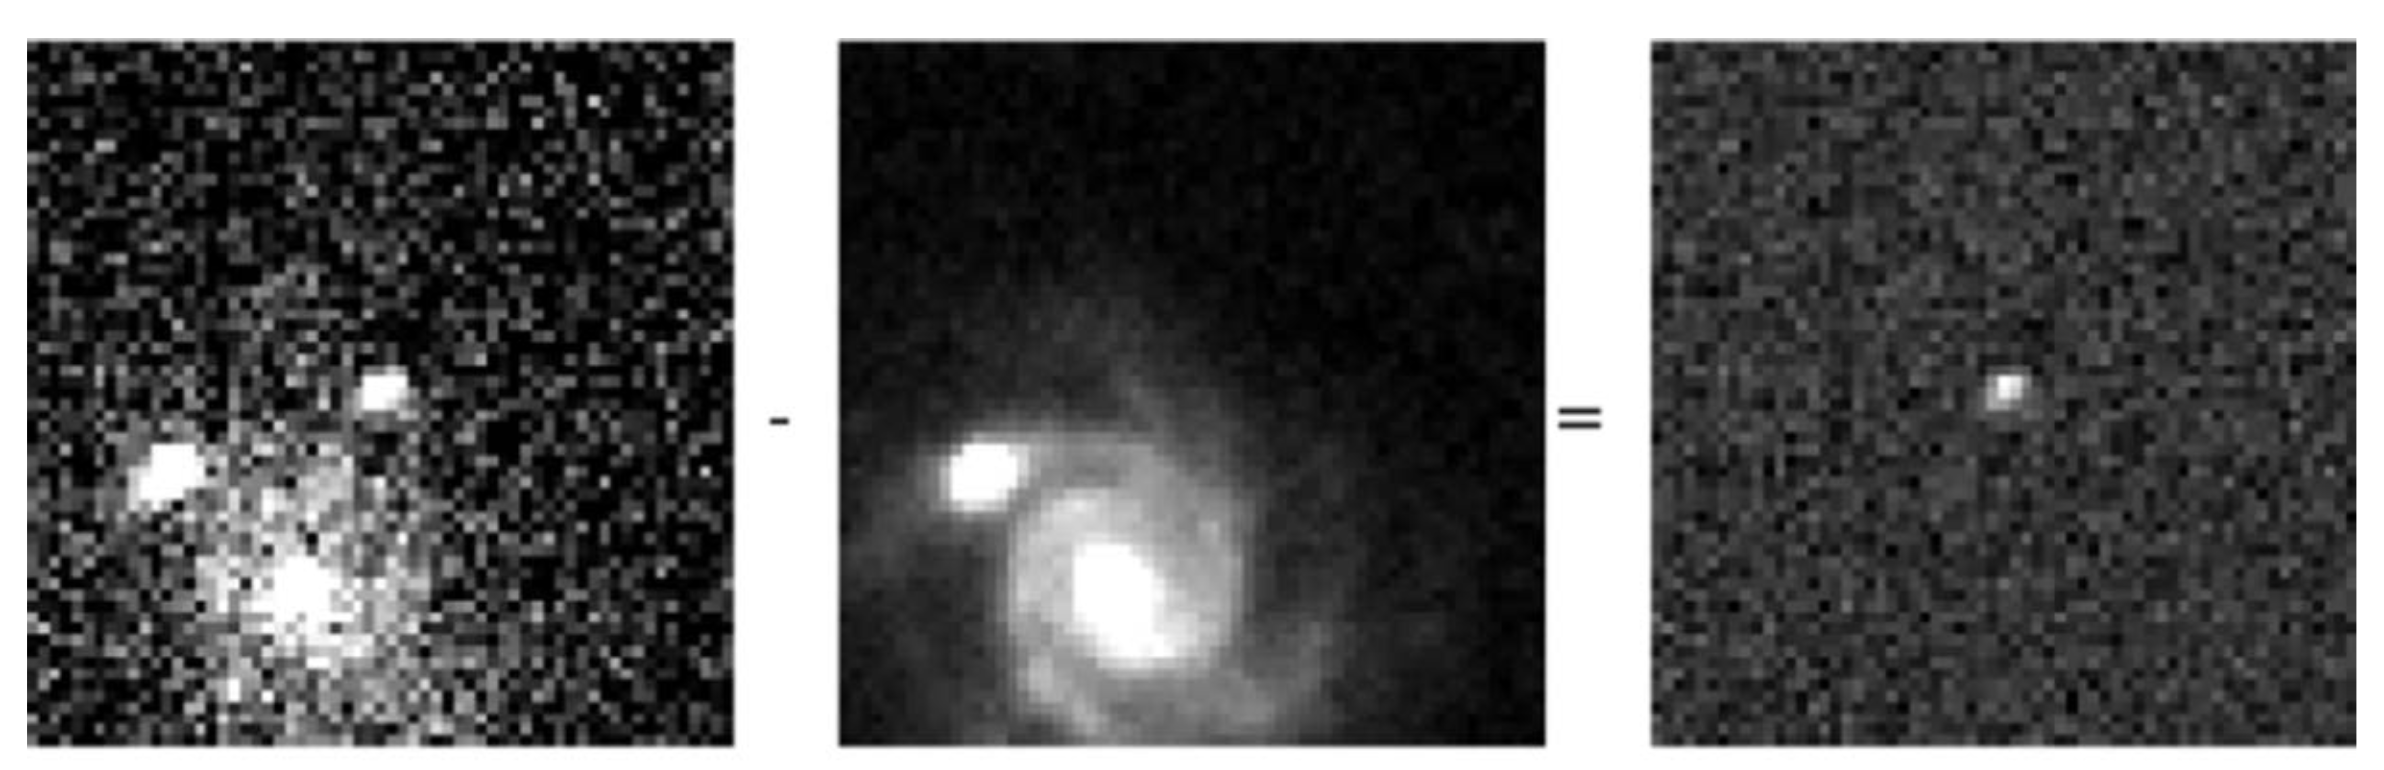
\includegraphics{ztf/ztf_imsub.png}
    \caption[ZTF image subtraction]{ZTF image subtraction. The new science image is on the left; in the middle is reference image, which is subtracted. This results in a \textit{difference image}, seen on the right. From \cite{Mahabal2019}.}
    \labfig{img_subtraction}
\end{figure}

\subsection{Alert packages} \label{ztf_alerts}
\begin{marginfigure}
    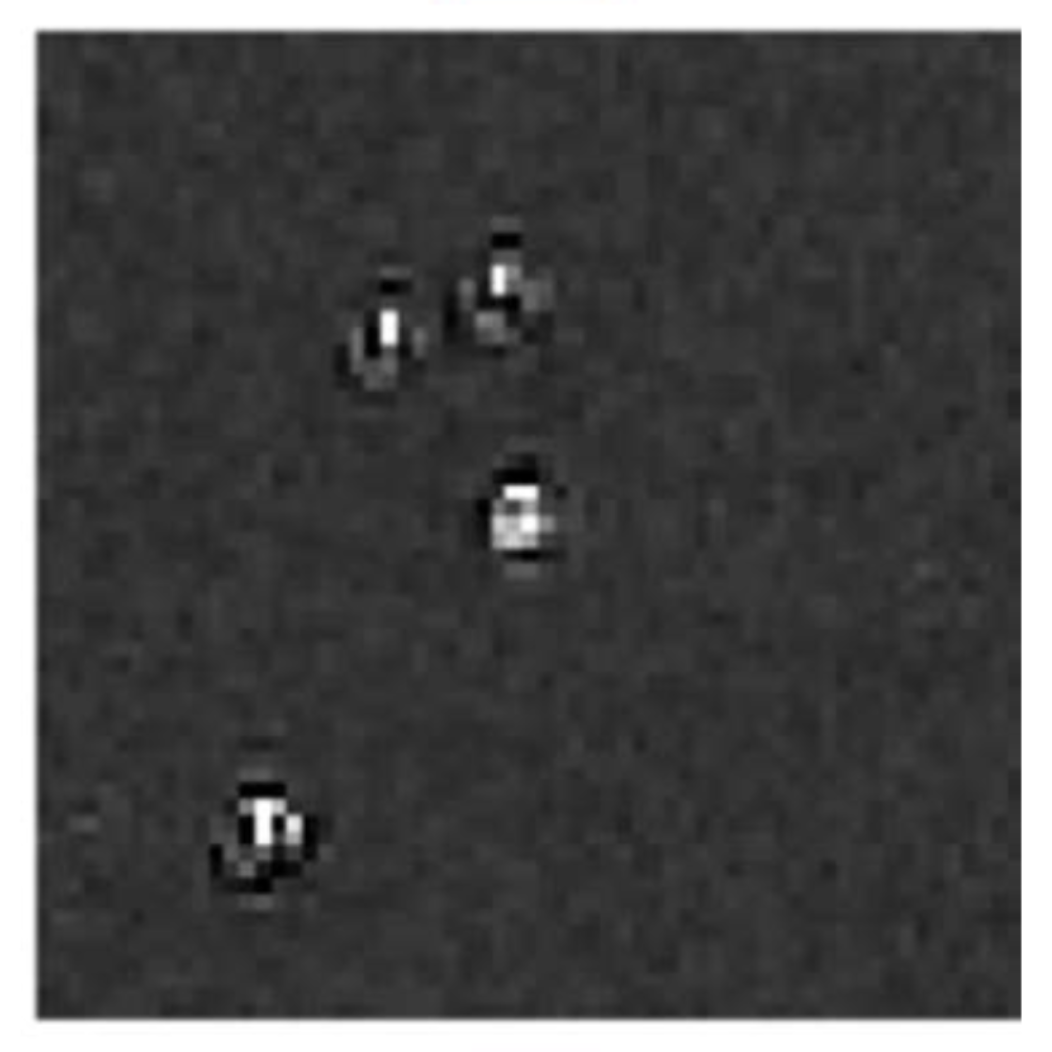
\includegraphics{ztf/ztf_bogus.png}
    \caption[ZTF subtraction artifact]{ZTF subtraction artifact, resulting in a bogus transient. From \cite{Mahabal2019}.}
    \labfig{ztf_bogus}
\end{marginfigure}

The last step in the imaging pipeline is alerting an array of upstream transient alert brokers. The information on new transients or updates on existing ones therefore need to be packaged into a convenient format. All positive detections after image subtraction with a signal-to-noise greater than 5 are subjected to \texttt{RealBogus}. This is a machine learning (ML) algorithm trained to discriminate between ``real'' events (most likely astrophysical) and ``bogus'' events (e.g. subtraction artifacts, see Fig. \ref{fig:ztf_bogus}) \sidecite{Mahabal2019}. This algorithm creates a \texttt{rbscore}, ranking the probability of the detection of being real.

Another ML algorithm has been employed to assign all PS1 sources a \texttt{sgscore}, separating between stars and galaxies based on their morphology and flux in all PS1 bands \sidecite{Tachibana2018}. Both \texttt{rbscore} and \texttt{sgscore}, as well as cutouts of the science, reference and difference images are packed together and shipped as \textit{alert package}. These alerts also include the distances to the three nearest PS1 sources, the closest \textit{Gaia} source, up to 30 days of previous detections if these exist, and some quality metrics like the limiting magnitude. The file format for distribution is Apache Avro\sidenote{\url{https://avro.apache.org}}, and the method of distribution is an Apache Kafka\sidenote{\url{https://kafka.apache.org}} stream \sidecite{Patterson2018}.

\section{Surveys and Cadence}
ZTF is supporting three main survey programs: First, there is the NSF Mid-Scale Innovations Program (MSIP) survey, which is allocated \SI{40}{\percent} of telescope time. The MSIP survey is subdivided into the Northern Sky Survey, using a large fraction (\SI{85}{\percent}) of MSIP time. This survey covers the entire \SI{23675}{\square\deg} of the northern sky \SI{7}{\degree} above the galactic plane. As long as a field (see Section \ref{ztf_grid}) is accessible, it is observed once in the \textit{g}- and once in the \textit{r}-band every 3 nights, with both images separated by at least 30 minutes to reject transients and moving (i.e. solar system) objects. The rest of the northern sky ($|b|\leq \SI{7}{\degree}$, with a footprint of \SI{2800}{\square\deg}) is visited twice per night, with the same observational parameters as the Northern Sky Survey \cite{Bellm2019a}.

Another \SI{40}{\percent} are allocated to the partners of the ZTF collaboration. During the first year of ZTF operation, this allocation was dedicated to the Extragalactic High Cadence Survey, the \textit{i}-band Survey, to ToO observations like the Neutrino Follow-up Program (see Chapter \ref{fupipeline}), to the Twilight Survey, the High-cadence Plane Survey and the Asteroid Rotation Period Survey \cite{Bellm2019a}.

The last \SI{20}{\percent} are private Caltech time, with surveys selected each semester by the Caltech Time Allocation Committee \cite{Bellm2019a}. A prominent example is the observational campaign to follow up 
LIGO-Virgo (LV) \sidecite{Aasi2015,Acernese2014} gravitational wave (GW) localizations during the 3rd observational run (O3) \sidecite{Kasliwal2020}.

\setchapterimage[7cm]{fu/heading3.png}
\chapter{The ZTF Follow-Up Pipeline} 
\labch{fupipeline}
After introducing the IceCube detector (see chapter \ref{ic}) and the Zwicky Transient Facility (see chapter \ref{ztf}), we now have all the ingredients to introduce the ZTF high-energy neutrino follow-up pipeline.

IceCube sends out \num{\sim2.2} astrophysical high-energy neutrino alerts on average per month (see section \ref{ic_alerts}). Due to its large FoV and fully robotic operation, ZTF is the ideal follow-up instrument for these alerts. The typically reported IceCube localization regions can be covered with only one pointing of the telescope.

The follow-up procedure can be outlined as follows: An \textit{IceCube alert} is received. If the alert meets our \textit{alert quality criteria}, we do an \textit{observability check}. If the sky region is accessible to ZTF, we \textit{observe}. After observations, we \textit{filter} candidates with \texttt{AMPEL} \sidecite{Nordin2019}, followed by visual inspection and -- if needed -- trigger \textit{additional follow-up}.

\section{Alert cuts}\label{alert_cuts}
As we only have limited telescope time, we apply quality cuts on the high-energy neutrino alerts received via GCN. As outlined in section \ref{ic_event_selection}, there are two alert streams: \textit{Gold alerts} with an average purity of \SI{50}{\percent} (\SI{36}{\percent} of all non-retracted alerts), and \textit{bronze alerts} with an average purity of \SI{30}{\percent} (\SI{64}{\percent}).

In general, we only follow up if the reported rectangular \SI{90}{\percent} uncertainty region is smaller than \SI{40}{\square\deg}. All gold alerts making this cut qualify for follow up. There is a more stringent cut on the uncertainty area of bronze alerts, requiring these are $<\SI{10}{\square\deg}$.

\section{Observation planning with \texttt{planobs}}\label{planobs}
If an alert makes the cut, one needs to check if observations with ZTF are feasible. To reduce the potential for errors, this is done with assistance by the \texttt{planobs} \sidecite{Reusch2023} tool, developed mainly by the author to automate the task as much as possible.

\texttt{planobs} is written in Python, and is deployed on a virtual private server. The backend runs on \texttt{Flask}\sidenote{\url{https://flask.palletsprojects.com}} behind a \texttt{nginx}\sidenote{\url{https://www.nginx.com}} reverse proxy and serves a Slack\sidenote{\url{https://slack.com/}} bot integrated into the DESY multimessenger group chat.

The tool is constructed to be used with a simple command-line-style interface in the Slack chat. For example, 
\begin{lstlisting}[language=bash,style=kaolstplain]
Plan IC221223A -multiday
\end{lstlisting}
will create an observation plan for IceCube high-energy neutrino IC220501A, spanning multiple days.

To obtain the positional and error information on the neutrino in question from the respective GCN circular, \texttt{planobs} is searching for the GCN on an experimental server\sidenote{\url{https://heasarc.gsfc.nasa.gov/wsgi-scripts/tach/gcn_v2/tach.wsgi}}. As notices are written by humans, it fuzzily parses them to extract the relevant information. After this, observability at Mt. Palomar is calculated, defaulting to the current time (optionally, a desired observation time can be requested). 

\begin{figure}[h!]
    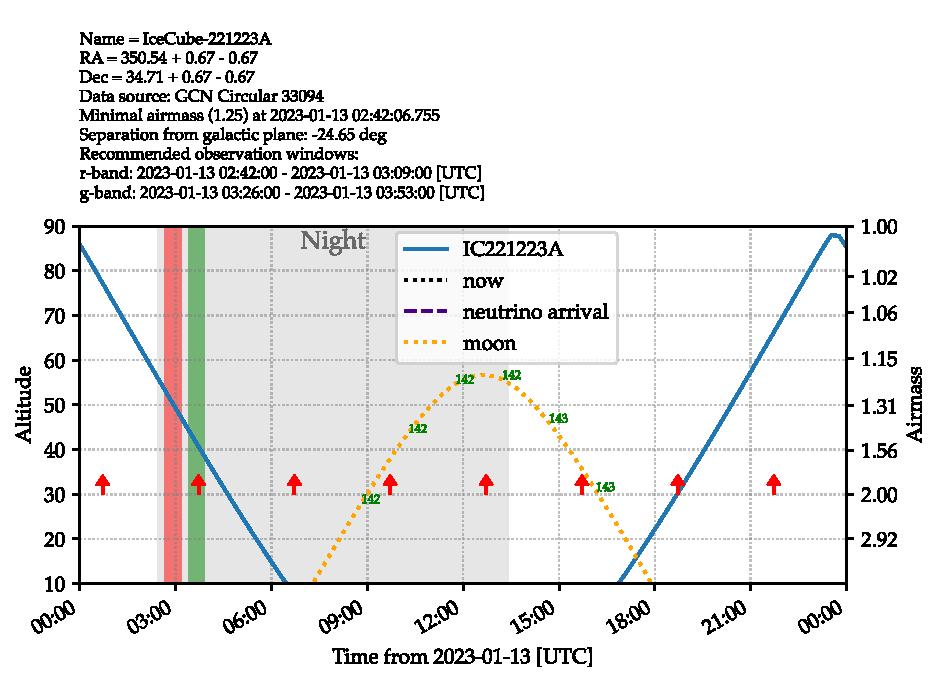
\includegraphics{fu/planobs_airmass.pdf}
    \caption[Observation plan]{Observation plot created by \texttt{planobs} for the follow-up of IceCube neutrino IC221223A. The altitude and airmass of the alert region at Mt. Palomar are shown in blue. The red and green shaded regions are proposed observation windows in the \textit{r}- and \textit{r}-band. The red arrows show the airmass limit of 2.0, and the moon is displayed as yellow dotted curve. The gray shaded region marks night-time at the telescope site. All information automatically extracted from the GCN circular are shown on top.}
    \labfig{planobs}
\end{figure}
\begin{marginfigure}
    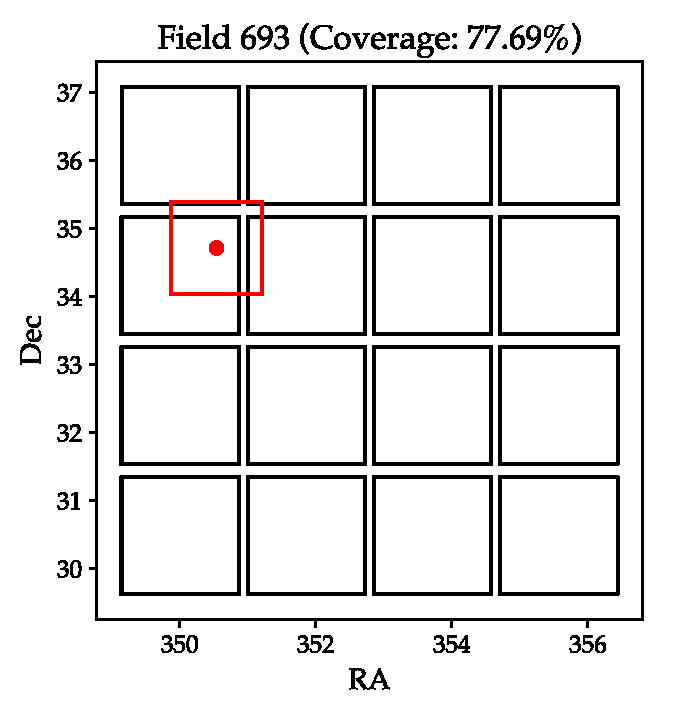
\includegraphics{fu/planobs_grid.pdf}
    \caption[\texttt{planobs} ZTF grid]{The ZTF grid overlaid on the \SI{90}{\percent} uncertainty rectangle.}
    \labfig{planobs_grid}
\end{marginfigure}
An example observability plot is shown in Fig. \ref{fig:planobs}. The blue curve shows the altitude of the sky region in question above Mt. Palomar, and the red and green shaded regions mark the two proposed observation windows in the \textit{r}- and the \textit{g}-band.

Additionally, for each field within the primary and secondary grid (see section \ref{ztf_grid}) that have overlap with the uncertainty region\sidenote{There is an additional check to ensure the fields have reference images available, see section \ref{ztf_image_subtraction}.}, the coverage is calculated and the field with the highest coverage is selected. Fig. \ref{fig:planobs_grid} shows such an overlay plot for IC221223A and ZTF field 693.

If the plan looks good, one needs to invoke
\begin{lstlisting}[language=bash,style=kaolstplain]
Plan IC221223A -trigger
\end{lstlisting} 
to submit the observation request via a dedicated API to the telescope scheduler. There is additional functionality to ensure that the trigger has been added to the telescope queue. If all goes well and weather permits, the observations are carried out, and candidate vetting can begin.

As we are interested in the evolution of potential source candidates, usually observations within a \SI{10}{\day} window are triggered. To obtain deep images during the first night, we trigger \SI{300}{\second} exposures in the \textit{g}- and \textit{r}-band in the first night. These are followed by shallower \SI{30}{\second} observations in the \textit{g}-band during nights 2, 3, 5 and 7, and finally shallow observations in both \textit{g}- and \textit{r}-band during night 9.

\section{The \texttt{AMPEL} broker}
The next step in the pipeline is the selection of good candidates. ZTF typically serves $\mathcal{O}(\numrange{e5}{e6})$ alerts per night\todo{JvS!}. As only a fraction of those is relevant for us, we need software to cut down the number of alerts. This is exactly what AMPEL is doing, a streaming data analysis framework developed at Humboldt-University Berlin and DESY Zeuthen.




%\chapter{Candidate TDE AT2019fdr: a possible source?}
%\chapter{The ZTF nuclear sample}
%\chapter{Conclusion and Outlook}
\appendix

\pagelayout{wide} % No margins
\addpart{Appendix}
\pagelayout{margin} % Restore margins


%----------------------------------------------------------------------------------------

\backmatter % Denotes the end of the main document content
\setchapterstyle{plain} % Output plain chapters from this point onwards 

%----------------------------------------------------------------------------------------
%   BIBLIOGRAPHY
%----------------------------------------------------------------------------------------

% The bibliography needs to be compiled with biber using your LaTeX editor, or on the command line with 'biber main' from the template directory
%\defbibnote{bibnote}{Here are the references in citation order.\par\bigskip} % Prepend this text to the bibliography
\printbibliography[heading=bibintoc, title=Bibliography] % Add the bibliography heading to the ToC, set the title of the bibliography and output the bibliography note

%----------------------------------------------------------------------------------------
%   INDEX
%----------------------------------------------------------------------------------------

% The index needs to be compiled on the command line with 'makeindex main' from the template directory

\printindex % Output the index

\end{document}
